


% Header, overrides base

    % Make sure that the sphinx doc style knows who it inherits from.
    \def\sphinxdocclass{article}

    % Declare the document class
    \documentclass[letterpaper,10pt,english]{/anaconda/lib/python2.7/site-packages/sphinx/texinputs/sphinxhowto}

    % Imports
    \usepackage[utf8]{inputenc}
    \DeclareUnicodeCharacter{00A0}{\\nobreakspace}
    \usepackage[T1]{fontenc}
    \usepackage{babel}
    \usepackage{times}
    \usepackage{import}
    \usepackage[Bjarne]{/anaconda/lib/python2.7/site-packages/sphinx/texinputs/fncychap}
    \usepackage{longtable}
    \usepackage{/anaconda/lib/python2.7/site-packages/sphinx/texinputs/sphinx}
    \usepackage{multirow}

    \usepackage{amsmath}
    \usepackage{amssymb}
    \usepackage{ucs}
    \usepackage{enumerate}

    % Used to make the Input/Output rules follow around the contents.
    \usepackage{needspace}

    % Pygments requirements
    \usepackage{fancyvrb}
    \usepackage{color}
    % ansi colors additions
    \definecolor{darkgreen}{rgb}{.12,.54,.11}
    \definecolor{lightgray}{gray}{.95}
    \definecolor{brown}{rgb}{0.54,0.27,0.07}
    \definecolor{purple}{rgb}{0.5,0.0,0.5}
    \definecolor{darkgray}{gray}{0.25}
    \definecolor{lightred}{rgb}{1.0,0.39,0.28}
    \definecolor{lightgreen}{rgb}{0.48,0.99,0.0}
    \definecolor{lightblue}{rgb}{0.53,0.81,0.92}
    \definecolor{lightpurple}{rgb}{0.87,0.63,0.87}
    \definecolor{lightcyan}{rgb}{0.5,1.0,0.83}

    % Needed to box output/input
    \usepackage{tikz}
        \usetikzlibrary{calc,arrows,shadows}
    \usepackage[framemethod=tikz]{mdframed}

    \usepackage{alltt}

    % Used to load and display graphics
    \usepackage{graphicx}
    \graphicspath{ {figs/} }
    \usepackage[Export]{adjustbox} % To resize

    % used so that images for notebooks which have spaces in the name can still be included
    \usepackage{grffile}


    % For formatting output while also word wrapping.
    \usepackage{listings}
    \lstset{breaklines=true}
    \lstset{basicstyle=\small\ttfamily}
    \def\smaller{\fontsize{9.5pt}{9.5pt}\selectfont}

    %Pygments definitions
    
\makeatletter
\def\PY@reset{\let\PY@it=\relax \let\PY@bf=\relax%
    \let\PY@ul=\relax \let\PY@tc=\relax%
    \let\PY@bc=\relax \let\PY@ff=\relax}
\def\PY@tok#1{\csname PY@tok@#1\endcsname}
\def\PY@toks#1+{\ifx\relax#1\empty\else%
    \PY@tok{#1}\expandafter\PY@toks\fi}
\def\PY@do#1{\PY@bc{\PY@tc{\PY@ul{%
    \PY@it{\PY@bf{\PY@ff{#1}}}}}}}
\def\PY#1#2{\PY@reset\PY@toks#1+\relax+\PY@do{#2}}

\expandafter\def\csname PY@tok@gd\endcsname{\def\PY@tc##1{\textcolor[rgb]{0.63,0.00,0.00}{##1}}}
\expandafter\def\csname PY@tok@gu\endcsname{\let\PY@bf=\textbf\def\PY@tc##1{\textcolor[rgb]{0.50,0.00,0.50}{##1}}}
\expandafter\def\csname PY@tok@gt\endcsname{\def\PY@tc##1{\textcolor[rgb]{0.00,0.27,0.87}{##1}}}
\expandafter\def\csname PY@tok@gs\endcsname{\let\PY@bf=\textbf}
\expandafter\def\csname PY@tok@gr\endcsname{\def\PY@tc##1{\textcolor[rgb]{1.00,0.00,0.00}{##1}}}
\expandafter\def\csname PY@tok@cm\endcsname{\let\PY@it=\textit\def\PY@tc##1{\textcolor[rgb]{0.25,0.50,0.50}{##1}}}
\expandafter\def\csname PY@tok@vg\endcsname{\def\PY@tc##1{\textcolor[rgb]{0.10,0.09,0.49}{##1}}}
\expandafter\def\csname PY@tok@m\endcsname{\def\PY@tc##1{\textcolor[rgb]{0.40,0.40,0.40}{##1}}}
\expandafter\def\csname PY@tok@mh\endcsname{\def\PY@tc##1{\textcolor[rgb]{0.40,0.40,0.40}{##1}}}
\expandafter\def\csname PY@tok@go\endcsname{\def\PY@tc##1{\textcolor[rgb]{0.53,0.53,0.53}{##1}}}
\expandafter\def\csname PY@tok@ge\endcsname{\let\PY@it=\textit}
\expandafter\def\csname PY@tok@vc\endcsname{\def\PY@tc##1{\textcolor[rgb]{0.10,0.09,0.49}{##1}}}
\expandafter\def\csname PY@tok@il\endcsname{\def\PY@tc##1{\textcolor[rgb]{0.40,0.40,0.40}{##1}}}
\expandafter\def\csname PY@tok@cs\endcsname{\let\PY@it=\textit\def\PY@tc##1{\textcolor[rgb]{0.25,0.50,0.50}{##1}}}
\expandafter\def\csname PY@tok@cp\endcsname{\def\PY@tc##1{\textcolor[rgb]{0.74,0.48,0.00}{##1}}}
\expandafter\def\csname PY@tok@gi\endcsname{\def\PY@tc##1{\textcolor[rgb]{0.00,0.63,0.00}{##1}}}
\expandafter\def\csname PY@tok@gh\endcsname{\let\PY@bf=\textbf\def\PY@tc##1{\textcolor[rgb]{0.00,0.00,0.50}{##1}}}
\expandafter\def\csname PY@tok@ni\endcsname{\let\PY@bf=\textbf\def\PY@tc##1{\textcolor[rgb]{0.60,0.60,0.60}{##1}}}
\expandafter\def\csname PY@tok@nl\endcsname{\def\PY@tc##1{\textcolor[rgb]{0.63,0.63,0.00}{##1}}}
\expandafter\def\csname PY@tok@nn\endcsname{\let\PY@bf=\textbf\def\PY@tc##1{\textcolor[rgb]{0.00,0.00,1.00}{##1}}}
\expandafter\def\csname PY@tok@no\endcsname{\def\PY@tc##1{\textcolor[rgb]{0.53,0.00,0.00}{##1}}}
\expandafter\def\csname PY@tok@na\endcsname{\def\PY@tc##1{\textcolor[rgb]{0.49,0.56,0.16}{##1}}}
\expandafter\def\csname PY@tok@nb\endcsname{\def\PY@tc##1{\textcolor[rgb]{0.00,0.50,0.00}{##1}}}
\expandafter\def\csname PY@tok@nc\endcsname{\let\PY@bf=\textbf\def\PY@tc##1{\textcolor[rgb]{0.00,0.00,1.00}{##1}}}
\expandafter\def\csname PY@tok@nd\endcsname{\def\PY@tc##1{\textcolor[rgb]{0.67,0.13,1.00}{##1}}}
\expandafter\def\csname PY@tok@ne\endcsname{\let\PY@bf=\textbf\def\PY@tc##1{\textcolor[rgb]{0.82,0.25,0.23}{##1}}}
\expandafter\def\csname PY@tok@nf\endcsname{\def\PY@tc##1{\textcolor[rgb]{0.00,0.00,1.00}{##1}}}
\expandafter\def\csname PY@tok@si\endcsname{\let\PY@bf=\textbf\def\PY@tc##1{\textcolor[rgb]{0.73,0.40,0.53}{##1}}}
\expandafter\def\csname PY@tok@s2\endcsname{\def\PY@tc##1{\textcolor[rgb]{0.73,0.13,0.13}{##1}}}
\expandafter\def\csname PY@tok@vi\endcsname{\def\PY@tc##1{\textcolor[rgb]{0.10,0.09,0.49}{##1}}}
\expandafter\def\csname PY@tok@nt\endcsname{\let\PY@bf=\textbf\def\PY@tc##1{\textcolor[rgb]{0.00,0.50,0.00}{##1}}}
\expandafter\def\csname PY@tok@nv\endcsname{\def\PY@tc##1{\textcolor[rgb]{0.10,0.09,0.49}{##1}}}
\expandafter\def\csname PY@tok@s1\endcsname{\def\PY@tc##1{\textcolor[rgb]{0.73,0.13,0.13}{##1}}}
\expandafter\def\csname PY@tok@sh\endcsname{\def\PY@tc##1{\textcolor[rgb]{0.73,0.13,0.13}{##1}}}
\expandafter\def\csname PY@tok@sc\endcsname{\def\PY@tc##1{\textcolor[rgb]{0.73,0.13,0.13}{##1}}}
\expandafter\def\csname PY@tok@sx\endcsname{\def\PY@tc##1{\textcolor[rgb]{0.00,0.50,0.00}{##1}}}
\expandafter\def\csname PY@tok@bp\endcsname{\def\PY@tc##1{\textcolor[rgb]{0.00,0.50,0.00}{##1}}}
\expandafter\def\csname PY@tok@c1\endcsname{\let\PY@it=\textit\def\PY@tc##1{\textcolor[rgb]{0.25,0.50,0.50}{##1}}}
\expandafter\def\csname PY@tok@kc\endcsname{\let\PY@bf=\textbf\def\PY@tc##1{\textcolor[rgb]{0.00,0.50,0.00}{##1}}}
\expandafter\def\csname PY@tok@c\endcsname{\let\PY@it=\textit\def\PY@tc##1{\textcolor[rgb]{0.25,0.50,0.50}{##1}}}
\expandafter\def\csname PY@tok@mf\endcsname{\def\PY@tc##1{\textcolor[rgb]{0.40,0.40,0.40}{##1}}}
\expandafter\def\csname PY@tok@err\endcsname{\def\PY@bc##1{\setlength{\fboxsep}{0pt}\fcolorbox[rgb]{1.00,0.00,0.00}{1,1,1}{\strut ##1}}}
\expandafter\def\csname PY@tok@kd\endcsname{\let\PY@bf=\textbf\def\PY@tc##1{\textcolor[rgb]{0.00,0.50,0.00}{##1}}}
\expandafter\def\csname PY@tok@ss\endcsname{\def\PY@tc##1{\textcolor[rgb]{0.10,0.09,0.49}{##1}}}
\expandafter\def\csname PY@tok@sr\endcsname{\def\PY@tc##1{\textcolor[rgb]{0.73,0.40,0.53}{##1}}}
\expandafter\def\csname PY@tok@mo\endcsname{\def\PY@tc##1{\textcolor[rgb]{0.40,0.40,0.40}{##1}}}
\expandafter\def\csname PY@tok@kn\endcsname{\let\PY@bf=\textbf\def\PY@tc##1{\textcolor[rgb]{0.00,0.50,0.00}{##1}}}
\expandafter\def\csname PY@tok@mi\endcsname{\def\PY@tc##1{\textcolor[rgb]{0.40,0.40,0.40}{##1}}}
\expandafter\def\csname PY@tok@gp\endcsname{\let\PY@bf=\textbf\def\PY@tc##1{\textcolor[rgb]{0.00,0.00,0.50}{##1}}}
\expandafter\def\csname PY@tok@o\endcsname{\def\PY@tc##1{\textcolor[rgb]{0.40,0.40,0.40}{##1}}}
\expandafter\def\csname PY@tok@kr\endcsname{\let\PY@bf=\textbf\def\PY@tc##1{\textcolor[rgb]{0.00,0.50,0.00}{##1}}}
\expandafter\def\csname PY@tok@s\endcsname{\def\PY@tc##1{\textcolor[rgb]{0.73,0.13,0.13}{##1}}}
\expandafter\def\csname PY@tok@kp\endcsname{\def\PY@tc##1{\textcolor[rgb]{0.00,0.50,0.00}{##1}}}
\expandafter\def\csname PY@tok@w\endcsname{\def\PY@tc##1{\textcolor[rgb]{0.73,0.73,0.73}{##1}}}
\expandafter\def\csname PY@tok@kt\endcsname{\def\PY@tc##1{\textcolor[rgb]{0.69,0.00,0.25}{##1}}}
\expandafter\def\csname PY@tok@ow\endcsname{\let\PY@bf=\textbf\def\PY@tc##1{\textcolor[rgb]{0.67,0.13,1.00}{##1}}}
\expandafter\def\csname PY@tok@sb\endcsname{\def\PY@tc##1{\textcolor[rgb]{0.73,0.13,0.13}{##1}}}
\expandafter\def\csname PY@tok@k\endcsname{\let\PY@bf=\textbf\def\PY@tc##1{\textcolor[rgb]{0.00,0.50,0.00}{##1}}}
\expandafter\def\csname PY@tok@se\endcsname{\let\PY@bf=\textbf\def\PY@tc##1{\textcolor[rgb]{0.73,0.40,0.13}{##1}}}
\expandafter\def\csname PY@tok@sd\endcsname{\let\PY@it=\textit\def\PY@tc##1{\textcolor[rgb]{0.73,0.13,0.13}{##1}}}

\def\PYZbs{\char`\\}
\def\PYZus{\char`\_}
\def\PYZob{\char`\{}
\def\PYZcb{\char`\}}
\def\PYZca{\char`\^}
\def\PYZam{\char`\&}
\def\PYZlt{\char`\<}
\def\PYZgt{\char`\>}
\def\PYZsh{\char`\#}
\def\PYZpc{\char`\%}
\def\PYZdl{\char`\$}
\def\PYZhy{\char`\-}
\def\PYZsq{\char`\'}
\def\PYZdq{\char`\"}
\def\PYZti{\char`\~}
% for compatibility with earlier versions
\def\PYZat{@}
\def\PYZlb{[}
\def\PYZrb{]}
\makeatother


    %Set pygments styles if needed...
    
        \definecolor{nbframe-border}{rgb}{0.867,0.867,0.867}
        \definecolor{nbframe-bg}{rgb}{0.969,0.969,0.969}
        \definecolor{nbframe-in-prompt}{rgb}{0.0,0.0,0.502}
        \definecolor{nbframe-out-prompt}{rgb}{0.545,0.0,0.0}

        \newenvironment{ColorVerbatim}
        {\begin{mdframed}[%
            roundcorner=1.0pt, %
            backgroundcolor=nbframe-bg, %
            userdefinedwidth=1\linewidth, %
            leftmargin=0.1\linewidth, %
            innerleftmargin=0pt, %
            innerrightmargin=0pt, %
            linecolor=nbframe-border, %
            linewidth=1pt, %
            usetwoside=false, %
            everyline=true, %
            innerlinewidth=3pt, %
            innerlinecolor=nbframe-bg, %
            middlelinewidth=1pt, %
            middlelinecolor=nbframe-bg, %
            outerlinewidth=0.5pt, %
            outerlinecolor=nbframe-border, %
            needspace=0pt
        ]}
        {\end{mdframed}}
        
        \newenvironment{InvisibleVerbatim}
        {\begin{mdframed}[leftmargin=0.1\linewidth,innerleftmargin=3pt,innerrightmargin=3pt, userdefinedwidth=1\linewidth, linewidth=0pt, linecolor=white, usetwoside=false]}
        {\end{mdframed}}

        \renewenvironment{Verbatim}[1][\unskip]
        {\begin{alltt}\smaller}
        {\end{alltt}}
    

    % Help prevent overflowing lines due to urls and other hard-to-break 
    % entities.  This doesn't catch everything...
    \sloppy

    % Document level variables
    \title{Market Risk Calculation}
    \date{May 8, 2014}
    \release{}
    \author{Christian Carmona}
    \renewcommand{\releasename}{}

    % TODO: Add option for the user to specify a logo for his/her export.
    \newcommand{\sphinxlogo}{}

    % Make the index page of the document.
    \makeindex

    % Import sphinx document type specifics.
     


% Body

    % Start of the document
    \begin{document}

        
            \maketitle
        

        


        
        

    % Make sure that atleast 4 lines are below the HR
    \needspace{4\baselineskip}

    
        \vspace{6pt}
        \makebox[0.1\linewidth]{\smaller\hfill\tt\color{nbframe-in-prompt}In\hspace{4pt}{[}1{]}:\hspace{4pt}}\\*
        \vspace{-2.65\baselineskip}
        \begin{ColorVerbatim}
            \vspace{-0.7\baselineskip}
            \begin{Verbatim}[commandchars=\\\{\}]
\PY{o}{\PYZpc{}}\PY{k}{pylab} \PY{n}{inline}
\end{Verbatim}

            
                \vspace{-0.2\baselineskip}
            
        \end{ColorVerbatim}
    

    

        % If the first block is an image, minipage the image.  Else
        % request a certain amount of space for the input text.
        \needspace{4\baselineskip}
        
        

            % Add document contents.
            
                \begin{InvisibleVerbatim}
                \vspace{-0.5\baselineskip}
\begin{alltt}Populating the interactive namespace from numpy and matplotlib
\end{alltt}

            \end{InvisibleVerbatim}
            
        
    


    % Make sure that atleast 4 lines are below the HR
    \needspace{4\baselineskip}

    
        \vspace{6pt}
        \makebox[0.1\linewidth]{\smaller\hfill\tt\color{nbframe-in-prompt}In\hspace{4pt}{[}{]}:\hspace{4pt}}\\*
        \vspace{-2.65\baselineskip}
        \begin{ColorVerbatim}
            \vspace{-0.7\baselineskip}
            \begin{Verbatim}[commandchars=\\\{\}]
\PY{k+kn}{import} \PY{n+nn}{numpy} \PY{k+kn}{as} \PY{n+nn}{np}
\PY{k+kn}{import} \PY{n+nn}{pandas} \PY{k+kn}{as} \PY{n+nn}{pd}
\PY{k+kn}{import} \PY{n+nn}{matplotlib.pyplot} \PY{k+kn}{as} \PY{n+nn}{plt}
\PY{k+kn}{import} \PY{n+nn}{urllib}
\PY{k+kn}{import} \PY{n+nn}{zipfile}

\PY{k+kn}{from} \PY{n+nn}{lxml} \PY{k+kn}{import} \PY{n}{etree}
\PY{k+kn}{from} \PY{n+nn}{scipy.interpolate} \PY{k+kn}{import} \PY{n}{interp1d}
\PY{k+kn}{from} \PY{n+nn}{datetime} \PY{k+kn}{import} \PY{n}{datetime}\PY{p}{,} \PY{n}{timedelta}
\PY{k+kn}{from} \PY{n+nn}{matplotlib.backends.backend\PYZus{}pdf} \PY{k+kn}{import} \PY{n}{PdfPages}
\PY{k+kn}{from} \PY{n+nn}{IPython.display} \PY{k+kn}{import} \PY{n}{Image}
\end{Verbatim}

            
                \vspace{-0.2\baselineskip}
            
        \end{ColorVerbatim}
    
\part{Introduction}Given a portfolio comprised with bonds and spot position in different
currencies, what are the possible looses that my portfolio could face
for variations in market prices?

The purpose of this work is to implement a methodology for calculating
Market risk indicators for investment portfolios containing a variety of
fixed-income securities, spot position in several currencies and gold.

The main indicator to be calculated is the Value at Risk (VaR), which
represents the 95\% quantile of the profit and losses distribution.

In order to satisfy the above-mentioned goal, It is necessary to
implement one of the existing methodologies in a computational language
(Python). There are different approaches for calculating market risk,
and one of the most used in practice is JPMorgan's RiskMetrics.

The processes for calculating this measures include the following steps:

\begin{enumerate}
\def\labelenumi{\arabic{enumi}.}
\itemsep1pt\parskip0pt\parsep0pt
\item
  Define a portfolio
\item
  Identify market variables that affect the price of assets in the
  portfolio, namely risk factors
\item
  Obtain historical data for the risk factors
\item
  Calculate de covariance matrix of risk factors
\item
  Simulate market scenarios
\item
  Evaluate portfolio market value under simulated scenarios
\item
  Estimate the probability distribution of Profit and Losses in USD
\end{enumerate}

The output of the process is a simulated distribution of profit and
losses for each position in the portfolio. This enable the user to
aggregate instruments by type, maturity, currency, etc. and perform risk
attribution analysis.

    % Make sure that atleast 4 lines are below the HR
    \needspace{4\baselineskip}

    
        \vspace{6pt}
        \makebox[0.1\linewidth]{\smaller\hfill\tt\color{nbframe-in-prompt}In\hspace{4pt}{[}7{]}:\hspace{4pt}}\\*
        \vspace{-2.65\baselineskip}
        \begin{ColorVerbatim}
            \vspace{-0.7\baselineskip}
            \begin{Verbatim}[commandchars=\\\{\}]
\PY{n}{Image}\PY{p}{(}\PY{n}{filename}\PY{o}{=}\PY{n}{data\PYZus{}dir}\PY{o}{+}\PY{l+s}{\PYZsq{}}\PY{l+s}{algorithm.png}\PY{l+s}{\PYZsq{}}\PY{p}{)}
\end{Verbatim}

            
                \vspace{-0.2\baselineskip}
            
        \end{ColorVerbatim}
    

    

        % If the first block is an image, minipage the image.  Else
        % request a certain amount of space for the input text.
        \needspace{4\baselineskip}
        
        

            % Add document contents.
            
                \makebox[0.1\linewidth]{\smaller\hfill\tt\color{nbframe-out-prompt}Out\hspace{4pt}{[}7{]}:\hspace{4pt}}\\*
                \vspace{-2.55\baselineskip}\begin{InvisibleVerbatim}
                \vspace{-0.5\baselineskip}
    \begin{center}
    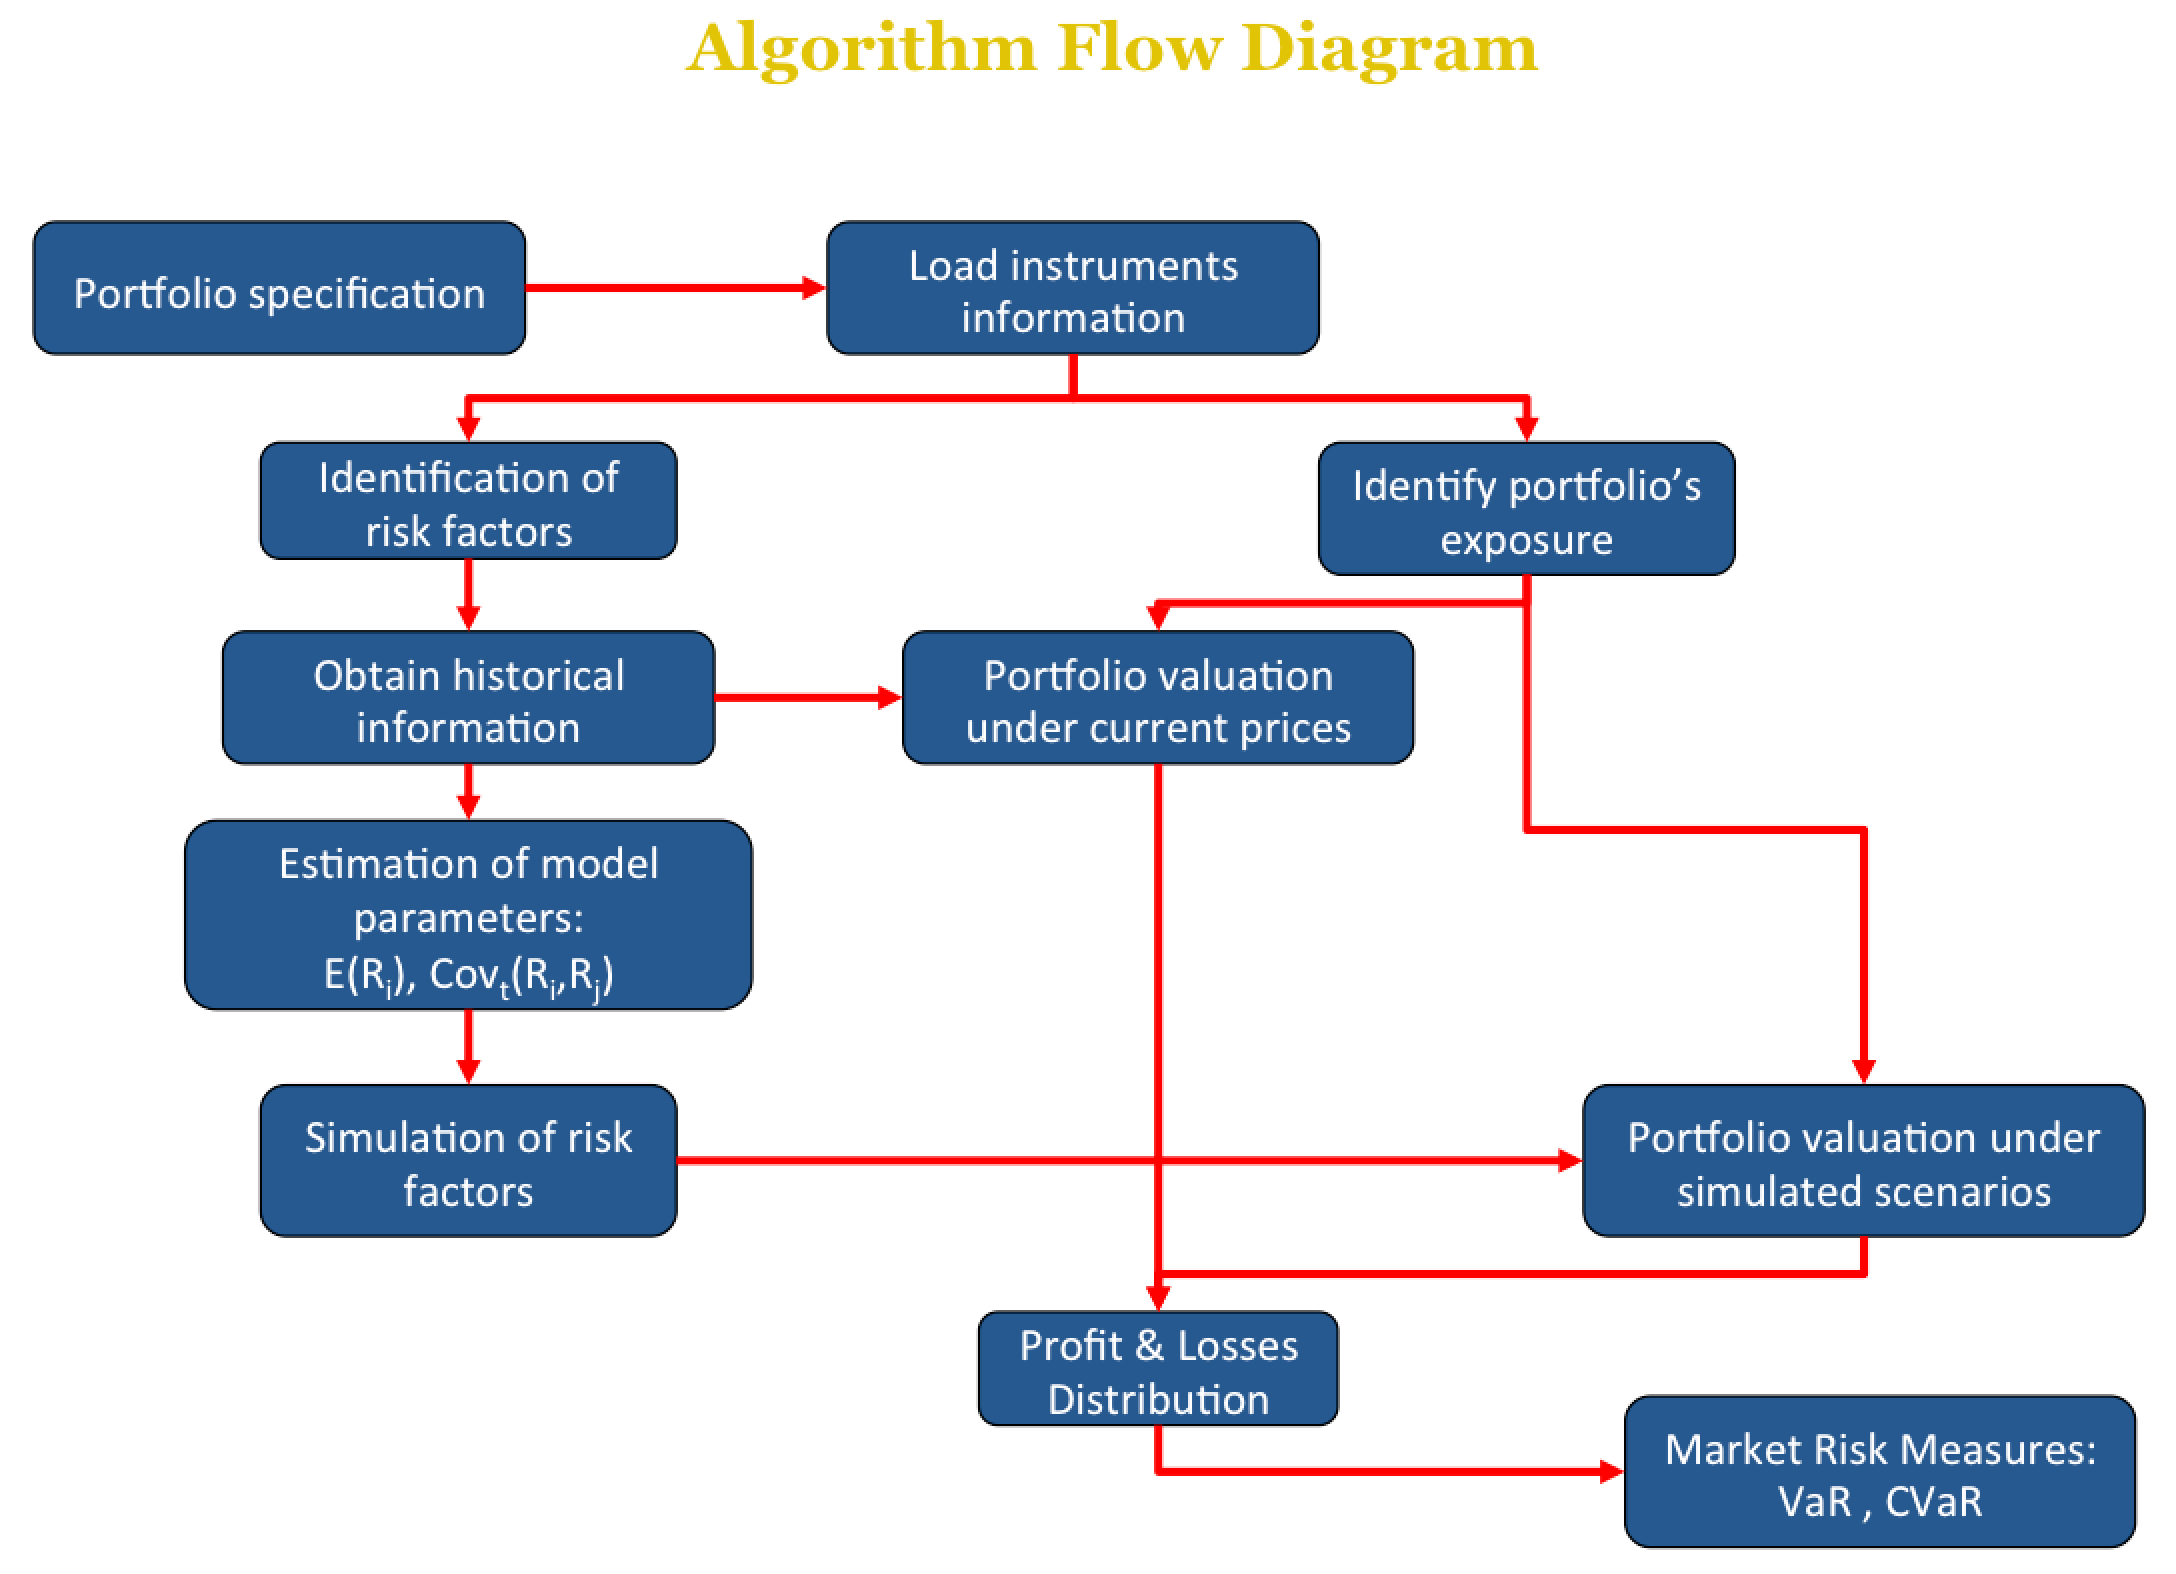
\includegraphics[max size={\textwidth}{\textheight}]{Market Risk Calculation_files/Market Risk Calculation_4_0.png}
    \par
    \end{center}
    
            \end{InvisibleVerbatim}
            
        
    
\section{GitHub project repository}I developed this project using Github for version control and for
storing all the files required to run this algorithm as well as
additional documentation regarding market risk.

This repository can be found in the following address:

https://github.com/christianu7/stat\_222\_chris\_carmona\part{Parameter definition}

    % Make sure that atleast 4 lines are below the HR
    \needspace{4\baselineskip}

    
        \vspace{6pt}
        \makebox[0.1\linewidth]{\smaller\hfill\tt\color{nbframe-in-prompt}In\hspace{4pt}{[}5{]}:\hspace{4pt}}\\*
        \vspace{-2.65\baselineskip}
        \begin{ColorVerbatim}
            \vspace{-0.7\baselineskip}
            \begin{Verbatim}[commandchars=\\\{\}]
\PY{c}{\PYZsh{} FOR READING and SAVING THE DATASETS IN THE SPECIFIED DIRECTORY \PYZsh{}}
\PY{n}{data\PYZus{}dir} \PY{o}{=} \PY{l+s}{\PYZsq{}}\PY{l+s}{/Users/Chris/Documents/26 UC Berkeley/03 Courses/STAT 222/stat\PYZus{}222\PYZus{}chris\PYZus{}carmona/data/}\PY{l+s}{\PYZsq{}}

\PY{c}{\PYZsh{} FOR SAVING THE RESULTS IN THE SPECIFIED DIRECTORY \PYZsh{}}
\PY{n}{out\PYZus{}dir} \PY{o}{=} \PY{l+s}{\PYZsq{}}\PY{l+s}{/Users/Chris/Documents/26 UC Berkeley/03 Courses/STAT 222/stat\PYZus{}222\PYZus{}chris\PYZus{}carmona/output/}\PY{l+s}{\PYZsq{}}

\PY{c}{\PYZsh{} Portfolio file \PYZsh{}}
\PY{n}{port\PYZus{}file} \PY{o}{=} \PY{l+s}{\PYZsq{}}\PY{l+s}{port\PYZus{}2013\PYZhy{}12.csv}\PY{l+s}{\PYZsq{}}

\PY{c}{\PYZsh{} Date of Calculation \PYZsh{}}
\PY{n}{calc\PYZus{}date} \PY{o}{=} \PY{l+s}{\PYZsq{}}\PY{l+s}{2013\PYZhy{}12\PYZhy{}30}\PY{l+s}{\PYZsq{}}
\PY{n}{calc\PYZus{}date} \PY{o}{=} \PY{n}{datetime}\PY{o}{.}\PY{n}{strptime}\PY{p}{(}\PY{n}{calc\PYZus{}date}\PY{p}{,}\PY{l+s}{\PYZsq{}}\PY{l+s}{\PYZpc{}}\PY{l+s}{Y\PYZhy{}}\PY{l+s}{\PYZpc{}}\PY{l+s}{m\PYZhy{}}\PY{l+s+si}{\PYZpc{}d}\PY{l+s}{\PYZsq{}}\PY{p}{)}
\end{Verbatim}

            
                \vspace{-0.2\baselineskip}
            
        \end{ColorVerbatim}
    
\part{Definition of Investment Portfolio}The portfolio is loaded from a .csv file containing two columns:

\begin{enumerate}
\def\labelenumi{\arabic{enumi}.}
\itemsep1pt\parskip0pt\parsep0pt
\item
  ID of each instrument in position
\item
  Position: depending on the instrument it can be position in foreign
  currency or face value of bond holding
\end{enumerate}

    % Make sure that atleast 4 lines are below the HR
    \needspace{4\baselineskip}

    
        \vspace{6pt}
        \makebox[0.1\linewidth]{\smaller\hfill\tt\color{nbframe-in-prompt}In\hspace{4pt}{[}3{]}:\hspace{4pt}}\\*
        \vspace{-2.65\baselineskip}
        \begin{ColorVerbatim}
            \vspace{-0.7\baselineskip}
            \begin{Verbatim}[commandchars=\\\{\}]
\PY{c}{\PYZsh{} Portfolio \PYZsh{}}
\PY{c}{\PYZsh{}port = pd.read\PYZus{}csv( data\PYZus{}dir + port\PYZus{}file , na\PYZus{}values=[\PYZsq{}\PYZsq{},\PYZsq{}NA\PYZsq{},\PYZsq{}na\PYZsq{},\PYZsq{}NaN\PYZsq{},\PYZsq{}NULL\PYZsq{}] )}
\PY{n}{port} \PY{o}{=} \PY{n}{pd}\PY{o}{.}\PY{n}{read\PYZus{}csv}\PY{p}{(} \PY{n}{data\PYZus{}dir} \PY{o}{+} \PY{n}{port\PYZus{}file} \PY{p}{,} \PY{n}{na\PYZus{}values}\PY{o}{=}\PY{p}{[}\PY{l+s}{\PYZsq{}}\PY{l+s}{\PYZsq{}}\PY{p}{,}\PY{l+s}{\PYZsq{}}\PY{l+s}{NA}\PY{l+s}{\PYZsq{}}\PY{p}{,}\PY{l+s}{\PYZsq{}}\PY{l+s}{na}\PY{l+s}{\PYZsq{}}\PY{p}{,}\PY{l+s}{\PYZsq{}}\PY{l+s}{NaN}\PY{l+s}{\PYZsq{}}\PY{p}{,}\PY{l+s}{\PYZsq{}}\PY{l+s}{NULL}\PY{l+s}{\PYZsq{}}\PY{p}{]} \PY{p}{)}

\PY{n}{port} \PY{o}{=} \PY{n}{pd}\PY{o}{.}\PY{n}{Series}\PY{p}{(}\PY{n}{port}\PY{o}{.}\PY{n}{position}\PY{o}{.}\PY{n}{values}\PY{p}{,}\PY{n}{index}\PY{o}{=}\PY{n}{port}\PY{o}{.}\PY{n}{id\PYZus{}instr}\PY{p}{)}
\PY{n}{port}
\end{Verbatim}

            
                \vspace{-0.2\baselineskip}
            
        \end{ColorVerbatim}
    

    

        % If the first block is an image, minipage the image.  Else
        % request a certain amount of space for the input text.
        \needspace{4\baselineskip}
        
        

            % Add document contents.
            
                \makebox[0.1\linewidth]{\smaller\hfill\tt\color{nbframe-out-prompt}Out\hspace{4pt}{[}3{]}:\hspace{4pt}}\\*
                \vspace{-2.55\baselineskip}\begin{InvisibleVerbatim}
                \vspace{-0.5\baselineskip}
\begin{alltt}id\_instr
USD              1000000
CAD               900000
EUR              7000000
JPY             99000000
US912796AQ20       85001
US912796AR03       83002
US912796AW97       50001
US912796BA68       50001
US912796BE80       53002
US912796BJ77       53001
US912796BP38       25000
US912796BS76       50002
US912796BT59       25001
US912796BU23       60001
US912796BV06       60001
\ldots
CA135087ZC17     9000.0
CA135087ZF48    11341.7
CA135087ZL16     9900.0
CA135087ZN71     7991.7
CA135087ZQ03    10500.0
CA135087ZR85    10816.2
CA135087ZW70     8732.3
CA135087ZX53    15600.0
CA135087ZY37     7973.7
CA135087A388    15300.0
CA135087A537     8639.2
CA135087A792    14700.0
CA135087A958     9900.0
CA135087B295     8100.0
CA135087B527     9900.0
Length: 383, dtype: float64\end{alltt}

            \end{InvisibleVerbatim}
            
        
    
\part{Risk Factors historical information}\section{Historical Bond's Yield-to-Maturity Rates}\subsection{Downloading data}The historical Data of yield to maturity for US government bonds is
downloaded from the Department of treasury website.

The data is available in xml format

    % Make sure that atleast 4 lines are below the HR
    \needspace{4\baselineskip}

    
        \vspace{6pt}
        \makebox[0.1\linewidth]{\smaller\hfill\tt\color{nbframe-in-prompt}In\hspace{4pt}{[}4{]}:\hspace{4pt}}\\*
        \vspace{-2.65\baselineskip}
        \begin{ColorVerbatim}
            \vspace{-0.7\baselineskip}
            \begin{Verbatim}[commandchars=\\\{\}]
\PY{k}{for} \PY{n}{year} \PY{o+ow}{in} \PY{n+nb}{range}\PY{p}{(}\PY{l+m+mi}{2005}\PY{p}{,}\PY{l+m+mi}{2015}\PY{p}{)}\PY{p}{:}
    \PY{n}{url} \PY{o}{=} \PY{l+s}{\PYZsq{}}\PY{l+s}{http://www.treasury.gov/resource\PYZhy{}center/data\PYZhy{}chart\PYZhy{}center/interest\PYZhy{}rates/pages/XmlView.aspx?data=yieldyear\PYZam{}year=}\PY{l+s}{\PYZsq{}} \PY{o}{+} \PY{n+nb}{str}\PY{p}{(}\PY{n}{year}\PY{p}{)}
    \PY{n}{urllib}\PY{o}{.}\PY{n}{urlretrieve}\PY{p}{(}\PY{n}{url}\PY{p}{,} \PY{n}{data\PYZus{}dir}\PY{o}{+}\PY{l+s}{\PYZdq{}}\PY{l+s}{yields\PYZus{}}\PY{l+s}{\PYZdq{}}\PY{o}{+}\PY{n+nb}{str}\PY{p}{(}\PY{n}{year}\PY{p}{)}\PY{o}{+}\PY{l+s}{\PYZdq{}}\PY{l+s}{.xml}\PY{l+s}{\PYZdq{}}\PY{p}{)}
\end{Verbatim}

            
                \vspace{-0.2\baselineskip}
            
        \end{ColorVerbatim}
    
\subsection{Reading data}For reading the data from the xml files I used the modile `lxml' and
`etree'

In this case, the data was stored in the `text' property of a deeply
nested label.

This process dive into the levels of the xml, reads the data and finally
creates a csv file with the cleaned data.

    % Make sure that atleast 4 lines are below the HR
    \needspace{4\baselineskip}

    
        \vspace{6pt}
        \makebox[0.1\linewidth]{\smaller\hfill\tt\color{nbframe-in-prompt}In\hspace{4pt}{[}5{]}:\hspace{4pt}}\\*
        \vspace{-2.65\baselineskip}
        \begin{ColorVerbatim}
            \vspace{-0.7\baselineskip}
            \begin{Verbatim}[commandchars=\\\{\}]
\PY{n}{nodes\PYZus{}names} \PY{o}{=} \PY{p}{[}\PY{l+s}{\PYZsq{}}\PY{l+s}{GOVT\PYZus{}USD\PYZus{}USA\PYZus{}1m}\PY{l+s}{\PYZsq{}}\PY{p}{,}\PY{l+s}{\PYZsq{}}\PY{l+s}{GOVT\PYZus{}USD\PYZus{}USA\PYZus{}3m}\PY{l+s}{\PYZsq{}}\PY{p}{,}\PY{l+s}{\PYZsq{}}\PY{l+s}{GOVT\PYZus{}USD\PYZus{}USA\PYZus{}6m}\PY{l+s}{\PYZsq{}}\PY{p}{,}
               \PY{l+s}{\PYZsq{}}\PY{l+s}{GOVT\PYZus{}USD\PYZus{}USA\PYZus{}1y}\PY{l+s}{\PYZsq{}}\PY{p}{,}\PY{l+s}{\PYZsq{}}\PY{l+s}{GOVT\PYZus{}USD\PYZus{}USA\PYZus{}2y}\PY{l+s}{\PYZsq{}}\PY{p}{,}\PY{l+s}{\PYZsq{}}\PY{l+s}{GOVT\PYZus{}USD\PYZus{}USA\PYZus{}3y}\PY{l+s}{\PYZsq{}}\PY{p}{,}
               \PY{l+s}{\PYZsq{}}\PY{l+s}{GOVT\PYZus{}USD\PYZus{}USA\PYZus{}5y}\PY{l+s}{\PYZsq{}}\PY{p}{,}\PY{l+s}{\PYZsq{}}\PY{l+s}{GOVT\PYZus{}USD\PYZus{}USA\PYZus{}7y}\PY{l+s}{\PYZsq{}}\PY{p}{,}\PY{l+s}{\PYZsq{}}\PY{l+s}{GOVT\PYZus{}USD\PYZus{}USA\PYZus{}10y}\PY{l+s}{\PYZsq{}}\PY{p}{,}
               \PY{l+s}{\PYZsq{}}\PY{l+s}{GOVT\PYZus{}USD\PYZus{}USA\PYZus{}20y}\PY{l+s}{\PYZsq{}}\PY{p}{,}\PY{l+s}{\PYZsq{}}\PY{l+s}{GOVT\PYZus{}USD\PYZus{}USA\PYZus{}30y}\PY{l+s}{\PYZsq{}}\PY{p}{]}
\PY{n}{nodes\PYZus{}names\PYZus{}xml} \PY{o}{=} \PY{p}{[}\PY{l+s}{\PYZsq{}}\PY{l+s}{BC\PYZus{}1MONTH}\PY{l+s}{\PYZsq{}}\PY{p}{,}\PY{l+s}{\PYZsq{}}\PY{l+s}{BC\PYZus{}3MONTH}\PY{l+s}{\PYZsq{}}\PY{p}{,}\PY{l+s}{\PYZsq{}}\PY{l+s}{BC\PYZus{}6MONTH}\PY{l+s}{\PYZsq{}}\PY{p}{,}
                   \PY{l+s}{\PYZsq{}}\PY{l+s}{BC\PYZus{}1YEAR}\PY{l+s}{\PYZsq{}}\PY{p}{,}\PY{l+s}{\PYZsq{}}\PY{l+s}{BC\PYZus{}2YEAR}\PY{l+s}{\PYZsq{}}\PY{p}{,}\PY{l+s}{\PYZsq{}}\PY{l+s}{BC\PYZus{}3YEAR}\PY{l+s}{\PYZsq{}}\PY{p}{,}
                   \PY{l+s}{\PYZsq{}}\PY{l+s}{BC\PYZus{}5YEAR}\PY{l+s}{\PYZsq{}}\PY{p}{,}\PY{l+s}{\PYZsq{}}\PY{l+s}{BC\PYZus{}7YEAR}\PY{l+s}{\PYZsq{}}\PY{p}{,}\PY{l+s}{\PYZsq{}}\PY{l+s}{BC\PYZus{}10YEAR}\PY{l+s}{\PYZsq{}}\PY{p}{,}
                   \PY{l+s}{\PYZsq{}}\PY{l+s}{BC\PYZus{}20YEAR}\PY{l+s}{\PYZsq{}}\PY{p}{,}\PY{l+s}{\PYZsq{}}\PY{l+s}{BC\PYZus{}30YEAR}\PY{l+s}{\PYZsq{}}\PY{p}{]}
    
\PY{c}{\PYZsh{}\PYZsh{}\PYZsh{}\PYZsh{}\PYZsh{} Loading xml file \PYZsh{}\PYZsh{}\PYZsh{}\PYZsh{}\PYZsh{}}

\PY{k}{def} \PY{n+nf}{read\PYZus{}yields\PYZus{}xml}\PY{p}{(}\PY{n}{xml\PYZus{}file}\PY{p}{,}\PY{n}{nodes\PYZus{}names}\PY{p}{,}\PY{n}{nodes\PYZus{}names\PYZus{}xml}\PY{p}{)}\PY{p}{:}
    \PY{n}{doc} \PY{o}{=} \PY{n}{etree}\PY{o}{.}\PY{n}{parse}\PY{p}{(}\PY{n}{xml\PYZus{}file}\PY{p}{)}
    \PY{c}{\PYZsh{} root element: 254 elements}
    \PY{n}{root} \PY{o}{=} \PY{n}{doc}\PY{o}{.}\PY{n}{getroot}\PY{p}{(}\PY{p}{)}
    
    \PY{n}{rates\PYZus{}data} \PY{o}{=} \PY{p}{\PYZob{}}\PY{p}{\PYZcb{}}
    \PY{k}{for} \PY{n}{entries} \PY{o+ow}{in} \PY{n}{root}\PY{o}{.}\PY{n}{findall}\PY{p}{(}\PY{l+s}{\PYZsq{}}\PY{l+s}{\PYZob{}http://www.w3.org/2005/Atom\PYZcb{}entry}\PY{l+s}{\PYZsq{}}\PY{p}{)}\PY{p}{:}    
        \PY{k}{for} \PY{n}{content\PYZus{}i} \PY{o+ow}{in} \PY{n}{entries}\PY{o}{.}\PY{n}{find}\PY{p}{(}\PY{l+s}{\PYZsq{}}\PY{l+s}{\PYZob{}http://www.w3.org/2005/Atom\PYZcb{}content}\PY{l+s}{\PYZsq{}}\PY{p}{)}\PY{p}{:}
            \PY{n}{row\PYZus{}i} \PY{o}{=} \PY{p}{\PYZob{}}\PY{p}{\PYZcb{}}
            \PY{k}{for} \PY{n}{property\PYZus{}i} \PY{o+ow}{in} \PY{n}{content\PYZus{}i}\PY{o}{.}\PY{n}{getchildren}\PY{p}{(}\PY{p}{)}\PY{p}{:}
                \PY{k}{if} \PY{n}{property\PYZus{}i}\PY{o}{.}\PY{n}{tag}\PY{o}{.}\PY{n}{replace}\PY{p}{(}\PY{l+s}{\PYZsq{}}\PY{l+s}{\PYZob{}http://schemas.microsoft.com/ado/2007/08/dataservices\PYZcb{}}\PY{l+s}{\PYZsq{}}\PY{p}{,}\PY{l+s}{\PYZsq{}}\PY{l+s}{\PYZsq{}}\PY{p}{)}\PY{o}{==}\PY{l+s}{\PYZdq{}}\PY{l+s}{NEW\PYZus{}DATE}\PY{l+s}{\PYZdq{}}\PY{p}{:}
                    \PY{n}{date\PYZus{}i} \PY{o}{=} \PY{n}{property\PYZus{}i}\PY{o}{.}\PY{n}{text}\PY{o}{.}\PY{n}{replace}\PY{p}{(}\PY{l+s}{\PYZdq{}}\PY{l+s}{T00:00:00}\PY{l+s}{\PYZdq{}}\PY{p}{,}\PY{l+s}{\PYZdq{}}\PY{l+s}{\PYZdq{}}\PY{p}{)}
                \PY{k}{else}\PY{p}{:}
                    \PY{n}{row\PYZus{}i}\PY{p}{[} \PY{n}{property\PYZus{}i}\PY{o}{.}\PY{n}{tag}\PY{o}{.}\PY{n}{replace}\PY{p}{(}\PY{l+s}{\PYZsq{}}\PY{l+s}{\PYZob{}http://schemas.microsoft.com/ado/2007/08/dataservices\PYZcb{}}\PY{l+s}{\PYZsq{}}\PY{p}{,}\PY{l+s}{\PYZsq{}}\PY{l+s}{\PYZsq{}}\PY{p}{)} \PY{p}{]} \PY{o}{=} \PY{n}{property\PYZus{}i}\PY{o}{.}\PY{n}{text}
            \PY{n}{rates\PYZus{}data}\PY{p}{[}\PY{n}{date\PYZus{}i}\PY{p}{]}\PY{o}{=}\PY{n}{row\PYZus{}i}
    
    \PY{c}{\PYZsh{}DATE=pd.DataFrame(rates\PYZus{}data).NEW\PYZus{}DATE.astype(np.string\PYZus{})}
    \PY{c}{\PYZsh{}DATE=pd.to\PYZus{}datetime( DATE )}
    \PY{c}{\PYZsh{}rates\PYZus{}data = pd.DataFrame(rates\PYZus{}data,index=DATE)}
    \PY{c}{\PYZsh{}rates\PYZus{}data[:3]}
    
    \PY{n}{rates\PYZus{}data} \PY{o}{=} \PY{n}{pd}\PY{o}{.}\PY{n}{DataFrame}\PY{p}{(}\PY{n}{rates\PYZus{}data}\PY{p}{)}
    \PY{n}{rates\PYZus{}data} \PY{o}{=} \PY{n}{rates\PYZus{}data}\PY{o}{.}\PY{n}{T}
    \PY{n}{rates\PYZus{}data} \PY{o}{=} \PY{n}{rates\PYZus{}data}\PY{o}{.}\PY{n}{drop}\PY{p}{(}\PY{p}{[}\PY{l+s}{\PYZsq{}}\PY{l+s}{BC\PYZus{}30YEARDISPLAY}\PY{l+s}{\PYZsq{}}\PY{p}{,}\PY{l+s}{\PYZsq{}}\PY{l+s}{Id}\PY{l+s}{\PYZsq{}}\PY{p}{]}\PY{p}{,}\PY{n}{axis}\PY{o}{=}\PY{l+m+mi}{1}\PY{p}{)}
    \PY{n}{rates\PYZus{}data}\PY{o}{.}\PY{n}{rename}\PY{p}{(} \PY{n}{columns}\PY{o}{=}\PY{n+nb}{dict}\PY{p}{(} \PY{n+nb}{zip}\PY{p}{(}\PY{n}{nodes\PYZus{}names\PYZus{}xml}\PY{p}{,}\PY{n}{nodes\PYZus{}names}\PY{p}{)} \PY{p}{)}\PY{p}{,}
                      \PY{n}{inplace}\PY{o}{=}\PY{n+nb+bp}{True}\PY{p}{)}
    
    \PY{n}{rates\PYZus{}data} \PY{o}{=} \PY{n}{rates\PYZus{}data}\PY{o}{.}\PY{n}{convert\PYZus{}objects}\PY{p}{(}\PY{n}{convert\PYZus{}numeric}\PY{o}{=}\PY{n+nb+bp}{True}\PY{p}{)}
    \PY{n}{rates\PYZus{}data} \PY{o}{=} \PY{n}{rates\PYZus{}data}\PY{o}{.}\PY{n}{divide}\PY{p}{(}\PY{l+m+mi}{100}\PY{p}{)}
    \PY{n}{rates\PYZus{}data} \PY{o}{=} \PY{n}{rates\PYZus{}data}\PY{p}{[}\PY{n}{nodes\PYZus{}names}\PY{p}{]}
    
    \PY{n}{rates\PYZus{}data} \PY{o}{=} \PY{n}{rates\PYZus{}data}\PY{o}{.}\PY{n}{reindex}\PY{p}{(}\PY{n}{index}\PY{o}{=}\PY{n}{pd}\PY{o}{.}\PY{n}{to\PYZus{}datetime}\PY{p}{(}\PY{n}{rates\PYZus{}data}\PY{o}{.}\PY{n}{index}\PY{p}{)}\PY{p}{)}
    \PY{k}{return} \PY{n}{rates\PYZus{}data}

\PY{n}{yields\PYZus{}data} \PY{o}{=} \PY{n}{pd}\PY{o}{.}\PY{n}{DataFrame}\PY{p}{(}\PY{p}{)}
\PY{k}{for} \PY{n}{year} \PY{o+ow}{in} \PY{n+nb}{range}\PY{p}{(}\PY{l+m+mi}{2005}\PY{p}{,}\PY{l+m+mi}{2015}\PY{p}{)}\PY{p}{:}
    \PY{n}{xml\PYZus{}file} \PY{o}{=} \PY{n}{data\PYZus{}dir} \PY{o}{+} \PY{l+s}{\PYZdq{}}\PY{l+s}{yields\PYZus{}}\PY{l+s}{\PYZdq{}} \PY{o}{+} \PY{n+nb}{str}\PY{p}{(}\PY{n}{year}\PY{p}{)} \PY{o}{+} \PY{l+s}{\PYZdq{}}\PY{l+s}{.xml}\PY{l+s}{\PYZdq{}}
    \PY{n}{yields\PYZus{}data} \PY{o}{=} \PY{n}{pd}\PY{o}{.}\PY{n}{concat}\PY{p}{(}\PY{p}{[}\PY{n}{yields\PYZus{}data}\PY{p}{,}\PY{n}{read\PYZus{}yields\PYZus{}xml}\PY{p}{(}\PY{n}{xml\PYZus{}file}\PY{p}{,}\PY{n}{nodes\PYZus{}names}\PY{p}{,}\PY{n}{nodes\PYZus{}names\PYZus{}xml}\PY{p}{)}\PY{p}{]}\PY{p}{)}

\PY{n}{yields\PYZus{}data} \PY{o}{=} \PY{n}{yields\PYZus{}data}\PY{p}{[}\PY{n}{nodes\PYZus{}names}\PY{p}{]}
\PY{n}{yields\PYZus{}data} \PY{o}{=} \PY{n}{yields\PYZus{}data}\PY{o}{.}\PY{n}{convert\PYZus{}objects}\PY{p}{(}\PY{n}{convert\PYZus{}numeric}\PY{o}{=}\PY{n+nb+bp}{True}\PY{p}{)}

\PY{n}{yields\PYZus{}data}\PY{o}{.}\PY{n}{to\PYZus{}csv}\PY{p}{(}\PY{n}{data\PYZus{}dir}\PY{o}{+}\PY{l+s}{\PYZsq{}}\PY{l+s}{ytm\PYZus{}data.csv}\PY{l+s}{\PYZsq{}}\PY{p}{)}

\PY{n}{yields\PYZus{}data}
\end{Verbatim}

            
                \vspace{-0.2\baselineskip}
            
        \end{ColorVerbatim}
    

    

        % If the first block is an image, minipage the image.  Else
        % request a certain amount of space for the input text.
        \needspace{4\baselineskip}
        
        

            % Add document contents.
            
                \makebox[0.1\linewidth]{\smaller\hfill\tt\color{nbframe-out-prompt}Out\hspace{4pt}{[}5{]}:\hspace{4pt}}\\*
                \vspace{-2.55\baselineskip}\begin{InvisibleVerbatim}
                \vspace{-0.5\baselineskip}
\begin{alltt}<class 'pandas.core.frame.DataFrame'>
DatetimeIndex: 2327 entries, 2005-01-03 00:00:00 to 2014-04-16
00:00:00
Data columns (total 11 columns):
GOVT\_USD\_USA\_1m     2326  non-null values
GOVT\_USD\_USA\_3m     2323  non-null values
GOVT\_USD\_USA\_6m     2326  non-null values
GOVT\_USD\_USA\_1y     2326  non-null values
GOVT\_USD\_USA\_2y     2326  non-null values
GOVT\_USD\_USA\_3y     2326  non-null values
GOVT\_USD\_USA\_5y     2326  non-null values
GOVT\_USD\_USA\_7y     2326  non-null values
GOVT\_USD\_USA\_10y    2326  non-null values
GOVT\_USD\_USA\_20y    2326  non-null values
GOVT\_USD\_USA\_30y    2050  non-null values
dtypes: float64(11)\end{alltt}

            \end{InvisibleVerbatim}
            
        
    


    % Make sure that atleast 4 lines are below the HR
    \needspace{4\baselineskip}

    
        \vspace{6pt}
        \makebox[0.1\linewidth]{\smaller\hfill\tt\color{nbframe-in-prompt}In\hspace{4pt}{[}6{]}:\hspace{4pt}}\\*
        \vspace{-2.65\baselineskip}
        \begin{ColorVerbatim}
            \vspace{-0.7\baselineskip}
            \begin{Verbatim}[commandchars=\\\{\}]
\PY{c}{\PYZsh{} If you want to get a pdf with the YTM rates}
\PY{c}{\PYZsh{} Change \PYZdq{}if False:\PYZdq{} by \PYZdq{}if True:\PYZdq{}}
\PY{k}{if} \PY{n+nb+bp}{False}\PY{p}{:}    
    \PY{n}{pp} \PY{o}{=} \PY{n}{PdfPages}\PY{p}{(}\PY{n}{out\PYZus{}dir}\PY{o}{+}\PY{l+s}{\PYZsq{}}\PY{l+s}{yield\PYZus{}curves.pdf}\PY{l+s}{\PYZsq{}}\PY{p}{)}
    \PY{k}{for} \PY{n}{i} \PY{o+ow}{in} \PY{n+nb}{range}\PY{p}{(}\PY{n+nb}{len}\PY{p}{(}\PY{n}{yields\PYZus{}data}\PY{o}{.}\PY{n}{columns}\PY{p}{)}\PY{p}{)}\PY{p}{:}
        \PY{n}{plt}\PY{o}{.}\PY{n}{plot}\PY{p}{(}\PY{n}{yields\PYZus{}data}\PY{o}{.}\PY{n}{index}\PY{p}{,} \PY{n}{yields\PYZus{}data}\PY{p}{[}\PY{n}{yields\PYZus{}data}\PY{o}{.}\PY{n}{columns}\PY{p}{[}\PY{n}{i}\PY{p}{]}\PY{p}{]}\PY{p}{)}
        \PY{n}{plt}\PY{o}{.}\PY{n}{legend}\PY{p}{(}\PY{p}{[}\PY{n}{yields\PYZus{}data}\PY{o}{.}\PY{n}{columns}\PY{p}{[}\PY{n}{i}\PY{p}{]}\PY{p}{]}\PY{p}{)}
        \PY{n}{pp}\PY{o}{.}\PY{n}{savefig}\PY{p}{(}\PY{p}{)}
        \PY{n}{plt}\PY{o}{.}\PY{n}{close}\PY{p}{(}\PY{p}{)}
    \PY{n}{pp}\PY{o}{.}\PY{n}{close}\PY{p}{(}\PY{p}{)}
\end{Verbatim}

            
                \vspace{-0.2\baselineskip}
            
        \end{ColorVerbatim}
    
The following graphic shows the historical vlue of two important
interest rates: the 2 year and 10 year Yield-to-maturity.

This two rates are often compared as a benchmark for analizing the fixed
income market.

    % Make sure that atleast 4 lines are below the HR
    \needspace{4\baselineskip}

    
        \vspace{6pt}
        \makebox[0.1\linewidth]{\smaller\hfill\tt\color{nbframe-in-prompt}In\hspace{4pt}{[}7{]}:\hspace{4pt}}\\*
        \vspace{-2.65\baselineskip}
        \begin{ColorVerbatim}
            \vspace{-0.7\baselineskip}
            \begin{Verbatim}[commandchars=\\\{\}]
\PY{c}{\PYZsh{} Historical data: 2 and 10 year YTM rate }
\PY{n}{plt}\PY{o}{.}\PY{n}{plot}\PY{p}{(}\PY{n}{yields\PYZus{}data}\PY{o}{.}\PY{n}{index}\PY{p}{,} \PY{n}{yields\PYZus{}data}\PY{p}{[}\PY{l+s}{\PYZsq{}}\PY{l+s}{GOVT\PYZus{}USD\PYZus{}USA\PYZus{}2y}\PY{l+s}{\PYZsq{}}\PY{p}{]}\PY{p}{)}
\PY{n}{plt}\PY{o}{.}\PY{n}{plot}\PY{p}{(}\PY{n}{yields\PYZus{}data}\PY{o}{.}\PY{n}{index}\PY{p}{,} \PY{n}{yields\PYZus{}data}\PY{p}{[}\PY{l+s}{\PYZsq{}}\PY{l+s}{GOVT\PYZus{}USD\PYZus{}USA\PYZus{}10y}\PY{l+s}{\PYZsq{}}\PY{p}{]}\PY{p}{)}
\PY{n}{plt}\PY{o}{.}\PY{n}{ylabel}\PY{p}{(}\PY{l+s}{\PYZsq{}}\PY{l+s}{Rate (}\PY{l+s}{\PYZpc{}}\PY{l+s}{)}\PY{l+s}{\PYZsq{}}\PY{p}{)}
\PY{n}{plt}\PY{o}{.}\PY{n}{xlabel}\PY{p}{(}\PY{l+s}{\PYZsq{}}\PY{l+s}{Date}\PY{l+s}{\PYZsq{}}\PY{p}{)}
\PY{n}{plt}\PY{o}{.}\PY{n}{legend}\PY{p}{(}\PY{p}{[}\PY{l+s}{\PYZsq{}}\PY{l+s}{2y YTM rate}\PY{l+s}{\PYZsq{}}\PY{p}{,}\PY{l+s}{\PYZsq{}}\PY{l+s}{10y YTM rate}\PY{l+s}{\PYZsq{}}\PY{p}{]}\PY{p}{)}
\end{Verbatim}

            
                \vspace{-0.2\baselineskip}
            
        \end{ColorVerbatim}
    

    

        % If the first block is an image, minipage the image.  Else
        % request a certain amount of space for the input text.
        \needspace{4\baselineskip}
        
        

            % Add document contents.
            
                \makebox[0.1\linewidth]{\smaller\hfill\tt\color{nbframe-out-prompt}Out\hspace{4pt}{[}7{]}:\hspace{4pt}}\\*
                \vspace{-2.55\baselineskip}\begin{InvisibleVerbatim}
                \vspace{-0.5\baselineskip}
\begin{alltt}<matplotlib.legend.Legend at 0x109c447d0>\end{alltt}

            \end{InvisibleVerbatim}
            
                \begin{InvisibleVerbatim}
                \vspace{-0.5\baselineskip}
    \begin{center}
    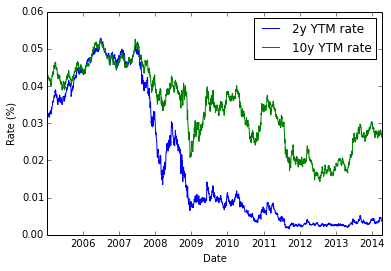
\includegraphics[max size={\textwidth}{\textheight}]{Market Risk Calculation_files/Market Risk Calculation_22_1.png}
    \par
    \end{center}
    
            \end{InvisibleVerbatim}
            
        
    
\subsection{Transform yield rates to zero-coupon rates (Bootstrap method)}This method is an iterative procedure for getting spot rates from given
prices of coupon bonds.

Suppose we have the following prices: $B_{0.5}$, $B_{1}$, $P_{1.5}$,
$P_{2}$, $P_{2.5}$, $P_{3}$, \ldots{}.

It is easy to get spot rates from zero-coupon bonds by:

$z_t = -t * log(B_t)$

for $t=0.5$ and $t=1$, we can directly obtain $z_{0.5}$ and $z_{1}$.

For $t=1.5$, we can use $P_{1.5}$ and get $B_{1.5}$ from the expression:
\[ P_{1.5} = c * (B_{0.5}+B_{1}+B_{1.5}) + B_{1.5}\] then,
\[ B_{1.5} = \frac{1}{1+c} * ( P_{1.5} - c * (B_{0.5}+B_{1})) \] which
is a zero-coupon bond, from which we can get $z_{1.5}$

this algorithm is repeated for t=\{ 1.5, 2, 2.5, 3, \ldots{} \}

    % Make sure that atleast 4 lines are below the HR
    \needspace{4\baselineskip}

    
        \vspace{6pt}
        \makebox[0.1\linewidth]{\smaller\hfill\tt\color{nbframe-in-prompt}In\hspace{4pt}{[}8{]}:\hspace{4pt}}\\*
        \vspace{-2.65\baselineskip}
        \begin{ColorVerbatim}
            \vspace{-0.7\baselineskip}
            \begin{Verbatim}[commandchars=\\\{\}]
\PY{c}{\PYZsh{}ytm\PYZus{}curve = rates\PYZus{}data.ix[0,].values}

\PY{n}{nodes} \PY{o}{=} \PY{n}{np}\PY{o}{.}\PY{n}{array}\PY{p}{(}\PY{p}{[}\PY{l+m+mi}{1}\PY{p}{,}\PY{l+m+mi}{3}\PY{p}{,}\PY{l+m+mi}{6}\PY{p}{]}\PY{p}{,}\PY{n}{dtype}\PY{o}{=}\PY{n}{np}\PY{o}{.}\PY{n}{float64}\PY{p}{)}
\PY{n}{nodes} \PY{o}{=} \PY{n}{nodes}\PY{o}{/}\PY{l+m+mi}{12}
\PY{n}{nodes} \PY{o}{=} \PY{n}{np}\PY{o}{.}\PY{n}{append}\PY{p}{(}\PY{n}{nodes}\PY{p}{,} \PY{n}{np}\PY{o}{.}\PY{n}{array}\PY{p}{(}\PY{p}{[}\PY{l+m+mi}{1}\PY{p}{,}\PY{l+m+mi}{2}\PY{p}{,}\PY{l+m+mi}{3}\PY{p}{,}\PY{l+m+mi}{5}\PY{p}{,}\PY{l+m+mi}{7}\PY{p}{,}\PY{l+m+mi}{10}\PY{p}{,}\PY{l+m+mi}{20}\PY{p}{,}\PY{l+m+mi}{30}\PY{p}{]}\PY{p}{,}\PY{n}{dtype}\PY{o}{=}\PY{n}{np}\PY{o}{.}\PY{n}{float64}\PY{p}{)} \PY{p}{)}

\PY{k}{def} \PY{n+nf}{zero\PYZus{}from\PYZus{}yield\PYZus{}bootstrap}\PY{p}{(} \PY{n}{ytm\PYZus{}curve} \PY{p}{,} \PY{n}{nodes} \PY{p}{)}\PY{p}{:}

    \PY{n}{nodes\PYZus{}old} \PY{o}{=} \PY{n}{nodes}\PY{o}{.}\PY{n}{copy}\PY{p}{(}\PY{p}{)}
    \PY{n}{nodes} \PY{o}{=} \PY{n}{np}\PY{o}{.}\PY{n}{append}\PY{p}{(}\PY{l+m+mi}{0}\PY{p}{,}\PY{n}{nodes}\PY{p}{)}
    \PY{n}{ytm\PYZus{}curve} \PY{o}{=} \PY{n}{np}\PY{o}{.}\PY{n}{append}\PY{p}{(}\PY{l+m+mi}{0}\PY{p}{,}\PY{n}{ytm\PYZus{}curve}\PY{p}{)}
    
    \PY{n}{nodes\PYZus{}new} \PY{o}{=} \PY{n}{np}\PY{o}{.}\PY{n}{arange}\PY{p}{(}\PY{l+m+mi}{0}\PY{p}{,}\PY{n+nb}{max}\PY{p}{(}\PY{n}{nodes}\PY{p}{)}\PY{o}{+}\PY{l+m+mf}{0.5}\PY{p}{,}\PY{l+m+mf}{0.5}\PY{p}{)}
    \PY{n}{nodes\PYZus{}new} \PY{o}{=} \PY{n}{np}\PY{o}{.}\PY{n}{append}\PY{p}{(}\PY{n}{nodes}\PY{p}{,}\PY{n}{nodes\PYZus{}new}\PY{p}{)}
    \PY{n}{nodes\PYZus{}new} \PY{o}{=} \PY{n}{np}\PY{o}{.}\PY{n}{sort}\PY{p}{(}\PY{n}{nodes\PYZus{}new}\PY{p}{)}
    \PY{n}{nodes\PYZus{}new} \PY{o}{=} \PY{n}{np}\PY{o}{.}\PY{n}{unique}\PY{p}{(}\PY{n}{nodes\PYZus{}new}\PY{p}{)}
        
    \PY{n}{f} \PY{o}{=} \PY{n}{interp1d}\PY{p}{(}\PY{n}{nodes}\PY{p}{,} \PY{n}{ytm\PYZus{}curve}\PY{p}{,} \PY{n}{kind}\PY{o}{=}\PY{l+s}{\PYZsq{}}\PY{l+s}{linear}\PY{l+s}{\PYZsq{}}\PY{p}{)}
    \PY{n}{ytm\PYZus{}new} \PY{o}{=} \PY{n}{f}\PY{p}{(}\PY{n}{nodes\PYZus{}new}\PY{p}{)}
    \PY{n}{ytm\PYZus{}new}\PY{p}{[}\PY{l+m+mi}{0}\PY{p}{]}\PY{o}{=}\PY{l+m+mi}{0}
    
    \PY{n}{ytm\PYZus{}new} \PY{o}{=} \PY{n}{pd}\PY{o}{.}\PY{n}{Series}\PY{p}{(}\PY{n}{ytm\PYZus{}new}\PY{p}{,}\PY{n}{index}\PY{o}{=}\PY{n}{nodes\PYZus{}new}\PY{p}{)}
    
    \PY{n}{zero\PYZus{}new} \PY{o}{=} \PY{n}{np}\PY{o}{.}\PY{n}{zeros\PYZus{}like}\PY{p}{(}\PY{n}{ytm\PYZus{}new}\PY{p}{)}
    
    \PY{n}{nodes\PYZus{}coupon} \PY{o}{=} \PY{n}{np}\PY{o}{.}\PY{n}{in1d}\PY{p}{(}\PY{n}{nodes\PYZus{}new}\PY{p}{,}\PY{n}{np}\PY{o}{.}\PY{n}{arange}\PY{p}{(}\PY{l+m+mi}{0}\PY{p}{,}\PY{n+nb}{max}\PY{p}{(}\PY{n}{nodes}\PY{p}{)}\PY{p}{,}\PY{l+m+mf}{0.5}\PY{p}{)}\PY{o}{+}\PY{l+m+mf}{0.5}\PY{p}{)}
    
    \PY{k}{for} \PY{n}{node\PYZus{}i} \PY{o+ow}{in} \PY{n}{nodes\PYZus{}new}\PY{p}{[}\PY{n}{nodes\PYZus{}coupon}\PY{o}{==}\PY{n+nb+bp}{False}\PY{p}{]}\PY{p}{:}
        \PY{n}{zero\PYZus{}new}\PY{p}{[}\PY{n}{node\PYZus{}i}\PY{p}{]} \PY{o}{=} \PY{p}{(}\PY{l+m+mi}{1}\PY{o}{+}\PY{n}{ytm\PYZus{}new}\PY{p}{[}\PY{n}{node\PYZus{}i}\PY{p}{]}\PY{o}{*}\PY{n}{node\PYZus{}i}\PY{p}{)} \PY{o}{*}\PY{o}{*} \PY{p}{(}\PY{l+m+mi}{1}\PY{o}{/}\PY{n}{node\PYZus{}i}\PY{p}{)}\PY{o}{\PYZhy{}}\PY{l+m+mi}{1}
    \PY{n}{zero\PYZus{}new}\PY{p}{[}\PY{l+m+mi}{0}\PY{p}{]} \PY{o}{=} \PY{l+m+mi}{0}
    
    
    \PY{k}{for} \PY{n}{node\PYZus{}i} \PY{o+ow}{in} \PY{n}{nodes\PYZus{}new}\PY{p}{[}\PY{n}{nodes\PYZus{}coupon}\PY{p}{]}\PY{p}{:}
        \PY{n}{cpn\PYZus{}i} \PY{o}{=} \PY{n}{ytm\PYZus{}new}\PY{p}{[}\PY{n}{node\PYZus{}i}\PY{p}{]}\PY{o}{/}\PY{l+m+mi}{2}
        \PY{n}{zero\PYZus{}new}\PY{p}{[}\PY{n}{node\PYZus{}i}\PY{p}{]} \PY{o}{=} \PY{o}{\PYZhy{}} \PY{n}{np}\PY{o}{.}\PY{n}{log}\PY{p}{(} \PY{p}{(}\PY{l+m+mi}{1} \PY{o}{\PYZhy{}} \PY{n}{cpn\PYZus{}i} \PY{o}{*} \PY{n}{np}\PY{o}{.}\PY{n}{exp}\PY{p}{(}\PY{o}{\PYZhy{}}\PY{n}{nodes\PYZus{}new}\PY{p}{[} \PY{n}{nodes\PYZus{}new}\PY{o}{\PYZlt{}}\PY{n}{node\PYZus{}i} \PY{o}{*} \PY{n}{nodes\PYZus{}coupon} \PY{p}{]} \PY{o}{*} \PY{n}{zero\PYZus{}new}\PY{p}{[} \PY{n}{nodes\PYZus{}new}\PY{o}{\PYZlt{}}\PY{n}{node\PYZus{}i} \PY{o}{*} \PY{n}{nodes\PYZus{}coupon} \PY{p}{]}\PY{p}{)}\PY{o}{.}\PY{n}{sum}\PY{p}{(}\PY{p}{)}\PY{p}{)}\PY{o}{/}\PY{p}{(}\PY{l+m+mi}{1}\PY{o}{+}\PY{n}{cpn\PYZus{}i}\PY{p}{)} \PY{p}{)} \PY{o}{*} \PY{p}{(}\PY{l+m+mi}{1}\PY{o}{/}\PY{n}{node\PYZus{}i}\PY{p}{)}

    \PY{k}{return} \PY{n}{zero\PYZus{}new}\PY{p}{[}\PY{n}{np}\PY{o}{.}\PY{n}{in1d}\PY{p}{(}\PY{n}{nodes\PYZus{}new}\PY{p}{,}\PY{n}{nodes\PYZus{}old}\PY{p}{)}\PY{p}{]}\PY{o}{.}\PY{n}{values}
\end{Verbatim}

            
                \vspace{-0.2\baselineskip}
            
        \end{ColorVerbatim}
    
The following process obtain the zero-coupon rate for all days in the
downloaded data

    % Make sure that atleast 4 lines are below the HR
    \needspace{4\baselineskip}

    
        \vspace{6pt}
        \makebox[0.1\linewidth]{\smaller\hfill\tt\color{nbframe-in-prompt}In\hspace{4pt}{[}9{]}:\hspace{4pt}}\\*
        \vspace{-2.65\baselineskip}
        \begin{ColorVerbatim}
            \vspace{-0.7\baselineskip}
            \begin{Verbatim}[commandchars=\\\{\}]
\PY{n}{zero\PYZus{}rates\PYZus{}data} \PY{o}{=} \PY{n}{yields\PYZus{}data}\PY{o}{.}\PY{n}{copy}\PY{p}{(}\PY{p}{)}

\PY{c}{\PYZsh{}yields\PYZus{}data.apply(zero\PYZus{}from\PYZus{}yield\PYZus{}bootstrap,axis=1,nodes=nodes)}

\PY{k}{for} \PY{n}{i} \PY{o+ow}{in} \PY{n+nb}{range}\PY{p}{(}\PY{n}{yields\PYZus{}data}\PY{o}{.}\PY{n}{shape}\PY{p}{[}\PY{l+m+mi}{0}\PY{p}{]}\PY{p}{)}\PY{p}{:}
\PY{c}{\PYZsh{}    print i}
    \PY{n}{zero\PYZus{}rates\PYZus{}data}\PY{o}{.}\PY{n}{ix}\PY{p}{[}\PY{n}{i}\PY{p}{,}\PY{p}{:}\PY{p}{]} \PY{o}{=} \PY{n}{zero\PYZus{}from\PYZus{}yield\PYZus{}bootstrap}\PY{p}{(} \PY{n}{yields\PYZus{}data}\PY{o}{.}\PY{n}{ix}\PY{p}{[}\PY{n}{i}\PY{p}{,}\PY{p}{]}\PY{o}{.}\PY{n}{values}\PY{p}{,}\PY{n}{nodes} \PY{p}{)}



\PY{n}{zero\PYZus{}rates\PYZus{}data} \PY{o}{=} \PY{n}{zero\PYZus{}rates\PYZus{}data}\PY{o}{.}\PY{n}{dropna}\PY{p}{(}\PY{p}{)}

\PY{n}{zero\PYZus{}rates\PYZus{}data}\PY{o}{.}\PY{n}{to\PYZus{}csv}\PY{p}{(}\PY{n}{data\PYZus{}dir}\PY{o}{+}\PY{l+s}{\PYZsq{}}\PY{l+s}{zero\PYZus{}rates\PYZus{}data.csv}\PY{l+s}{\PYZsq{}}\PY{p}{)}

\PY{n}{zero\PYZus{}rates\PYZus{}data}
\end{Verbatim}

            
                \vspace{-0.2\baselineskip}
            
        \end{ColorVerbatim}
    

    

        % If the first block is an image, minipage the image.  Else
        % request a certain amount of space for the input text.
        \needspace{4\baselineskip}
        
        

            % Add document contents.
            
                \makebox[0.1\linewidth]{\smaller\hfill\tt\color{nbframe-out-prompt}Out\hspace{4pt}{[}9{]}:\hspace{4pt}}\\*
                \vspace{-2.55\baselineskip}\begin{InvisibleVerbatim}
                \vspace{-0.5\baselineskip}
\begin{alltt}<class 'pandas.core.frame.DataFrame'>
DatetimeIndex: 2047 entries, 2006-02-09 00:00:00 to 2014-04-16
00:00:00
Data columns (total 11 columns):
GOVT\_USD\_USA\_1m     2047  non-null values
GOVT\_USD\_USA\_3m     2047  non-null values
GOVT\_USD\_USA\_6m     2047  non-null values
GOVT\_USD\_USA\_1y     2047  non-null values
GOVT\_USD\_USA\_2y     2047  non-null values
GOVT\_USD\_USA\_3y     2047  non-null values
GOVT\_USD\_USA\_5y     2047  non-null values
GOVT\_USD\_USA\_7y     2047  non-null values
GOVT\_USD\_USA\_10y    2047  non-null values
GOVT\_USD\_USA\_20y    2047  non-null values
GOVT\_USD\_USA\_30y    2047  non-null values
dtypes: float64(11)\end{alltt}

            \end{InvisibleVerbatim}
            
        
    


    % Make sure that atleast 4 lines are below the HR
    \needspace{4\baselineskip}

    
        \vspace{6pt}
        \makebox[0.1\linewidth]{\smaller\hfill\tt\color{nbframe-in-prompt}In\hspace{4pt}{[}10{]}:\hspace{4pt}}\\*
        \vspace{-2.65\baselineskip}
        \begin{ColorVerbatim}
            \vspace{-0.7\baselineskip}
            \begin{Verbatim}[commandchars=\\\{\}]
\PY{c}{\PYZsh{} If you want to get a pdf with the historical value of zero\PYZhy{}rates}
\PY{c}{\PYZsh{} Change \PYZdq{}if False:\PYZdq{} for \PYZdq{}if True:\PYZdq{}}
\PY{k}{if} \PY{n+nb+bp}{False}\PY{p}{:}
    \PY{n}{pp} \PY{o}{=} \PY{n}{PdfPages}\PY{p}{(}\PY{n}{out\PYZus{}dir}\PY{o}{+}\PY{l+s}{\PYZsq{}}\PY{l+s}{ytm\PYZus{}to\PYZus{}zero.pdf}\PY{l+s}{\PYZsq{}}\PY{p}{)}
    \PY{k}{for} \PY{n}{i} \PY{o+ow}{in} \PY{n+nb}{range}\PY{p}{(}\PY{n+nb}{len}\PY{p}{(}\PY{n}{zero\PYZus{}rates\PYZus{}data}\PY{o}{.}\PY{n}{index}\PY{p}{)}\PY{o}{\PYZhy{}}\PY{l+m+mi}{5}\PY{p}{,}\PY{n+nb}{len}\PY{p}{(}\PY{n}{zero\PYZus{}rates\PYZus{}data}\PY{o}{.}\PY{n}{index}\PY{p}{)}\PY{p}{)}\PY{p}{:}
        \PY{n}{plt}\PY{o}{.}\PY{n}{plot}\PY{p}{(}\PY{n}{nodes}\PY{p}{,}\PY{n}{zero\PYZus{}rates\PYZus{}data}\PY{o}{.}\PY{n}{ix}\PY{p}{[}\PY{n}{i}\PY{p}{,}\PY{p}{]}\PY{p}{,}\PY{n}{nodes}\PY{p}{,}\PY{n}{yields\PYZus{}data}\PY{o}{.}\PY{n}{ix}\PY{p}{[}\PY{n}{i}\PY{p}{,}\PY{p}{]}\PY{p}{)}
        \PY{n}{plt}\PY{o}{.}\PY{n}{legend}\PY{p}{(}\PY{p}{[}\PY{l+s}{\PYZsq{}}\PY{l+s}{zero\PYZhy{}coupon continuos}\PY{l+s}{\PYZsq{}}\PY{p}{,}\PY{l+s}{\PYZsq{}}\PY{l+s}{ytm semiannual}\PY{l+s}{\PYZsq{}}\PY{p}{]}\PY{p}{)}
        \PY{n}{pp}\PY{o}{.}\PY{n}{savefig}\PY{p}{(}\PY{p}{)}
        \PY{n}{plt}\PY{o}{.}\PY{n}{close}\PY{p}{(}\PY{p}{)}
    \PY{n}{pp}\PY{o}{.}\PY{n}{close}\PY{p}{(}\PY{p}{)}
\end{Verbatim}

            
                \vspace{-0.2\baselineskip}
            
        \end{ColorVerbatim}
    
The following graph shows the difference between the two curves:

\begin{enumerate}
\def\labelenumi{\arabic{enumi}.}
\itemsep1pt\parskip0pt\parsep0pt
\item
  YTM composed semiannualy
\item
  zero-coupon continuous rate
\end{enumerate}

Both rates are equivalent, but the quotation is different

    % Make sure that atleast 4 lines are below the HR
    \needspace{4\baselineskip}

    
        \vspace{6pt}
        \makebox[0.1\linewidth]{\smaller\hfill\tt\color{nbframe-in-prompt}In\hspace{4pt}{[}11{]}:\hspace{4pt}}\\*
        \vspace{-2.65\baselineskip}
        \begin{ColorVerbatim}
            \vspace{-0.7\baselineskip}
            \begin{Verbatim}[commandchars=\\\{\}]
\PY{c}{\PYZsh{} Comparison of a zero\PYZhy{}coupon yield curve with YTM curve}
\PY{n}{i} \PY{o}{=} \PY{n+nb}{len}\PY{p}{(}\PY{n}{zero\PYZus{}rates\PYZus{}data}\PY{o}{.}\PY{n}{index}\PY{p}{)}\PY{o}{\PYZhy{}}\PY{l+m+mi}{50}
\PY{n}{plt}\PY{o}{.}\PY{n}{plot}\PY{p}{(}\PY{n}{nodes}\PY{p}{,}\PY{n}{zero\PYZus{}rates\PYZus{}data}\PY{o}{.}\PY{n}{ix}\PY{p}{[}\PY{n}{i}\PY{p}{,}\PY{p}{]}\PY{p}{,}\PY{n}{nodes}\PY{p}{,}\PY{n}{yields\PYZus{}data}\PY{o}{.}\PY{n}{ix}\PY{p}{[}\PY{n}{i}\PY{p}{,}\PY{p}{]}\PY{p}{)}
\PY{n}{plt}\PY{o}{.}\PY{n}{legend}\PY{p}{(}\PY{p}{[}\PY{l+s}{\PYZsq{}}\PY{l+s}{zero\PYZhy{}coupon continuos}\PY{l+s}{\PYZsq{}}\PY{p}{,}\PY{l+s}{\PYZsq{}}\PY{l+s}{ytm semiannual}\PY{l+s}{\PYZsq{}}\PY{p}{]}\PY{p}{)}
\PY{n}{plt}\PY{o}{.}\PY{n}{ylabel}\PY{p}{(}\PY{l+s}{\PYZsq{}}\PY{l+s}{Rate (}\PY{l+s}{\PYZpc{}}\PY{l+s}{)}\PY{l+s}{\PYZsq{}}\PY{p}{)}
\PY{n}{plt}\PY{o}{.}\PY{n}{xlabel}\PY{p}{(}\PY{l+s}{\PYZsq{}}\PY{l+s}{Term (years)}\PY{l+s}{\PYZsq{}}\PY{p}{)}
\end{Verbatim}

            
                \vspace{-0.2\baselineskip}
            
        \end{ColorVerbatim}
    

    

        % If the first block is an image, minipage the image.  Else
        % request a certain amount of space for the input text.
        \needspace{4\baselineskip}
        
        

            % Add document contents.
            
                \makebox[0.1\linewidth]{\smaller\hfill\tt\color{nbframe-out-prompt}Out\hspace{4pt}{[}11{]}:\hspace{4pt}}\\*
                \vspace{-2.55\baselineskip}\begin{InvisibleVerbatim}
                \vspace{-0.5\baselineskip}
\begin{alltt}<matplotlib.text.Text at 0x109c8a750>\end{alltt}

            \end{InvisibleVerbatim}
            
                \begin{InvisibleVerbatim}
                \vspace{-0.5\baselineskip}
    \begin{center}
    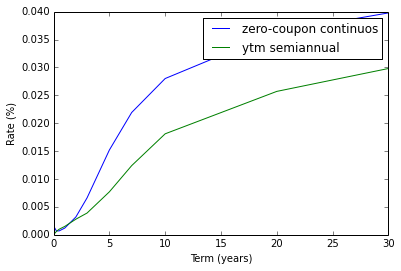
\includegraphics[max size={\textwidth}{\textheight}]{Market Risk Calculation_files/Market Risk Calculation_30_1.png}
    \par
    \end{center}
    
            \end{InvisibleVerbatim}
            
        
    
\section{Historical Foreign Exchange Rates}\subsection{Downloading data}The historical Data of Currency rates is downloaded from the Federal
Resevre website. The data is available in xml format.

    % Make sure that atleast 4 lines are below the HR
    \needspace{4\baselineskip}

    
        \vspace{6pt}
        \makebox[0.1\linewidth]{\smaller\hfill\tt\color{nbframe-in-prompt}In\hspace{4pt}{[}12{]}:\hspace{4pt}}\\*
        \vspace{-2.65\baselineskip}
        \begin{ColorVerbatim}
            \vspace{-0.7\baselineskip}
            \begin{Verbatim}[commandchars=\\\{\}]
\PY{n}{url\PYZus{}zip} \PY{o}{=} \PY{l+s}{\PYZsq{}}\PY{l+s}{http://www.federalreserve.gov/datadownload/Output.aspx?rel=H10\PYZam{}filetype=zip}\PY{l+s}{\PYZsq{}}

\PY{c}{\PYZsh{}\PYZsh{}\PYZsh{}\PYZsh{}\PYZsh{} Download zip file with data \PYZsh{}\PYZsh{}\PYZsh{}\PYZsh{}\PYZsh{}}

\PY{c}{\PYZsh{}import urllib}
\PY{n}{urllib}\PY{o}{.}\PY{n}{urlretrieve}\PY{p}{(}\PY{n}{url\PYZus{}zip}\PY{p}{,} \PY{n}{data\PYZus{}dir}\PY{o}{+}\PY{l+s}{\PYZdq{}}\PY{l+s}{ccy.zip}\PY{l+s}{\PYZdq{}}\PY{p}{)}

\PY{c}{\PYZsh{}import zipfile}
\PY{n}{zip\PYZus{}file} \PY{o}{=} \PY{n+nb}{open}\PY{p}{(}\PY{n}{data\PYZus{}dir}\PY{o}{+}\PY{l+s}{\PYZsq{}}\PY{l+s}{ccy.zip}\PY{l+s}{\PYZsq{}}\PY{p}{,} \PY{l+s}{\PYZsq{}}\PY{l+s}{rb}\PY{l+s}{\PYZsq{}}\PY{p}{)}
\PY{n}{z} \PY{o}{=} \PY{n}{zipfile}\PY{o}{.}\PY{n}{ZipFile}\PY{p}{(}\PY{n}{zip\PYZus{}file}\PY{p}{)}
\PY{c}{\PYZsh{}print z.namelist()}
\PY{n}{z}\PY{o}{.}\PY{n}{extract}\PY{p}{(}\PY{l+s}{\PYZsq{}}\PY{l+s}{H10\PYZus{}data.xml}\PY{l+s}{\PYZsq{}}\PY{p}{,} \PY{n}{data\PYZus{}dir}\PY{p}{)}
\end{Verbatim}

            
                \vspace{-0.2\baselineskip}
            
        \end{ColorVerbatim}
    

    

        % If the first block is an image, minipage the image.  Else
        % request a certain amount of space for the input text.
        \needspace{4\baselineskip}
        
        

            % Add document contents.
            
                \makebox[0.1\linewidth]{\smaller\hfill\tt\color{nbframe-out-prompt}Out\hspace{4pt}{[}12{]}:\hspace{4pt}}\\*
                \vspace{-2.55\baselineskip}\begin{InvisibleVerbatim}
                \vspace{-0.5\baselineskip}
\begin{alltt}'/Users/Chris/Documents/26 UC Berkeley/03 Courses/STAT
222/stat\_222\_chris\_carmona/data/H10\_data.xml'\end{alltt}

            \end{InvisibleVerbatim}
            
        
    
\subsection{Reading data}Equivalent to the historical data for YTM, the process for obtaining the
information consists in going deep into de different levels of the xml
format and find the important data.

In this case, the data was embeded as an attribute for the labels `Obs'

    % Make sure that atleast 4 lines are below the HR
    \needspace{4\baselineskip}

    
        \vspace{6pt}
        \makebox[0.1\linewidth]{\smaller\hfill\tt\color{nbframe-in-prompt}In\hspace{4pt}{[}13{]}:\hspace{4pt}}\\*
        \vspace{-2.65\baselineskip}
        \begin{ColorVerbatim}
            \vspace{-0.7\baselineskip}
            \begin{Verbatim}[commandchars=\\\{\}]
\PY{c}{\PYZsh{}\PYZsh{}\PYZsh{}\PYZsh{}\PYZsh{} Loading xml file \PYZsh{}\PYZsh{}\PYZsh{}\PYZsh{}\PYZsh{}}

\PY{n}{doc} \PY{o}{=} \PY{n}{etree}\PY{o}{.}\PY{n}{parse}\PY{p}{(}\PY{n}{data\PYZus{}dir}\PY{o}{+}\PY{l+s}{\PYZsq{}}\PY{l+s}{H10\PYZus{}data.xml}\PY{l+s}{\PYZsq{}}\PY{p}{)}
\PY{c}{\PYZsh{} root element: 254 elements}
\PY{n}{root} \PY{o}{=} \PY{n}{doc}\PY{o}{.}\PY{n}{getroot}\PY{p}{(}\PY{p}{)}

\PY{n}{data\PYZus{}set} \PY{o}{=} \PY{n}{root}\PY{o}{.}\PY{n}{find}\PY{p}{(}\PY{l+s}{\PYZsq{}}\PY{l+s}{\PYZob{}http://www.federalreserve.gov/structure/compact/common\PYZcb{}DataSet}\PY{l+s}{\PYZsq{}}\PY{p}{)}
\PY{n}{series} \PY{o}{=} \PY{n}{data\PYZus{}set}\PY{o}{.}\PY{n}{findall}\PY{p}{(}\PY{l+s}{\PYZsq{}}\PY{l+s}{\PYZob{}http://www.federalreserve.gov/structure/compact/H10\PYZus{}H10\PYZcb{}Series}\PY{l+s}{\PYZsq{}}\PY{p}{)}

\PY{n}{currencies} \PY{o}{=} \PY{p}{[}\PY{l+s}{\PYZsq{}}\PY{l+s}{AUD}\PY{l+s}{\PYZsq{}}\PY{p}{,} \PY{l+s}{\PYZsq{}}\PY{l+s}{CAD}\PY{l+s}{\PYZsq{}}\PY{p}{,} \PY{l+s}{\PYZsq{}}\PY{l+s}{CHF}\PY{l+s}{\PYZsq{}}\PY{p}{,} \PY{l+s}{\PYZsq{}}\PY{l+s}{CLP}\PY{l+s}{\PYZsq{}}\PY{p}{,} \PY{l+s}{\PYZsq{}}\PY{l+s}{CNY}\PY{l+s}{\PYZsq{}}\PY{p}{,} \PY{l+s}{\PYZsq{}}\PY{l+s}{EUR}\PY{l+s}{\PYZsq{}}\PY{p}{,} \PY{l+s}{\PYZsq{}}\PY{l+s}{GBP}\PY{l+s}{\PYZsq{}}\PY{p}{,} \PY{l+s}{\PYZsq{}}\PY{l+s}{JPY}\PY{l+s}{\PYZsq{}}\PY{p}{,} \PY{l+s}{\PYZsq{}}\PY{l+s}{NOK}\PY{l+s}{\PYZsq{}}\PY{p}{,} \PY{l+s}{\PYZsq{}}\PY{l+s}{NZD}\PY{l+s}{\PYZsq{}}\PY{p}{,} \PY{l+s}{\PYZsq{}}\PY{l+s}{SEK}\PY{l+s}{\PYZsq{}}\PY{p}{,} \PY{l+s}{\PYZsq{}}\PY{l+s}{SGD}\PY{l+s}{\PYZsq{}}\PY{p}{]}

\PY{n}{ccy\PYZus{}data} \PY{o}{=} \PY{p}{\PYZob{}}\PY{p}{\PYZcb{}}
\PY{k}{for} \PY{n}{serie} \PY{o+ow}{in} \PY{n}{series}\PY{p}{:}
\PY{c}{\PYZsh{}    print serie.attrib[\PYZsq{}FX\PYZsq{}] + \PYZsq{} \PYZsq{} + serie.attrib[\PYZsq{}CURRENCY\PYZsq{}] + \PYZsq{} \PYZsq{} + serie.attrib[\PYZsq{}UNIT\PYZsq{}] + \PYZsq{} \PYZsq{} + serie.attrib[\PYZsq{}FREQ\PYZsq{}]}
    \PY{k}{if} \PY{n}{serie}\PY{o}{.}\PY{n}{attrib}\PY{p}{[}\PY{l+s}{\PYZsq{}}\PY{l+s}{FX}\PY{l+s}{\PYZsq{}}\PY{p}{]} \PY{o+ow}{in} \PY{n}{currencies} \PY{o+ow}{and} \PY{n}{serie}\PY{o}{.}\PY{n}{attrib}\PY{p}{[}\PY{l+s}{\PYZsq{}}\PY{l+s}{FREQ}\PY{l+s}{\PYZsq{}}\PY{p}{]}\PY{o}{==}\PY{l+s}{\PYZsq{}}\PY{l+s}{9}\PY{l+s}{\PYZsq{}}\PY{p}{:}
\PY{c}{\PYZsh{}        print serie.attrib[\PYZsq{}FX\PYZsq{}] + \PYZsq{} \PYZsq{} + serie.attrib[\PYZsq{}CURRENCY\PYZsq{}] + \PYZsq{} \PYZsq{} + serie.attrib[\PYZsq{}UNIT\PYZsq{}] + \PYZsq{} \PYZsq{} + serie.attrib[\PYZsq{}FREQ\PYZsq{}]}
        \PY{n}{row\PYZus{}i} \PY{o}{=} \PY{p}{\PYZob{}}\PY{p}{\PYZcb{}}
        \PY{k}{for} \PY{n}{obs} \PY{o+ow}{in} \PY{n}{serie}\PY{o}{.}\PY{n}{findall}\PY{p}{(}\PY{l+s}{\PYZsq{}}\PY{l+s}{\PYZob{}http://www.federalreserve.gov/structure/compact/common\PYZcb{}Obs}\PY{l+s}{\PYZsq{}}\PY{p}{)}\PY{p}{:}
            \PY{n}{row\PYZus{}i}\PY{p}{[} \PY{n}{obs}\PY{o}{.}\PY{n}{attrib}\PY{p}{[}\PY{l+s}{\PYZsq{}}\PY{l+s}{TIME\PYZus{}PERIOD}\PY{l+s}{\PYZsq{}}\PY{p}{]} \PY{p}{]} \PY{o}{=} \PY{n}{obs}\PY{o}{.}\PY{n}{attrib}\PY{p}{[}\PY{l+s}{\PYZsq{}}\PY{l+s}{OBS\PYZus{}VALUE}\PY{l+s}{\PYZsq{}}\PY{p}{]}
        \PY{n}{ccy\PYZus{}data}\PY{p}{[}\PY{n}{serie}\PY{o}{.}\PY{n}{attrib}\PY{p}{[}\PY{l+s}{\PYZsq{}}\PY{l+s}{FX}\PY{l+s}{\PYZsq{}}\PY{p}{]}\PY{p}{]}\PY{o}{=}\PY{n}{row\PYZus{}i}

\PY{n}{ccy\PYZus{}data} \PY{o}{=} \PY{n}{pd}\PY{o}{.}\PY{n}{DataFrame}\PY{p}{(}\PY{n}{ccy\PYZus{}data}\PY{p}{)}
\PY{n}{ccy\PYZus{}data} \PY{o}{=} \PY{n}{ccy\PYZus{}data}\PY{o}{.}\PY{n}{convert\PYZus{}objects}\PY{p}{(}\PY{n}{convert\PYZus{}numeric}\PY{o}{=}\PY{n+nb+bp}{True}\PY{p}{)}
\PY{n}{ccy\PYZus{}data}\PY{p}{[}\PY{n}{ccy\PYZus{}data}\PY{o}{==}\PY{o}{\PYZhy{}}\PY{l+m+mi}{9999}\PY{p}{]} \PY{o}{=} \PY{n+nb}{float}\PY{p}{(}\PY{l+s}{\PYZsq{}}\PY{l+s}{NaN}\PY{l+s}{\PYZsq{}}\PY{p}{)}
\PY{n}{ccy\PYZus{}data} \PY{o}{=} \PY{n}{ccy\PYZus{}data}\PY{o}{.}\PY{n}{reindex}\PY{p}{(}\PY{n}{index}\PY{o}{=}\PY{n}{pd}\PY{o}{.}\PY{n}{to\PYZus{}datetime}\PY{p}{(}\PY{n}{ccy\PYZus{}data}\PY{o}{.}\PY{n}{index}\PY{p}{)}\PY{p}{)}

\PY{n}{ccy\PYZus{}data}\PY{o}{.}\PY{n}{to\PYZus{}csv}\PY{p}{(}\PY{n}{data\PYZus{}dir}\PY{o}{+}\PY{l+s}{\PYZsq{}}\PY{l+s}{currencies\PYZus{}data.csv}\PY{l+s}{\PYZsq{}}\PY{p}{)}

\PY{n}{ccy\PYZus{}data}
\end{Verbatim}

            
                \vspace{-0.2\baselineskip}
            
        \end{ColorVerbatim}
    

    

        % If the first block is an image, minipage the image.  Else
        % request a certain amount of space for the input text.
        \needspace{4\baselineskip}
        
        

            % Add document contents.
            
                \makebox[0.1\linewidth]{\smaller\hfill\tt\color{nbframe-out-prompt}Out\hspace{4pt}{[}13{]}:\hspace{4pt}}\\*
                \vspace{-2.55\baselineskip}\begin{InvisibleVerbatim}
                \vspace{-0.5\baselineskip}
\begin{alltt}<class 'pandas.core.frame.DataFrame'>
DatetimeIndex: 11290 entries, 1971-01-04 00:00:00 to 2014-04-11
00:00:00
Data columns (total 11 columns):
AUD    10856  non-null values
CAD    10869  non-null values
CHF    10863  non-null values
CNY    8303  non-null values
EUR    3842  non-null values
GBP    10863  non-null values
JPY    10857  non-null values
NOK    10862  non-null values
NZD    10847  non-null values
SEK    10862  non-null values
SGD    8362  non-null values
dtypes: float64(11)\end{alltt}

            \end{InvisibleVerbatim}
            
        
    


    % Make sure that atleast 4 lines are below the HR
    \needspace{4\baselineskip}

    
        \vspace{6pt}
        \makebox[0.1\linewidth]{\smaller\hfill\tt\color{nbframe-in-prompt}In\hspace{4pt}{[}14{]}:\hspace{4pt}}\\*
        \vspace{-2.65\baselineskip}
        \begin{ColorVerbatim}
            \vspace{-0.7\baselineskip}
            \begin{Verbatim}[commandchars=\\\{\}]
\PY{c}{\PYZsh{} If you want to get a pdf with the historical value of currencies}
\PY{c}{\PYZsh{} Change \PYZdq{}if False:\PYZdq{} for \PYZdq{}if True:\PYZdq{}}
\PY{k}{if} \PY{n+nb+bp}{False}\PY{p}{:}
    \PY{n}{pp} \PY{o}{=} \PY{n}{PdfPages}\PY{p}{(}\PY{n}{out\PYZus{}dir}\PY{o}{+}\PY{l+s}{\PYZsq{}}\PY{l+s}{currencies.pdf}\PY{l+s}{\PYZsq{}}\PY{p}{)}
    \PY{k}{for} \PY{n}{i} \PY{o+ow}{in} \PY{n+nb}{range}\PY{p}{(}\PY{n+nb}{len}\PY{p}{(}\PY{n}{ccy\PYZus{}data}\PY{o}{.}\PY{n}{columns}\PY{p}{)}\PY{p}{)}\PY{p}{:}
        \PY{n}{plt}\PY{o}{.}\PY{n}{plot}\PY{p}{(}\PY{n}{ccy\PYZus{}data}\PY{o}{.}\PY{n}{index}\PY{p}{,} \PY{n}{ccy\PYZus{}data}\PY{p}{[}\PY{n}{ccy\PYZus{}data}\PY{o}{.}\PY{n}{columns}\PY{p}{[}\PY{n}{i}\PY{p}{]}\PY{p}{]}\PY{p}{)}
        \PY{n}{plt}\PY{o}{.}\PY{n}{legend}\PY{p}{(}\PY{p}{[}\PY{n}{ccy\PYZus{}data}\PY{o}{.}\PY{n}{columns}\PY{p}{[}\PY{n}{i}\PY{p}{]}\PY{p}{]}\PY{p}{)}
        \PY{n}{pp}\PY{o}{.}\PY{n}{savefig}\PY{p}{(}\PY{p}{)}
        \PY{n}{plt}\PY{o}{.}\PY{n}{close}\PY{p}{(}\PY{p}{)}
    \PY{n}{pp}\PY{o}{.}\PY{n}{close}\PY{p}{(}\PY{p}{)}
\PY{n}{ccy\PYZus{}data}\PY{o}{.}\PY{n}{columns}
\end{Verbatim}

            
                \vspace{-0.2\baselineskip}
            
        \end{ColorVerbatim}
    

    

        % If the first block is an image, minipage the image.  Else
        % request a certain amount of space for the input text.
        \needspace{4\baselineskip}
        
        

            % Add document contents.
            
                \makebox[0.1\linewidth]{\smaller\hfill\tt\color{nbframe-out-prompt}Out\hspace{4pt}{[}14{]}:\hspace{4pt}}\\*
                \vspace{-2.55\baselineskip}\begin{InvisibleVerbatim}
                \vspace{-0.5\baselineskip}
\begin{alltt}Index([u'AUD', u'CAD', u'CHF', u'CNY', u'EUR', u'GBP', u'JPY', u'NOK',
u'NZD', u'SEK', u'SGD'], dtype=object)\end{alltt}

            \end{InvisibleVerbatim}
            
        
    
The following graphic shows the historical levels for a couple of
foreign currencies.

    % Make sure that atleast 4 lines are below the HR
    \needspace{4\baselineskip}

    
        \vspace{6pt}
        \makebox[0.1\linewidth]{\smaller\hfill\tt\color{nbframe-in-prompt}In\hspace{4pt}{[}18{]}:\hspace{4pt}}\\*
        \vspace{-2.65\baselineskip}
        \begin{ColorVerbatim}
            \vspace{-0.7\baselineskip}
            \begin{Verbatim}[commandchars=\\\{\}]
\PY{c}{\PYZsh{} Historical data: Some currencies rates}
\PY{n}{idx} \PY{o}{=} \PY{p}{(}\PY{n}{ccy\PYZus{}data}\PY{o}{.}\PY{n}{index} \PY{o}{\PYZgt{}} \PY{n}{datetime}\PY{o}{.}\PY{n}{strptime}\PY{p}{(}\PY{l+s}{\PYZsq{}}\PY{l+s}{2003\PYZhy{}01\PYZhy{}01}\PY{l+s}{\PYZsq{}}\PY{p}{,}\PY{l+s}{\PYZsq{}}\PY{l+s}{\PYZpc{}}\PY{l+s}{Y\PYZhy{}}\PY{l+s}{\PYZpc{}}\PY{l+s}{m\PYZhy{}}\PY{l+s+si}{\PYZpc{}d}\PY{l+s}{\PYZsq{}}\PY{p}{)}\PY{p}{)}
\PY{n}{plt}\PY{o}{.}\PY{n}{plot}\PY{p}{(}\PY{n}{ccy\PYZus{}data}\PY{o}{.}\PY{n}{index}\PY{p}{[}\PY{n}{idx}\PY{p}{]}\PY{p}{,} \PY{n}{ccy\PYZus{}data}\PY{p}{[}\PY{l+s}{\PYZsq{}}\PY{l+s}{EUR}\PY{l+s}{\PYZsq{}}\PY{p}{]}\PY{p}{[}\PY{n}{idx}\PY{p}{]}\PY{p}{)}
\PY{n}{plt}\PY{o}{.}\PY{n}{plot}\PY{p}{(}\PY{n}{ccy\PYZus{}data}\PY{o}{.}\PY{n}{index}\PY{p}{[}\PY{n}{idx}\PY{p}{]}\PY{p}{,} \PY{n}{ccy\PYZus{}data}\PY{p}{[}\PY{l+s}{\PYZsq{}}\PY{l+s}{GBP}\PY{l+s}{\PYZsq{}}\PY{p}{]}\PY{p}{[}\PY{n}{idx}\PY{p}{]}\PY{p}{)}
\PY{n}{plt}\PY{o}{.}\PY{n}{ylabel}\PY{p}{(}\PY{l+s}{\PYZsq{}}\PY{l+s}{Exchange rate (ccy per USD)}\PY{l+s}{\PYZsq{}}\PY{p}{)}
\PY{n}{plt}\PY{o}{.}\PY{n}{xlabel}\PY{p}{(}\PY{l+s}{\PYZsq{}}\PY{l+s}{Date}\PY{l+s}{\PYZsq{}}\PY{p}{)}
\PY{n}{plt}\PY{o}{.}\PY{n}{legend}\PY{p}{(}\PY{p}{[}\PY{l+s}{\PYZsq{}}\PY{l+s}{EUR}\PY{l+s}{\PYZsq{}}\PY{p}{,}\PY{l+s}{\PYZsq{}}\PY{l+s}{GBP}\PY{l+s}{\PYZsq{}}\PY{p}{]}\PY{p}{)}
\end{Verbatim}

            
                \vspace{-0.2\baselineskip}
            
        \end{ColorVerbatim}
    

    

        % If the first block is an image, minipage the image.  Else
        % request a certain amount of space for the input text.
        \needspace{4\baselineskip}
        
        

            % Add document contents.
            
                \makebox[0.1\linewidth]{\smaller\hfill\tt\color{nbframe-out-prompt}Out\hspace{4pt}{[}18{]}:\hspace{4pt}}\\*
                \vspace{-2.55\baselineskip}\begin{InvisibleVerbatim}
                \vspace{-0.5\baselineskip}
\begin{alltt}<matplotlib.legend.Legend at 0x109cd3b50>\end{alltt}

            \end{InvisibleVerbatim}
            
                \begin{InvisibleVerbatim}
                \vspace{-0.5\baselineskip}
    \begin{center}
    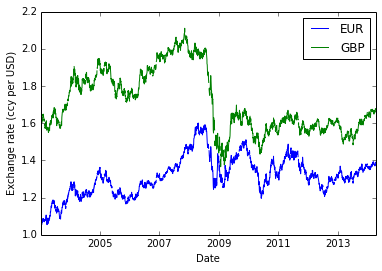
\includegraphics[max size={\textwidth}{\textheight}]{Market Risk Calculation_files/Market Risk Calculation_40_1.png}
    \par
    \end{center}
    
            \end{InvisibleVerbatim}
            
        
    
\section{Full Risk factors Information (Merging yield rates and currencies)}The following process merges the two data sources: rates and currencies

    % Make sure that atleast 4 lines are below the HR
    \needspace{4\baselineskip}

    
        \vspace{6pt}
        \makebox[0.1\linewidth]{\smaller\hfill\tt\color{nbframe-in-prompt}In\hspace{4pt}{[}19{]}:\hspace{4pt}}\\*
        \vspace{-2.65\baselineskip}
        \begin{ColorVerbatim}
            \vspace{-0.7\baselineskip}
            \begin{Verbatim}[commandchars=\\\{\}]
\PY{n}{risk\PYZus{}factors\PYZus{}hist} \PY{o}{=} \PY{n}{pd}\PY{o}{.}\PY{n}{merge}\PY{p}{(} \PY{n}{ccy\PYZus{}data}\PY{p}{,} \PY{n}{zero\PYZus{}rates\PYZus{}data}\PY{p}{,} \PY{n}{right\PYZus{}index}\PY{o}{=}\PY{n+nb+bp}{True}\PY{p}{,} \PY{n}{left\PYZus{}index}\PY{o}{=}\PY{n+nb+bp}{True}\PY{p}{,}\PY{n}{how}\PY{o}{=}\PY{l+s}{\PYZsq{}}\PY{l+s}{outer}\PY{l+s}{\PYZsq{}}\PY{p}{)}

\PY{n}{risk\PYZus{}factors\PYZus{}hist} \PY{o}{=} \PY{n}{risk\PYZus{}factors\PYZus{}hist}\PY{o}{.}\PY{n}{dropna}\PY{p}{(}\PY{p}{)}

\PY{n}{risk\PYZus{}factors\PYZus{}hist}\PY{o}{.}\PY{n}{to\PYZus{}csv}\PY{p}{(}\PY{n}{data\PYZus{}dir}\PY{o}{+}\PY{l+s}{\PYZsq{}}\PY{l+s}{factor\PYZus{}hist.csv}\PY{l+s}{\PYZsq{}}\PY{p}{)}
\PY{n}{risk\PYZus{}factors\PYZus{}hist}
\end{Verbatim}

            
                \vspace{-0.2\baselineskip}
            
        \end{ColorVerbatim}
    

    

        % If the first block is an image, minipage the image.  Else
        % request a certain amount of space for the input text.
        \needspace{4\baselineskip}
        
        

            % Add document contents.
            
                \makebox[0.1\linewidth]{\smaller\hfill\tt\color{nbframe-out-prompt}Out\hspace{4pt}{[}19{]}:\hspace{4pt}}\\*
                \vspace{-2.55\baselineskip}\begin{InvisibleVerbatim}
                \vspace{-0.5\baselineskip}
\begin{alltt}<class 'pandas.core.frame.DataFrame'>
DatetimeIndex: 2043 entries, 2006-02-09 00:00:00 to 2014-04-11
00:00:00
Data columns (total 22 columns):
AUD                 2043  non-null values
CAD                 2043  non-null values
CHF                 2043  non-null values
CNY                 2043  non-null values
EUR                 2043  non-null values
GBP                 2043  non-null values
JPY                 2043  non-null values
NOK                 2043  non-null values
NZD                 2043  non-null values
SEK                 2043  non-null values
SGD                 2043  non-null values
GOVT\_USD\_USA\_1m     2043  non-null values
GOVT\_USD\_USA\_3m     2043  non-null values
GOVT\_USD\_USA\_6m     2043  non-null values
GOVT\_USD\_USA\_1y     2043  non-null values
GOVT\_USD\_USA\_2y     2043  non-null values
GOVT\_USD\_USA\_3y     2043  non-null values
GOVT\_USD\_USA\_5y     2043  non-null values
GOVT\_USD\_USA\_7y     2043  non-null values
GOVT\_USD\_USA\_10y    2043  non-null values
GOVT\_USD\_USA\_20y    2043  non-null values
GOVT\_USD\_USA\_30y    2043  non-null values
dtypes: float64(22)\end{alltt}

            \end{InvisibleVerbatim}
            
        
    
\part{Descriptive Data bases}The following databases specify additional information for each
instrument according to their ID.

\textbf{instr\_info\_file}

Table containing the description of each instrument. i.e.~for a given
ID, specifies if the instrument is a currency position or a bond. If it
is a bond, what type of bond it is AGENCY or GOVT, and additional
information.

\textbf{cshf\_info\_file}

Table containing all cashflows for the bonds that can be part of the
portfolio. It consists of three columns: ID, date of cashflow, and
cashflow amount in USD. With one row for each cashflow date an
instrument combination.

\textbf{curves\_info\_file}

Table containing the description of the risk factors. Remember that the
risk factors are the random processes that will be stressed to valuate
the portfolio under simulated scenarios.

    % Make sure that atleast 4 lines are below the HR
    \needspace{4\baselineskip}

    
        \vspace{6pt}
        \makebox[0.1\linewidth]{\smaller\hfill\tt\color{nbframe-in-prompt}In\hspace{4pt}{[}20{]}:\hspace{4pt}}\\*
        \vspace{-2.65\baselineskip}
        \begin{ColorVerbatim}
            \vspace{-0.7\baselineskip}
            \begin{Verbatim}[commandchars=\\\{\}]
\PY{c}{\PYZsh{} Global databases \PYZsh{}}

\PY{c}{\PYZsh{} instruments description \PYZsh{}}
\PY{n}{instr\PYZus{}info\PYZus{}file} \PY{o}{=} \PY{l+s}{\PYZsq{}}\PY{l+s}{instr\PYZus{}description.csv}\PY{l+s}{\PYZsq{}}
\PY{n}{instr\PYZus{}info} \PY{o}{=} \PY{n}{pd}\PY{o}{.}\PY{n}{read\PYZus{}csv}\PY{p}{(} \PY{n}{data\PYZus{}dir} \PY{o}{+} \PY{n}{instr\PYZus{}info\PYZus{}file} \PY{p}{,} \PY{n}{na\PYZus{}values}\PY{o}{=}\PY{p}{[}\PY{l+s}{\PYZsq{}}\PY{l+s}{\PYZsq{}}\PY{p}{,}\PY{l+s}{\PYZsq{}}\PY{l+s}{NA}\PY{l+s}{\PYZsq{}}\PY{p}{,}\PY{l+s}{\PYZsq{}}\PY{l+s}{na}\PY{l+s}{\PYZsq{}}\PY{p}{,}\PY{l+s}{\PYZsq{}}\PY{l+s}{NaN}\PY{l+s}{\PYZsq{}}\PY{p}{,}\PY{l+s}{\PYZsq{}}\PY{l+s}{NULL}\PY{l+s}{\PYZsq{}}\PY{p}{]} \PY{p}{)}

\PY{c}{\PYZsh{} Risk factors description \PYZsh{}}
\PY{n}{curves\PYZus{}info\PYZus{}file} \PY{o}{=} \PY{l+s}{\PYZsq{}}\PY{l+s}{curve\PYZus{}nodes\PYZus{}description.csv}\PY{l+s}{\PYZsq{}}
\PY{n}{curves\PYZus{}info} \PY{o}{=} \PY{n}{pd}\PY{o}{.}\PY{n}{read\PYZus{}csv}\PY{p}{(} \PY{n}{data\PYZus{}dir} \PY{o}{+} \PY{n}{curves\PYZus{}info\PYZus{}file} \PY{p}{,} \PY{n}{na\PYZus{}values}\PY{o}{=}\PY{p}{[}\PY{l+s}{\PYZsq{}}\PY{l+s}{\PYZsq{}}\PY{p}{,}\PY{l+s}{\PYZsq{}}\PY{l+s}{NA}\PY{l+s}{\PYZsq{}}\PY{p}{,}\PY{l+s}{\PYZsq{}}\PY{l+s}{na}\PY{l+s}{\PYZsq{}}\PY{p}{,}\PY{l+s}{\PYZsq{}}\PY{l+s}{NaN}\PY{l+s}{\PYZsq{}}\PY{p}{,}\PY{l+s}{\PYZsq{}}\PY{l+s}{NULL}\PY{l+s}{\PYZsq{}}\PY{p}{]} \PY{p}{)}

\PY{c}{\PYZsh{} fixed\PYZhy{}income instruments cashflows \PYZsh{}}
\PY{n}{cshf\PYZus{}info\PYZus{}file} \PY{o}{=} \PY{l+s}{\PYZsq{}}\PY{l+s}{instr\PYZus{}cashflows.csv}\PY{l+s}{\PYZsq{}}
\PY{n}{cshf\PYZus{}info} \PY{o}{=} \PY{n}{pd}\PY{o}{.}\PY{n}{read\PYZus{}csv}\PY{p}{(} \PY{n}{data\PYZus{}dir} \PY{o}{+} \PY{n}{cshf\PYZus{}info\PYZus{}file} \PY{p}{,} \PY{n}{na\PYZus{}values}\PY{o}{=}\PY{p}{[}\PY{l+s}{\PYZsq{}}\PY{l+s}{\PYZsq{}}\PY{p}{,}\PY{l+s}{\PYZsq{}}\PY{l+s}{NA}\PY{l+s}{\PYZsq{}}\PY{p}{,}\PY{l+s}{\PYZsq{}}\PY{l+s}{na}\PY{l+s}{\PYZsq{}}\PY{p}{,}\PY{l+s}{\PYZsq{}}\PY{l+s}{NaN}\PY{l+s}{\PYZsq{}}\PY{p}{,}\PY{l+s}{\PYZsq{}}\PY{l+s}{NULL}\PY{l+s}{\PYZsq{}}\PY{p}{]} \PY{p}{)}
\PY{n}{cshf\PYZus{}info}\PY{p}{[}\PY{l+s}{\PYZsq{}}\PY{l+s}{Date}\PY{l+s}{\PYZsq{}}\PY{p}{]} \PY{o}{=} \PY{n}{pd}\PY{o}{.}\PY{n}{to\PYZus{}datetime}\PY{p}{(}\PY{n}{cshf\PYZus{}info}\PY{p}{[}\PY{l+s}{\PYZsq{}}\PY{l+s}{Date}\PY{l+s}{\PYZsq{}}\PY{p}{]}\PY{p}{)}
\PY{n}{cshf\PYZus{}info} \PY{o}{=} \PY{n}{cshf\PYZus{}info}\PY{o}{.}\PY{n}{groupby}\PY{p}{(}\PY{p}{[}\PY{l+s}{\PYZsq{}}\PY{l+s}{id\PYZus{}instr}\PY{l+s}{\PYZsq{}}\PY{p}{,}\PY{l+s}{\PYZsq{}}\PY{l+s}{Date}\PY{l+s}{\PYZsq{}}\PY{p}{]}\PY{p}{)}\PY{p}{[}\PY{l+s}{\PYZsq{}}\PY{l+s}{value}\PY{l+s}{\PYZsq{}}\PY{p}{]}\PY{o}{.}\PY{n}{sum}\PY{p}{(}\PY{p}{)}
\PY{c}{\PYZsh{}cshf\PYZus{}info}
\end{Verbatim}

            
                \vspace{-0.2\baselineskip}
            
        \end{ColorVerbatim}
    
\part{Risk factors scenario simulation}In the following section, we perform the simulation of risk factors.
This task requires two basic steps:

\begin{enumerate}
\def\labelenumi{\arabic{enumi}.}
\itemsep1pt\parskip0pt\parsep0pt
\item
  Estimation of the covariance matrix of risk factors using historical
  values and EWMA estimator
\item
  Simulation of returns of risk factors using the EWMA estimation and
  our geometric stochastic model.
\end{enumerate}RiskMetrics model of risk factor returns: A modified random walk
RiskMetrics methodology assumes that logarithmic returns on the risk
factors follow a multivariate normal distribution conditional on dynamic
volatility and covariances. Suppose that we have n risk factors Then,
the process generating the changes for the i-th risk factor can be
written as:
\[ \frac{dP_t^{(i)}}{P_t^{(i)}} = \mu_i dt + \sigma_i d W_t\]

where \[Var(dW^{(i)})=dt\] \[Cov(dW^{(i)},dW^{(j)})=\rho_{i,j}dt\]

It follows that the return on each asset from time t to time t+T can be
written as:
\[r_{t,T}^{(i)}=(\mu_i-\frac{1}{2}\sigma_i^2)(T-t)+\sigma_i\epsilon_i\sqrt{T-t}\]
where \[\epsilon_i \sim N(0,1)\]
\[ Cov(\epsilon_i,\epsilon_j)=\rho_{i,j} \]

If we incorporate the zero mean assumption we get that:

\[ r_{t,T}^{(i)} = \sigma_i \epsilon_i \sqrt{T-t} \]

Finally, the EWMA estimation of the covariance matrix is an estimation
that gives more importance to the more recent observations and the
importance decrease exponentially with new observations.

The parameter to control the diference in importance given to newest
observations is called `Decay factor'

The i,j entrance in the matrix is given by:
\[ \Sigma_{i,j} = \frac{1-\lambda}{1-\lambda^{m+1}}\sum\limits_{k=0}^{m} \lambda^k r_{t-k}^{(i)} r_{t-k}^{(j)} \]

where:

$m$ is the number of observations considered for calculation

$\lambda$ is the decay factor

$r_t$ risk factor return at time t\section{Calculation of Log-returns for Risk-factors}

    % Make sure that atleast 4 lines are below the HR
    \needspace{4\baselineskip}

    
        \vspace{6pt}
        \makebox[0.1\linewidth]{\smaller\hfill\tt\color{nbframe-in-prompt}In\hspace{4pt}{[}21{]}:\hspace{4pt}}\\*
        \vspace{-2.65\baselineskip}
        \begin{ColorVerbatim}
            \vspace{-0.7\baselineskip}
            \begin{Verbatim}[commandchars=\\\{\}]
\PY{c}{\PYZsh{} Flip all currencies to dollars per curency}
\PY{n}{cur\PYZus{}usd} \PY{o}{=} \PY{p}{[}\PY{l+s}{\PYZsq{}}\PY{l+s}{AUD}\PY{l+s}{\PYZsq{}}\PY{p}{,} \PY{l+s}{\PYZsq{}}\PY{l+s}{EUR}\PY{l+s}{\PYZsq{}}\PY{p}{,} \PY{l+s}{\PYZsq{}}\PY{l+s}{GBP}\PY{l+s}{\PYZsq{}}\PY{p}{,} \PY{l+s}{\PYZsq{}}\PY{l+s}{NZD}\PY{l+s}{\PYZsq{}}\PY{p}{]}
\PY{n}{cur\PYZus{}flip} \PY{o}{=} \PY{n+nb}{list}\PY{p}{(}\PY{n+nb}{set}\PY{p}{(}\PY{n}{currencies}\PY{p}{)}\PY{o}{.}\PY{n}{difference}\PY{p}{(}\PY{n+nb}{set}\PY{p}{(}\PY{n}{cur\PYZus{}usd}\PY{p}{)}\PY{p}{)}\PY{p}{)}
    
\PY{c}{\PYZsh{} Log\PYZhy{}returns calculation \PYZsh{}}
\PY{k}{def} \PY{n+nf}{get\PYZus{}logrtn}\PY{p}{(}\PY{n}{risk\PYZus{}factors\PYZus{}hist}\PY{p}{,}\PY{n}{calc\PYZus{}date}\PY{p}{,}\PY{n}{cur\PYZus{}flip}\PY{p}{)}\PY{p}{:}
    \PY{c}{\PYZsh{} only consider 1 year and half of history}
    \PY{n}{rtn\PYZus{}data} \PY{o}{=} \PY{n}{risk\PYZus{}factors\PYZus{}hist}\PY{o}{.}\PY{n}{copy}\PY{p}{(}\PY{p}{)}
    \PY{n}{rtn\PYZus{}data} \PY{o}{=} \PY{n}{rtn\PYZus{}data}\PY{p}{[} \PY{p}{(}\PY{n}{rtn\PYZus{}data}\PY{o}{.}\PY{n}{index} \PY{o}{\PYZgt{}}\PY{o}{=} \PY{n}{calc\PYZus{}date} \PY{o}{\PYZhy{}} \PY{n}{timedelta}\PY{p}{(}\PY{n}{days}\PY{o}{=}\PY{l+m+mi}{365}\PY{o}{*}\PY{l+m+mf}{1.5}\PY{o}{+}\PY{l+m+mi}{1}\PY{p}{)}\PY{p}{)} \PY{o}{\PYZam{}} \PY{p}{(}\PY{n}{rtn\PYZus{}data}\PY{o}{.}\PY{n}{index} \PY{o}{\PYZlt{}}\PY{o}{=} \PY{n}{calc\PYZus{}date} \PY{p}{)} \PY{p}{]}
    
    \PY{c}{\PYZsh{} Get rid of negative and zero values}
    \PY{n}{rtn\PYZus{}data}\PY{p}{[}\PY{n}{rtn\PYZus{}data}\PY{o}{\PYZlt{}}\PY{o}{=}\PY{l+m+mi}{0}\PY{p}{]} \PY{o}{=} \PY{n+nb}{float}\PY{p}{(}\PY{l+s}{\PYZsq{}}\PY{l+s}{NaN}\PY{l+s}{\PYZsq{}}\PY{p}{)}
    \PY{n}{rtn\PYZus{}data} \PY{o}{=} \PY{n}{rtn\PYZus{}data}\PY{o}{.}\PY{n}{dropna}\PY{p}{(}\PY{p}{)}
    
    
    \PY{c}{\PYZsh{} Flip all currencies to dollars per curency}
    \PY{k}{for} \PY{n}{cur} \PY{o+ow}{in} \PY{n}{cur\PYZus{}flip}\PY{p}{:}
        \PY{k}{if} \PY{n}{cur} \PY{o+ow}{in} \PY{n}{rtn\PYZus{}data}\PY{o}{.}\PY{n}{columns}\PY{p}{:}
            \PY{c}{\PYZsh{}print cur}
            \PY{n}{rtn\PYZus{}data}\PY{p}{[}\PY{n}{cur}\PY{p}{]} \PY{o}{=} \PY{l+m+mi}{1}\PY{o}{/}\PY{n}{rtn\PYZus{}data}\PY{p}{[}\PY{n}{cur}\PY{p}{]}
    
    \PY{c}{\PYZsh{} Calculate log\PYZhy{}returns}
    \PY{n}{rtn\PYZus{}data} \PY{o}{=} \PY{n}{rtn\PYZus{}data}\PY{o}{.}\PY{n}{apply}\PY{p}{(}\PY{n}{np}\PY{o}{.}\PY{n}{log}\PY{p}{)}
    \PY{n}{rtn\PYZus{}data} \PY{o}{=} \PY{n}{rtn\PYZus{}data} \PY{o}{\PYZhy{}} \PY{n}{rtn\PYZus{}data}\PY{o}{.}\PY{n}{shift}\PY{p}{(}\PY{l+m+mi}{1}\PY{p}{)}
    \PY{n}{rtn\PYZus{}data} \PY{o}{=} \PY{n}{rtn\PYZus{}data}\PY{o}{.}\PY{n}{dropna}\PY{p}{(}\PY{p}{)}
    \PY{n}{rtn\PYZus{}data}\PY{o}{.}\PY{n}{to\PYZus{}csv}\PY{p}{(}\PY{n}{data\PYZus{}dir}\PY{o}{+}\PY{l+s}{\PYZsq{}}\PY{l+s}{logrtn\PYZus{}data.csv}\PY{l+s}{\PYZsq{}}\PY{p}{)}
    \PY{k}{return} \PY{n}{rtn\PYZus{}data}
\end{Verbatim}

            
                \vspace{-0.2\baselineskip}
            
        \end{ColorVerbatim}
    
\section{Estimation of Risk factors Covariance matrix}

    % Make sure that atleast 4 lines are below the HR
    \needspace{4\baselineskip}

    
        \vspace{6pt}
        \makebox[0.1\linewidth]{\smaller\hfill\tt\color{nbframe-in-prompt}In\hspace{4pt}{[}{]}:\hspace{4pt}}\\*
        \vspace{-2.65\baselineskip}
        \begin{ColorVerbatim}
            \vspace{-0.7\baselineskip}
            \begin{Verbatim}[commandchars=\\\{\}]
\PY{c}{\PYZsh{} Covariance estimation:}
\PY{c}{\PYZsh{} EWMA function}
\PY{k}{def} \PY{n+nf}{ewma}\PY{p}{(} \PY{n}{X}\PY{p}{,} \PY{n}{decay} \PY{o}{=} \PY{l+m+mf}{0.96}\PY{p}{)}\PY{p}{:}
    \PY{n}{x\PYZus{}i} \PY{o}{=} \PY{n}{np}\PY{o}{.}\PY{n}{matrix}\PY{p}{(}\PY{n}{X}\PY{p}{[}\PY{l+m+mi}{0}\PY{p}{,}\PY{p}{:}\PY{p}{]}\PY{p}{)}
    \PY{n}{sigma} \PY{o}{=} \PY{n}{x\PYZus{}i}\PY{o}{.}\PY{n}{T} \PY{o}{*} \PY{n}{x\PYZus{}i}
    
    \PY{k}{for} \PY{n}{i} \PY{o+ow}{in} \PY{n+nb}{range}\PY{p}{(}\PY{l+m+mi}{1}\PY{p}{,}\PY{n}{X}\PY{o}{.}\PY{n}{shape}\PY{p}{[}\PY{l+m+mi}{0}\PY{p}{]}\PY{p}{)} \PY{p}{:}
        \PY{n}{x\PYZus{}i} \PY{o}{=} \PY{n}{np}\PY{o}{.}\PY{n}{matrix}\PY{p}{(}\PY{n}{X}\PY{p}{[}\PY{n}{i}\PY{p}{,}\PY{p}{:}\PY{p}{]}\PY{p}{)}
        \PY{n}{sigma} \PY{o}{=} \PY{n}{decay} \PY{o}{*} \PY{n}{sigma} \PY{o}{+} \PY{p}{(}\PY{l+m+mi}{1}\PY{o}{\PYZhy{}}\PY{n}{decay}\PY{p}{)} \PY{o}{*} \PY{n}{x\PYZus{}i}\PY{o}{.}\PY{n}{T} \PY{o}{*} \PY{n}{x\PYZus{}i}

    \PY{k}{return}\PY{p}{(}\PY{n}{sigma}\PY{p}{)}
\end{Verbatim}

            
                \vspace{-0.2\baselineskip}
            
        \end{ColorVerbatim}
    
\section{Function for simulation of risk factors}The function will estimate the covariance matrix for a specific day,
simulates returns according to the Multivariate geometrical brownian
model defined above, apply those returns to the quotes of risk factors
in the date, and that will provide us with simulated new quotes.

The User has to specify:

\begin{enumerate}
\def\labelenumi{\arabic{enumi}.}
\itemsep1pt\parskip0pt\parsep0pt
\item
  Number of simulations
\item
  Simulation date
\item
  Historical risk factors (a data frame with the historical information)
\item
  Currencies whose quote standard is not US dollars per currency
\item
  Decay factor for the EWMA covariance estimation
\end{enumerate}

    % Make sure that atleast 4 lines are below the HR
    \needspace{4\baselineskip}

    
        \vspace{6pt}
        \makebox[0.1\linewidth]{\smaller\hfill\tt\color{nbframe-in-prompt}In\hspace{4pt}{[}{]}:\hspace{4pt}}\\*
        \vspace{-2.65\baselineskip}
        \begin{ColorVerbatim}
            \vspace{-0.7\baselineskip}
            \begin{Verbatim}[commandchars=\\\{\}]
\PY{c}{\PYZsh{} SIMULATE RISK FACTORS \PYZsh{}}

\PY{k}{def} \PY{n+nf}{simulate\PYZus{}risk\PYZus{}factors}\PY{p}{(} \PY{n}{n\PYZus{}sim}\PY{p}{,} \PY{n}{calc\PYZus{}date}\PY{p}{,} \PY{n}{risk\PYZus{}factors\PYZus{}hist}\PY{p}{,} \PY{n}{cur\PYZus{}flip}\PY{p}{,} \PY{n}{decay}\PY{o}{=}\PY{l+m+mf}{0.96}\PY{p}{,} \PY{n}{seed}\PY{o}{=}\PY{l+m+mi}{0} \PY{p}{)}\PY{p}{:}
\PY{c}{\PYZsh{}def get\PYZus{}logrtn\PYZus{}sim( n\PYZus{}sim, calc\PYZus{}date, risk\PYZus{}factors\PYZus{}hist, decay=0.96, seed=0 ):}

    \PY{c}{\PYZsh{} Calculate log returns}
    \PY{n}{rtn\PYZus{}data} \PY{o}{=} \PY{n}{get\PYZus{}logrtn}\PY{p}{(}\PY{n}{risk\PYZus{}factors\PYZus{}hist}\PY{p}{,}\PY{n}{calc\PYZus{}date}\PY{p}{,}\PY{n}{cur\PYZus{}flip}\PY{p}{)}

    \PY{c}{\PYZsh{} Covariance matrix estimation}
    \PY{n}{sigma} \PY{o}{=} \PY{n}{ewma}\PY{p}{(} \PY{n}{rtn\PYZus{}data}\PY{o}{.}\PY{n}{values}\PY{p}{,} \PY{n}{decay}\PY{o}{=}\PY{n}{decay} \PY{p}{)}
    \PY{c}{\PYZsh{} sigma}
    
    \PY{n}{mean} \PY{o}{=} \PY{n}{np}\PY{o}{.}\PY{n}{zeros}\PY{p}{(}\PY{n}{sigma}\PY{o}{.}\PY{n}{shape}\PY{p}{[}\PY{l+m+mi}{0}\PY{p}{]}\PY{p}{)}

    \PY{c}{\PYZsh{} Generate simulated log returns}
    \PY{c}{\PYZsh{} Simulation of log\PYZhy{}returns (Multivariate Normal)}
    \PY{n}{np}\PY{o}{.}\PY{n}{random}\PY{o}{.}\PY{n}{seed}\PY{p}{(}\PY{n}{seed}\PY{o}{=}\PY{n}{seed}\PY{p}{)}
    \PY{n}{rtn\PYZus{}data\PYZus{}sim} \PY{o}{=} \PY{n}{np}\PY{o}{.}\PY{n}{random}\PY{o}{.}\PY{n}{multivariate\PYZus{}normal}\PY{p}{(} \PY{n}{mean}\PY{p}{,} \PY{n}{sigma}\PY{p}{,} \PY{n}{n\PYZus{}sim} \PY{p}{)}
    \PY{n}{rtn\PYZus{}data\PYZus{}sim} \PY{o}{=} \PY{n}{pd}\PY{o}{.}\PY{n}{DataFrame}\PY{p}{(} \PY{n}{rtn\PYZus{}data\PYZus{}sim} \PY{p}{)}
    \PY{n}{rtn\PYZus{}data\PYZus{}sim}\PY{o}{.}\PY{n}{columns} \PY{o}{=} \PY{n}{rtn\PYZus{}data}\PY{o}{.}\PY{n}{columns}
    
    \PY{c}{\PYZsh{}\PYZsh{}\PYZsh{}\PYZsh{}\PYZsh{}     Baseline scenario     \PYZsh{}\PYZsh{}\PYZsh{}\PYZsh{}\PYZsh{}}
    \PY{n}{temp} \PY{o}{=} \PY{n}{risk\PYZus{}factors\PYZus{}hist}\PY{o}{.}\PY{n}{ix}\PY{p}{[}\PY{n}{calc\PYZus{}date}\PY{p}{,}\PY{p}{]}
    \PY{n}{risk\PYZus{}factors\PYZus{}base} \PY{o}{=} \PY{n}{temp}\PY{o}{.}\PY{n}{copy}\PY{p}{(}\PY{p}{)}
    
    \PY{c}{\PYZsh{} Flip all currencies to dollars per curency}
    \PY{k}{for} \PY{n}{cur} \PY{o+ow}{in} \PY{n}{cur\PYZus{}flip}\PY{p}{:}
        \PY{k}{if} \PY{n}{cur} \PY{o+ow}{in} \PY{n}{risk\PYZus{}factors\PYZus{}base}\PY{o}{.}\PY{n}{index} \PY{p}{:}
            \PY{n}{risk\PYZus{}factors\PYZus{}base}\PY{p}{[}\PY{n}{cur}\PY{p}{]} \PY{o}{=} \PY{l+m+mi}{1}\PY{o}{/}\PY{n}{risk\PYZus{}factors\PYZus{}base}\PY{p}{[}\PY{n}{cur}\PY{p}{]}
    
    \PY{c}{\PYZsh{}\PYZsh{}\PYZsh{}\PYZsh{}\PYZsh{}     Simulated scenarios     \PYZsh{}\PYZsh{}\PYZsh{}\PYZsh{}\PYZsh{}}
    \PY{n}{risk\PYZus{}factors\PYZus{}sim} \PY{o}{=} \PY{n}{risk\PYZus{}factors\PYZus{}base} \PY{o}{*} \PY{n}{np}\PY{o}{.}\PY{n}{exp}\PY{p}{(}\PY{n}{rtn\PYZus{}data\PYZus{}sim}\PY{p}{)}
    
    \PY{c}{\PYZsh{} Flip all currencies to their original exchange standard}
    \PY{k}{for} \PY{n}{cur} \PY{o+ow}{in} \PY{n}{cur\PYZus{}flip}\PY{p}{:}
        \PY{k}{if} \PY{n}{cur} \PY{o+ow}{in} \PY{n}{risk\PYZus{}factors\PYZus{}sim}\PY{o}{.}\PY{n}{columns} \PY{p}{:}
            \PY{n}{risk\PYZus{}factors\PYZus{}sim}\PY{p}{[}\PY{n}{cur}\PY{p}{]} \PY{o}{=} \PY{l+m+mi}{1}\PY{o}{/}\PY{n}{risk\PYZus{}factors\PYZus{}sim}\PY{p}{[}\PY{n}{cur}\PY{p}{]}
            \PY{n}{risk\PYZus{}factors\PYZus{}base}\PY{p}{[}\PY{n}{cur}\PY{p}{]} \PY{o}{=} \PY{l+m+mi}{1}\PY{o}{/}\PY{n}{risk\PYZus{}factors\PYZus{}base}\PY{p}{[}\PY{n}{cur}\PY{p}{]}
    
    \PY{n}{risk\PYZus{}factors\PYZus{}sim}\PY{o}{.}\PY{n}{to\PYZus{}csv}\PY{p}{(}\PY{n}{data\PYZus{}dir}\PY{o}{+}\PY{l+s}{\PYZsq{}}\PY{l+s}{simulated\PYZus{}scenarios.csv}\PY{l+s}{\PYZsq{}}\PY{p}{)}
    \PY{n}{risk\PYZus{}factors\PYZus{}sim}

    \PY{k}{return} \PY{n}{risk\PYZus{}factors\PYZus{}sim}
\end{Verbatim}

            
                \vspace{-0.2\baselineskip}
            
        \end{ColorVerbatim}
    
\section{Obtain Simulated scenarios}

    % Make sure that atleast 4 lines are below the HR
    \needspace{4\baselineskip}

    
        \vspace{6pt}
        \makebox[0.1\linewidth]{\smaller\hfill\tt\color{nbframe-in-prompt}In\hspace{4pt}{[}22{]}:\hspace{4pt}}\\*
        \vspace{-2.65\baselineskip}
        \begin{ColorVerbatim}
            \vspace{-0.7\baselineskip}
            \begin{Verbatim}[commandchars=\\\{\}]
\PY{n}{risk\PYZus{}factors\PYZus{}sim} \PY{o}{=} \PY{n}{simulate\PYZus{}risk\PYZus{}factors}\PY{p}{(} \PY{n}{n\PYZus{}sim}\PY{o}{=}\PY{l+m+mi}{1000}\PY{p}{,}
                                         \PY{n}{calc\PYZus{}date}\PY{o}{=}\PY{n}{calc\PYZus{}date}\PY{p}{,}
                                         \PY{n}{risk\PYZus{}factors\PYZus{}hist}\PY{o}{=}\PY{n}{risk\PYZus{}factors\PYZus{}hist}\PY{p}{,}
                                         \PY{n}{cur\PYZus{}flip}\PY{o}{=}\PY{n}{cur\PYZus{}flip}\PY{p}{,} \PY{n}{decay}\PY{o}{=}\PY{l+m+mf}{0.96}\PY{p}{,} \PY{n}{seed}\PY{o}{=}\PY{l+m+mi}{0} \PY{p}{)}
\PY{n}{risk\PYZus{}factors\PYZus{}sim}
\end{Verbatim}

            
                \vspace{-0.2\baselineskip}
            
        \end{ColorVerbatim}
    

    

        % If the first block is an image, minipage the image.  Else
        % request a certain amount of space for the input text.
        \needspace{4\baselineskip}
        
        

            % Add document contents.
            
                \makebox[0.1\linewidth]{\smaller\hfill\tt\color{nbframe-out-prompt}Out\hspace{4pt}{[}22{]}:\hspace{4pt}}\\*
                \vspace{-2.55\baselineskip}\begin{InvisibleVerbatim}
                \vspace{-0.5\baselineskip}
\begin{alltt}<class 'pandas.core.frame.DataFrame'>
Int64Index: 1000 entries, 0 to 999
Data columns (total 22 columns):
AUD                 1000  non-null values
CAD                 1000  non-null values
CHF                 1000  non-null values
CNY                 1000  non-null values
EUR                 1000  non-null values
GBP                 1000  non-null values
JPY                 1000  non-null values
NOK                 1000  non-null values
NZD                 1000  non-null values
SEK                 1000  non-null values
SGD                 1000  non-null values
GOVT\_USD\_USA\_1m     1000  non-null values
GOVT\_USD\_USA\_3m     1000  non-null values
GOVT\_USD\_USA\_6m     1000  non-null values
GOVT\_USD\_USA\_1y     1000  non-null values
GOVT\_USD\_USA\_2y     1000  non-null values
GOVT\_USD\_USA\_3y     1000  non-null values
GOVT\_USD\_USA\_5y     1000  non-null values
GOVT\_USD\_USA\_7y     1000  non-null values
GOVT\_USD\_USA\_10y    1000  non-null values
GOVT\_USD\_USA\_20y    1000  non-null values
GOVT\_USD\_USA\_30y    1000  non-null values
dtypes: float64(22)\end{alltt}

            \end{InvisibleVerbatim}
            
        
    
\part{Portfolio valuation}The following section valuate the portfolio using the cashflow of each
instrument and obtaining the Financial present value.\section{Function for portfolio valuation}For a given set of

    % Make sure that atleast 4 lines are below the HR
    \needspace{4\baselineskip}

    
        \vspace{6pt}
        \makebox[0.1\linewidth]{\smaller\hfill\tt\color{nbframe-in-prompt}In\hspace{4pt}{[}23{]}:\hspace{4pt}}\\*
        \vspace{-2.65\baselineskip}
        \begin{ColorVerbatim}
            \vspace{-0.7\baselineskip}
            \begin{Verbatim}[commandchars=\\\{\}]
\PY{k}{def} \PY{n+nf}{port\PYZus{}valuation\PYZus{}slow}\PY{p}{(} \PY{n}{risk\PYZus{}factors} \PY{p}{,} \PY{n}{port}\PY{p}{,} \PY{n}{instr\PYZus{}info}\PY{p}{,} \PY{n}{cshf\PYZus{}info}\PY{p}{)}\PY{p}{:}

    \PY{n}{port\PYZus{}mtm\PYZus{}value} \PY{o}{=} \PY{n}{np}\PY{o}{.}\PY{n}{zeros\PYZus{}like}\PY{p}{(} \PY{n}{port} \PY{p}{)}
    \PY{n}{port\PYZus{}mtm\PYZus{}value}\PY{o}{.}\PY{n}{index} \PY{o}{=} \PY{n}{port}\PY{o}{.}\PY{n}{index} 
    
    \PY{c}{\PYZsh{} Discount factors calculation}
    \PY{n}{discount} \PY{o}{=} \PY{n}{pd}\PY{o}{.}\PY{n}{Series}\PY{p}{(} \PY{n}{np}\PY{o}{.}\PY{n}{array}\PY{p}{(}\PY{n}{risk\PYZus{}factors}\PY{p}{[}\PY{n}{nodes\PYZus{}names}\PY{p}{]}\PY{o}{.}\PY{n}{values}\PY{p}{)} \PY{p}{,}
                         \PY{n}{index}\PY{o}{=}\PY{p}{[} \PY{n}{calc\PYZus{}date} \PY{o}{+} \PY{n}{pd}\PY{o}{.}\PY{n}{DateOffset}\PY{p}{(}\PY{n}{days}\PY{o}{=}\PY{n}{x}\PY{o}{*}\PY{l+m+mi}{365}\PY{p}{)} \PY{k}{for} \PY{n}{x} \PY{o+ow}{in} \PY{n}{nodes} \PY{p}{]} \PY{p}{)}
    \PY{n}{discount} \PY{o}{=} \PY{n}{np}\PY{o}{.}\PY{n}{exp}\PY{p}{(}\PY{o}{\PYZhy{}}\PY{n}{discount} \PY{o}{*} \PY{n}{nodes}\PY{p}{)}
    \PY{n}{discount} \PY{o}{=} \PY{n}{discount}\PY{o}{.}\PY{n}{set\PYZus{}value}\PY{p}{(}\PY{n}{calc\PYZus{}date}\PY{p}{,} \PY{l+m+mi}{1}\PY{p}{)}
    
    \PY{k}{for} \PY{n}{instr} \PY{o+ow}{in} \PY{n}{port}\PY{o}{.}\PY{n}{index}\PY{p}{:}
        \PY{k}{if} \PY{n}{instr} \PY{o}{==} \PY{l+s}{\PYZsq{}}\PY{l+s}{USD}\PY{l+s}{\PYZsq{}}\PY{p}{:}
            \PY{n}{port\PYZus{}mtm\PYZus{}value}\PY{p}{[}\PY{n}{instr}\PY{p}{]} \PY{o}{=} \PY{n}{port}\PY{p}{[}\PY{n}{instr}\PY{p}{]}
        \PY{k}{if} \PY{n}{instr\PYZus{}info}\PY{o}{.}\PY{n}{ix}\PY{p}{[}\PY{n}{instr\PYZus{}info}\PY{o}{.}\PY{n}{id\PYZus{}instr}\PY{o}{==}\PY{n}{instr}\PY{p}{,}\PY{l+s}{\PYZdq{}}\PY{l+s}{instr\PYZus{}type\PYZus{}01}\PY{l+s}{\PYZdq{}}\PY{p}{]} \PY{o}{==} \PY{l+s}{\PYZsq{}}\PY{l+s}{CURRENCY}\PY{l+s}{\PYZsq{}} \PY{o+ow}{and} \PY{n}{instr} \PY{o}{!=} \PY{l+s}{\PYZsq{}}\PY{l+s}{USD}\PY{l+s}{\PYZsq{}}\PY{p}{:}
            \PY{k}{if} \PY{n}{instr} \PY{o+ow}{in} \PY{n}{cur\PYZus{}flip}\PY{p}{:}
                \PY{n}{port\PYZus{}mtm\PYZus{}value}\PY{p}{[}\PY{n}{instr}\PY{p}{]} \PY{o}{=} \PY{n}{port}\PY{p}{[}\PY{n}{instr}\PY{p}{]} \PY{o}{/} \PY{n}{risk\PYZus{}factors}\PY{p}{[}\PY{n}{instr}\PY{p}{]}
            \PY{k}{else}\PY{p}{:}
                \PY{n}{port\PYZus{}mtm\PYZus{}value}\PY{p}{[}\PY{n}{instr}\PY{p}{]} \PY{o}{=} \PY{n}{port}\PY{p}{[}\PY{n}{instr}\PY{p}{]} \PY{o}{*} \PY{n}{risk\PYZus{}factors}\PY{p}{[}\PY{n}{instr}\PY{p}{]}
        \PY{k}{if} \PY{n}{instr\PYZus{}info}\PY{o}{.}\PY{n}{ix}\PY{p}{[}\PY{n}{instr\PYZus{}info}\PY{o}{.}\PY{n}{id\PYZus{}instr}\PY{o}{==}\PY{n}{instr}\PY{p}{,}\PY{l+s}{\PYZdq{}}\PY{l+s}{instr\PYZus{}type\PYZus{}01}\PY{l+s}{\PYZdq{}}\PY{p}{]} \PY{o}{==} \PY{l+s}{\PYZsq{}}\PY{l+s}{BOND}\PY{l+s}{\PYZsq{}}\PY{p}{:}
            \PY{c}{\PYZsh{}print instr}
            \PY{n}{instr\PYZus{}cshf\PYZus{}dates} \PY{o}{=} \PY{n}{cshf\PYZus{}info}\PY{p}{[}\PY{n}{instr}\PY{p}{]}\PY{o}{.}\PY{n}{index}
            \PY{n}{instr\PYZus{}cshf\PYZus{}dates} \PY{o}{=} \PY{n}{instr\PYZus{}cshf\PYZus{}dates}\PY{p}{[}\PY{n}{instr\PYZus{}cshf\PYZus{}dates}\PY{o}{\PYZgt{}}\PY{o}{=}\PY{n}{calc\PYZus{}date}\PY{p}{]}
    
            \PY{n}{discount\PYZus{}1} \PY{o}{=} \PY{n}{discount}\PY{o}{.}\PY{n}{reindex}\PY{p}{(}\PY{n}{index}\PY{o}{=}\PY{n}{discount}\PY{o}{.}\PY{n}{index}\PY{o}{.}\PY{n}{append}\PY{p}{(}\PY{n}{instr\PYZus{}cshf\PYZus{}dates}\PY{p}{)}\PY{p}{)}
            \PY{n}{discount\PYZus{}1} \PY{o}{=} \PY{n}{discount\PYZus{}1}\PY{o}{.}\PY{n}{sort\PYZus{}index}\PY{p}{(}\PY{p}{)}
            \PY{n}{discount\PYZus{}1} \PY{o}{=} \PY{n}{discount\PYZus{}1}\PY{o}{.}\PY{n}{interpolate}\PY{p}{(}\PY{n}{method}\PY{o}{=}\PY{l+s}{\PYZdq{}}\PY{l+s}{time}\PY{l+s}{\PYZdq{}}\PY{p}{)}\PY{o}{.}\PY{n}{dropna}\PY{p}{(}\PY{p}{)}
    
            \PY{c}{\PYZsh{}print cshf\PYZus{}info[instr]}
            \PY{c}{\PYZsh{}print discount\PYZus{}1}
            \PY{c}{\PYZsh{}print (cshf\PYZus{}info[instr] * discount\PYZus{}1)}
    
            \PY{n}{port\PYZus{}mtm\PYZus{}value}\PY{p}{[}\PY{n}{instr}\PY{p}{]} \PY{o}{=} \PY{n+nb}{sum}\PY{p}{(} \PY{p}{(} \PY{n}{port}\PY{p}{[}\PY{n}{instr}\PY{p}{]} \PY{o}{*} \PY{p}{(}\PY{n}{cshf\PYZus{}info}\PY{p}{[}\PY{n}{instr}\PY{p}{]}\PY{o}{/}\PY{l+m+mi}{1000000}\PY{p}{)} \PY{o}{*} \PY{n}{discount\PYZus{}1} \PY{p}{)}\PY{o}{.}\PY{n}{dropna}\PY{p}{(}\PY{p}{)} \PY{p}{)}
            \PY{c}{\PYZsh{}print port\PYZus{}mtm\PYZus{}value[instr]}
            \PY{k}{if} \PY{n}{instr\PYZus{}info}\PY{o}{.}\PY{n}{ix}\PY{p}{[}\PY{n}{instr\PYZus{}info}\PY{o}{.}\PY{n}{id\PYZus{}instr}\PY{o}{==}\PY{n}{instr}\PY{p}{,}\PY{l+s}{\PYZdq{}}\PY{l+s}{currency}\PY{l+s}{\PYZdq{}}\PY{p}{]} \PY{o}{!=} \PY{l+s}{\PYZsq{}}\PY{l+s}{USD}\PY{l+s}{\PYZsq{}}\PY{p}{:}
                \PY{n}{instr\PYZus{}ccy} \PY{o}{=} \PY{n}{instr\PYZus{}info}\PY{o}{.}\PY{n}{ix}\PY{p}{[}\PY{n}{instr\PYZus{}info}\PY{o}{.}\PY{n}{id\PYZus{}instr}\PY{o}{==}\PY{n}{instr}\PY{p}{,}\PY{l+s}{\PYZdq{}}\PY{l+s}{currency}\PY{l+s}{\PYZdq{}}\PY{p}{]}
                \PY{k}{if} \PY{n}{instr\PYZus{}ccy} \PY{o+ow}{in} \PY{n}{cur\PYZus{}flip}\PY{p}{:}
                    \PY{n}{port\PYZus{}mtm\PYZus{}value}\PY{p}{[}\PY{n}{instr}\PY{p}{]} \PY{o}{=} \PY{n}{port\PYZus{}mtm\PYZus{}value}\PY{p}{[}\PY{n}{instr}\PY{p}{]} \PY{o}{/} \PY{n}{risk\PYZus{}factors}\PY{p}{[}\PY{n}{instr\PYZus{}ccy}\PY{p}{]}
                \PY{k}{else}\PY{p}{:}
                    \PY{n}{port\PYZus{}mtm\PYZus{}value}\PY{p}{[}\PY{n}{instr}\PY{p}{]} \PY{o}{=} \PY{n}{port\PYZus{}mtm\PYZus{}value}\PY{p}{[}\PY{n}{instr}\PY{p}{]} \PY{o}{*} \PY{n}{risk\PYZus{}factors}\PY{p}{[}\PY{n}{instr\PYZus{}ccy}\PY{p}{]}
    
    \PY{k}{return} \PY{n}{port\PYZus{}mtm\PYZus{}value}
\end{Verbatim}

            
                \vspace{-0.2\baselineskip}
            
        \end{ColorVerbatim}
    


    % Make sure that atleast 4 lines are below the HR
    \needspace{4\baselineskip}

    
        \vspace{6pt}
        \makebox[0.1\linewidth]{\smaller\hfill\tt\color{nbframe-in-prompt}In\hspace{4pt}{[}24{]}:\hspace{4pt}}\\*
        \vspace{-2.65\baselineskip}
        \begin{ColorVerbatim}
            \vspace{-0.7\baselineskip}
            \begin{Verbatim}[commandchars=\\\{\}]
\PY{c}{\PYZsh{}risk\PYZus{}factors = risk\PYZus{}factors\PYZus{}base.copy()}
\PY{c}{\PYZsh{}port}
\PY{c}{\PYZsh{}instr\PYZus{}info}
\PY{c}{\PYZsh{}cshf\PYZus{}info}

\PY{k}{def} \PY{n+nf}{port\PYZus{}valuation}\PY{p}{(} \PY{n}{risk\PYZus{}factors} \PY{p}{,} \PY{n}{port}\PY{p}{,} \PY{n}{instr\PYZus{}info}\PY{p}{,} \PY{n}{cshf\PYZus{}info}\PY{p}{,}\PY{n}{calc\PYZus{}date}\PY{p}{)}\PY{p}{:}
    \PY{c}{\PYZsh{} Cash flows for bonds}
    \PY{n}{bonds\PYZus{}cshf} \PY{o}{=} \PY{n}{cshf\PYZus{}info}\PY{o}{.}\PY{n}{ix}\PY{p}{[} \PY{n}{port}\PY{o}{.}\PY{n}{index}\PY{o}{.}\PY{n}{values} \PY{p}{]}\PY{o}{.}\PY{n}{unstack}\PY{p}{(}\PY{l+s}{\PYZsq{}}\PY{l+s}{id\PYZus{}instr}\PY{l+s}{\PYZsq{}}\PY{p}{)}
    \PY{n}{bonds\PYZus{}cshf} \PY{o}{=} \PY{n}{bonds\PYZus{}cshf}\PY{p}{[}\PY{n}{bonds\PYZus{}cshf}\PY{o}{.}\PY{n}{index}\PY{o}{\PYZgt{}}\PY{o}{=}\PY{n}{calc\PYZus{}date}\PY{p}{]}
    \PY{n}{bonds\PYZus{}cshf} \PY{o}{=} \PY{n}{bonds\PYZus{}cshf}\PY{o}{/}\PY{l+m+mi}{1000000}
    \PY{n}{bonds\PYZus{}cshf} \PY{o}{=} \PY{n}{bonds\PYZus{}cshf} \PY{o}{*} \PY{n}{port}\PY{p}{[}\PY{n}{bonds\PYZus{}cshf}\PY{o}{.}\PY{n}{columns}\PY{p}{]}
    
    \PY{c}{\PYZsh{} Cash flows for currencies}
    \PY{n}{ccy\PYZus{}cshf} \PY{o}{=} \PY{n}{port}\PY{p}{[}\PY{n}{currencies}\PY{p}{]}\PY{o}{.}\PY{n}{dropna}\PY{p}{(}\PY{p}{)}
    \PY{n}{ccy\PYZus{}cshf} \PY{o}{=} \PY{n}{pd}\PY{o}{.}\PY{n}{DataFrame}\PY{p}{(} \PY{n}{ccy\PYZus{}cshf}\PY{o}{.}\PY{n}{values}\PY{p}{,} \PY{n}{index}\PY{o}{=}\PY{n}{ccy\PYZus{}cshf}\PY{o}{.}\PY{n}{index}\PY{p}{,} \PY{n}{columns}\PY{o}{=}\PY{p}{[}\PY{n}{calc\PYZus{}date}\PY{p}{]} \PY{p}{)}\PY{o}{.}\PY{n}{T}
    \PY{k}{if} \PY{l+s}{\PYZsq{}}\PY{l+s}{USD}\PY{l+s}{\PYZsq{}} \PY{o+ow}{in} \PY{n}{port}\PY{o}{.}\PY{n}{index}\PY{p}{:}
        \PY{n}{ccy\PYZus{}cshf}\PY{p}{[}\PY{l+s}{\PYZsq{}}\PY{l+s}{USD}\PY{l+s}{\PYZsq{}}\PY{p}{]} \PY{o}{=} \PY{n}{port}\PY{p}{[}\PY{l+s}{\PYZsq{}}\PY{l+s}{USD}\PY{l+s}{\PYZsq{}}\PY{p}{]}
    
    \PY{c}{\PYZsh{} cashflows for all the portfolio}
    \PY{n}{port\PYZus{}cshf} \PY{o}{=} \PY{n}{pd}\PY{o}{.}\PY{n}{merge}\PY{p}{(} \PY{n}{ccy\PYZus{}cshf}\PY{p}{,} \PY{n}{bonds\PYZus{}cshf}\PY{p}{,} \PY{n}{left\PYZus{}index}\PY{o}{=}\PY{n+nb+bp}{True}\PY{p}{,} \PY{n}{right\PYZus{}index}\PY{o}{=}\PY{n+nb+bp}{True}\PY{p}{,} \PY{n}{how}\PY{o}{=}\PY{l+s}{\PYZsq{}}\PY{l+s}{outer}\PY{l+s}{\PYZsq{}} \PY{p}{)}
    \PY{n}{port\PYZus{}cshf}\PY{o}{.}\PY{n}{dropna}\PY{p}{(} \PY{n}{how}\PY{o}{=}\PY{l+s}{\PYZsq{}}\PY{l+s}{all}\PY{l+s}{\PYZsq{}} \PY{p}{)}
    
    \PY{c}{\PYZsh{} Discount factors calculation}
    \PY{n}{discount} \PY{o}{=} \PY{n}{pd}\PY{o}{.}\PY{n}{Series}\PY{p}{(} \PY{n}{np}\PY{o}{.}\PY{n}{array}\PY{p}{(}\PY{n}{risk\PYZus{}factors}\PY{p}{[}\PY{n}{nodes\PYZus{}names}\PY{p}{]}\PY{o}{.}\PY{n}{values}\PY{p}{)} \PY{p}{,}
                         \PY{n}{index}\PY{o}{=}\PY{p}{[} \PY{n}{calc\PYZus{}date} \PY{o}{+} \PY{n}{pd}\PY{o}{.}\PY{n}{DateOffset}\PY{p}{(}\PY{n}{days}\PY{o}{=}\PY{n}{x}\PY{o}{*}\PY{l+m+mi}{365}\PY{p}{)} \PY{k}{for} \PY{n}{x} \PY{o+ow}{in} \PY{n}{nodes} \PY{p}{]} \PY{p}{)}
    \PY{n}{discount} \PY{o}{=} \PY{n}{np}\PY{o}{.}\PY{n}{exp}\PY{p}{(}\PY{o}{\PYZhy{}}\PY{n}{discount} \PY{o}{*} \PY{n}{nodes}\PY{p}{)}
    \PY{n}{discount} \PY{o}{=} \PY{n}{discount}\PY{o}{.}\PY{n}{set\PYZus{}value}\PY{p}{(}\PY{n}{calc\PYZus{}date}\PY{p}{,} \PY{l+m+mi}{1}\PY{p}{)}
    \PY{n}{discount} \PY{o}{=} \PY{n}{discount}\PY{o}{.}\PY{n}{reindex}\PY{p}{(} \PY{n}{index}\PY{o}{=} \PY{n}{discount}\PY{o}{.}\PY{n}{index}\PY{o}{.}\PY{n}{append}\PY{p}{(}\PY{n}{port\PYZus{}cshf}\PY{o}{.}\PY{n}{index}\PY{p}{)}\PY{o}{.}\PY{n}{unique}\PY{p}{(}\PY{p}{)} \PY{p}{)}
    \PY{n}{discount} \PY{o}{=} \PY{n}{discount}\PY{o}{.}\PY{n}{sort\PYZus{}index}\PY{p}{(}\PY{p}{)}
    \PY{n}{discount} \PY{o}{=} \PY{n}{discount}\PY{o}{.}\PY{n}{interpolate}\PY{p}{(}\PY{n}{method}\PY{o}{=}\PY{l+s}{\PYZdq{}}\PY{l+s}{time}\PY{l+s}{\PYZdq{}}\PY{p}{)}
    \PY{n}{discount} \PY{o}{=} \PY{n}{discount}\PY{o}{.}\PY{n}{reindex}\PY{p}{(} \PY{n}{index}\PY{o}{=}\PY{n}{port\PYZus{}cshf}\PY{o}{.}\PY{n}{index}\PY{p}{)}
    
    \PY{c}{\PYZsh{} present value}
    \PY{n}{port\PYZus{}cshf\PYZus{}pv} \PY{o}{=} \PY{n}{discount} \PY{o}{*} \PY{n}{port\PYZus{}cshf}
    
    \PY{c}{\PYZsh{} present value in USD}
    \PY{n}{ccy\PYZus{}instr} \PY{o}{=} \PY{n}{instr\PYZus{}info}\PY{o}{.}\PY{n}{ix}\PY{p}{[} \PY{n}{instr\PYZus{}info}\PY{o}{.}\PY{n}{id\PYZus{}instr}\PY{o}{.}\PY{n}{isin}\PY{p}{(}\PY{n}{port}\PY{o}{.}\PY{n}{index}\PY{p}{)}\PY{p}{,} \PY{p}{[}\PY{l+s}{\PYZsq{}}\PY{l+s}{id\PYZus{}instr}\PY{l+s}{\PYZsq{}}\PY{p}{,}\PY{l+s}{\PYZsq{}}\PY{l+s}{currency}\PY{l+s}{\PYZsq{}}\PY{p}{]}\PY{p}{]}
    \PY{n}{ccy\PYZus{}instr} \PY{o}{=} \PY{n}{ccy\PYZus{}instr}\PY{o}{.}\PY{n}{set\PYZus{}index}\PY{p}{(}\PY{l+s}{\PYZsq{}}\PY{l+s}{id\PYZus{}instr}\PY{l+s}{\PYZsq{}}\PY{p}{)}\PY{o}{.}\PY{n}{currency}
    
    \PY{c}{\PYZsh{}print port\PYZus{}cshf\PYZus{}pv.ix[:1,\PYZdq{}JPY\PYZdq{}]}
    
    \PY{k}{for} \PY{n}{ccy} \PY{o+ow}{in} \PY{n}{ccy\PYZus{}instr}\PY{p}{[} \PY{n}{ccy\PYZus{}instr} \PY{o}{!=} \PY{l+s}{\PYZsq{}}\PY{l+s}{USD}\PY{l+s}{\PYZsq{}} \PY{p}{]}\PY{o}{.}\PY{n}{unique}\PY{p}{(}\PY{p}{)}\PY{p}{:}
        \PY{n}{instr\PYZus{}ccy} \PY{o}{=} \PY{n}{ccy\PYZus{}instr}\PY{p}{[}\PY{n}{ccy\PYZus{}instr} \PY{o}{==} \PY{n}{ccy}\PY{p}{]}\PY{o}{.}\PY{n}{index}\PY{o}{.}\PY{n}{values}
        \PY{k}{if} \PY{n}{ccy} \PY{o+ow}{in} \PY{n}{cur\PYZus{}flip}\PY{p}{:}
            \PY{n}{port\PYZus{}cshf\PYZus{}pv}\PY{p}{[}\PY{n}{instr\PYZus{}ccy}\PY{p}{]} \PY{o}{=} \PY{n}{port\PYZus{}cshf\PYZus{}pv}\PY{p}{[}\PY{n}{instr\PYZus{}ccy}\PY{p}{]} \PY{o}{/} \PY{n}{risk\PYZus{}factors}\PY{p}{[}\PY{n}{ccy}\PY{p}{]}
        \PY{k}{else}\PY{p}{:}
            \PY{n}{port\PYZus{}cshf\PYZus{}pv}\PY{p}{[}\PY{n}{instr\PYZus{}ccy}\PY{p}{]} \PY{o}{=} \PY{n}{port\PYZus{}cshf\PYZus{}pv}\PY{p}{[}\PY{n}{instr\PYZus{}ccy}\PY{p}{]} \PY{o}{*} \PY{n}{risk\PYZus{}factors}\PY{p}{[}\PY{n}{ccy}\PY{p}{]}
    
    \PY{c}{\PYZsh{}print port\PYZus{}cshf\PYZus{}pv.ix[:1,\PYZdq{}JPY\PYZdq{}]}
    \PY{n}{port\PYZus{}mtm\PYZus{}value} \PY{o}{=} \PY{n}{port\PYZus{}cshf\PYZus{}pv}\PY{o}{.}\PY{n}{sum}\PY{p}{(}\PY{n}{axis}\PY{o}{=}\PY{l+m+mi}{0}\PY{p}{)}\PY{p}{[}\PY{n}{port}\PY{o}{.}\PY{n}{index}\PY{p}{]}
    \PY{k}{return} \PY{n}{port\PYZus{}mtm\PYZus{}value}
\end{Verbatim}

            
                \vspace{-0.2\baselineskip}
            
        \end{ColorVerbatim}
    
\section{Valuation with base scenario}

    % Make sure that atleast 4 lines are below the HR
    \needspace{4\baselineskip}

    
        \vspace{6pt}
        \makebox[0.1\linewidth]{\smaller\hfill\tt\color{nbframe-in-prompt}In\hspace{4pt}{[}29{]}:\hspace{4pt}}\\*
        \vspace{-2.65\baselineskip}
        \begin{ColorVerbatim}
            \vspace{-0.7\baselineskip}
            \begin{Verbatim}[commandchars=\\\{\}]
\PY{c}{\PYZsh{}print port\PYZus{}valuation\PYZus{}slow( risk\PYZus{}factors\PYZus{}base ,port, instr\PYZus{}info, cshf\PYZus{}info)}
\PY{c}{\PYZsh{}print port\PYZus{}valuation( risk\PYZus{}factors\PYZus{}base ,port, instr\PYZus{}info, cshf\PYZus{}info)}
\PY{n}{port\PYZus{}mtm\PYZus{}base} \PY{o}{=} \PY{n}{port\PYZus{}valuation}\PY{p}{(}\PY{n}{risk\PYZus{}factors}\PY{o}{=}\PY{n}{risk\PYZus{}factors\PYZus{}hist}\PY{o}{.}\PY{n}{ix}\PY{p}{[}\PY{n}{calc\PYZus{}date}\PY{p}{,}\PY{p}{]}\PY{p}{,}
                               \PY{n}{port}\PY{o}{=}\PY{n}{port}\PY{p}{,}
                               \PY{n}{instr\PYZus{}info}\PY{o}{=}\PY{n}{instr\PYZus{}info}\PY{p}{,}
                               \PY{n}{cshf\PYZus{}info}\PY{o}{=}\PY{n}{cshf\PYZus{}info}\PY{p}{,}
                               \PY{n}{calc\PYZus{}date}\PY{o}{=}\PY{n}{calc\PYZus{}date}\PY{p}{)}

\PY{n}{port\PYZus{}mtm\PYZus{}base}

\PY{n}{risk\PYZus{}factors\PYZus{}hist}\PY{o}{.}\PY{n}{ix}\PY{p}{[}\PY{n}{calc\PYZus{}date}\PY{p}{,}\PY{p}{]}
\end{Verbatim}

            
                \vspace{-0.2\baselineskip}
            
        \end{ColorVerbatim}
    

    

        % If the first block is an image, minipage the image.  Else
        % request a certain amount of space for the input text.
        \needspace{4\baselineskip}
        
        

            % Add document contents.
            
                \makebox[0.1\linewidth]{\smaller\hfill\tt\color{nbframe-out-prompt}Out\hspace{4pt}{[}29{]}:\hspace{4pt}}\\*
                \vspace{-2.55\baselineskip}\begin{InvisibleVerbatim}
                \vspace{-0.5\baselineskip}
\begin{alltt}AUD                   0.892200
CAD                   1.064000
CHF                   0.886600
CNY                   6.061700
EUR                   1.381600
GBP                   1.652200
JPY                 105.000000
NOK                   6.065700
NZD                   0.821900
SEK                   6.412700
SGD                   1.267100
GOVT\_USD\_USA\_1m       0.000100
GOVT\_USD\_USA\_3m       0.000700
GOVT\_USD\_USA\_6m       0.001000
GOVT\_USD\_USA\_1y       0.001300
GOVT\_USD\_USA\_2y       0.003902
GOVT\_USD\_USA\_3y       0.007724
GOVT\_USD\_USA\_5y       0.017348
GOVT\_USD\_USA\_7y       0.024643
GOVT\_USD\_USA\_10y      0.031104
GOVT\_USD\_USA\_20y      0.039064
GOVT\_USD\_USA\_30y      0.042263
Name: 2013-12-30 00:00:00, dtype: float64\end{alltt}

            \end{InvisibleVerbatim}
            
        
    
\section{Valuation with simulated scenarios}

    % Make sure that atleast 4 lines are below the HR
    \needspace{4\baselineskip}

    
        \vspace{6pt}
        \makebox[0.1\linewidth]{\smaller\hfill\tt\color{nbframe-in-prompt}In\hspace{4pt}{[}30{]}:\hspace{4pt}}\\*
        \vspace{-2.65\baselineskip}
        \begin{ColorVerbatim}
            \vspace{-0.7\baselineskip}
            \begin{Verbatim}[commandchars=\\\{\}]
\PY{n}{port\PYZus{}mtm\PYZus{}sim} \PY{o}{=} \PY{n}{risk\PYZus{}factors\PYZus{}sim}\PY{o}{.}\PY{n}{apply}\PY{p}{(}\PY{n}{port\PYZus{}valuation}\PY{p}{,} \PY{n}{axis}\PY{o}{=}\PY{l+m+mi}{1}\PY{p}{,} 
                                      \PY{n}{port}\PY{o}{=}\PY{n}{port}\PY{p}{,} 
                                      \PY{n}{instr\PYZus{}info}\PY{o}{=}\PY{n}{instr\PYZus{}info}\PY{p}{,} 
                                      \PY{n}{cshf\PYZus{}info}\PY{o}{=}\PY{n}{cshf\PYZus{}info}\PY{p}{,}
                                      \PY{n}{calc\PYZus{}date}\PY{o}{=}\PY{n}{calc\PYZus{}date}\PY{p}{)}

\PY{n}{port\PYZus{}mtm\PYZus{}sim}\PY{o}{.}\PY{n}{to\PYZus{}csv}\PY{p}{(}\PY{n}{data\PYZus{}dir}\PY{o}{+}\PY{l+s}{\PYZsq{}}\PY{l+s}{port\PYZus{}mtm\PYZus{}sim.csv}\PY{l+s}{\PYZsq{}}\PY{p}{)}
\PY{n}{port\PYZus{}mtm\PYZus{}sim}
\end{Verbatim}

            
                \vspace{-0.2\baselineskip}
            
        \end{ColorVerbatim}
    

    

        % If the first block is an image, minipage the image.  Else
        % request a certain amount of space for the input text.
        \needspace{4\baselineskip}
        
        

            % Add document contents.
            
                \makebox[0.1\linewidth]{\smaller\hfill\tt\color{nbframe-out-prompt}Out\hspace{4pt}{[}30{]}:\hspace{4pt}}\\*
                \vspace{-2.55\baselineskip}\begin{InvisibleVerbatim}
                \vspace{-0.5\baselineskip}
\begin{alltt}<class 'pandas.core.frame.DataFrame'>
Int64Index: 1000 entries, 0 to 999
Columns: 383 entries, USD to CA135087B527
dtypes: float64(383)\end{alltt}

            \end{InvisibleVerbatim}
            
        
    
\part{Profit and losses distribution}Once we have the valuation for the portfolio in both, the base scenario,
and the simulated scenarios, we can obtain the simulated distribution of
profit and losses by obtaining the difference of them.

    % Make sure that atleast 4 lines are below the HR
    \needspace{4\baselineskip}

    
        \vspace{6pt}
        \makebox[0.1\linewidth]{\smaller\hfill\tt\color{nbframe-in-prompt}In\hspace{4pt}{[}31{]}:\hspace{4pt}}\\*
        \vspace{-2.65\baselineskip}
        \begin{ColorVerbatim}
            \vspace{-0.7\baselineskip}
            \begin{Verbatim}[commandchars=\\\{\}]
\PY{n}{port\PYZus{}pl} \PY{o}{=} \PY{n}{port\PYZus{}mtm\PYZus{}base} \PY{o}{\PYZhy{}} \PY{n}{port\PYZus{}mtm\PYZus{}sim}
\PY{n}{port\PYZus{}pl}
\end{Verbatim}

            
                \vspace{-0.2\baselineskip}
            
        \end{ColorVerbatim}
    

    

        % If the first block is an image, minipage the image.  Else
        % request a certain amount of space for the input text.
        \needspace{4\baselineskip}
        
        

            % Add document contents.
            
                \makebox[0.1\linewidth]{\smaller\hfill\tt\color{nbframe-out-prompt}Out\hspace{4pt}{[}31{]}:\hspace{4pt}}\\*
                \vspace{-2.55\baselineskip}\begin{InvisibleVerbatim}
                \vspace{-0.5\baselineskip}
\begin{alltt}<class 'pandas.core.frame.DataFrame'>
Int64Index: 1000 entries, 0 to 999
Columns: 383 entries, USD to CA135087B527
dtypes: float64(383)\end{alltt}

            \end{InvisibleVerbatim}
            
        
    
\part{Value-at-Risk (VaR) estimation}Finally, The Value at Risk represents the p-th percentile for the
distribution of profit and losses.

This is a well-know and broadly used measure for assesing the risk in
portfolios.

    % Make sure that atleast 4 lines are below the HR
    \needspace{4\baselineskip}

    
        \vspace{6pt}
        \makebox[0.1\linewidth]{\smaller\hfill\tt\color{nbframe-in-prompt}In\hspace{4pt}{[}32{]}:\hspace{4pt}}\\*
        \vspace{-2.65\baselineskip}
        \begin{ColorVerbatim}
            \vspace{-0.7\baselineskip}
            \begin{Verbatim}[commandchars=\\\{\}]
\PY{c}{\PYZsh{} Value\PYZhy{}at\PYZhy{}Risk Calculation}
\PY{n}{var\PYZus{}levels} \PY{o}{=} \PY{n}{np}\PY{o}{.}\PY{n}{array}\PY{p}{(} \PY{p}{[}\PY{l+m+mi}{90}\PY{p}{,}\PY{l+m+mi}{95}\PY{p}{,}\PY{l+m+mf}{97.5}\PY{p}{,}\PY{l+m+mi}{99}\PY{p}{]} \PY{p}{)}
\PY{n}{port\PYZus{}var} \PY{o}{=} \PY{n}{pd}\PY{o}{.}\PY{n}{DataFrame}\PY{p}{(} \PY{l+m+mf}{0.}\PY{p}{,} \PY{n}{columns}\PY{o}{=}\PY{p}{(}\PY{p}{[}\PY{l+s}{\PYZsq{}}\PY{l+s}{portfolio}\PY{l+s}{\PYZsq{}}\PY{p}{]}\PY{o}{+}\PY{n}{port\PYZus{}pl}\PY{o}{.}\PY{n}{columns}\PY{o}{.}\PY{n}{values}\PY{o}{.}\PY{n}{tolist}\PY{p}{(}\PY{p}{)}\PY{p}{)}\PY{p}{,} \PY{n}{index}\PY{o}{=} \PY{n}{var\PYZus{}levels}\PY{p}{)}

\PY{k}{for} \PY{n}{i} \PY{o+ow}{in} \PY{n}{var\PYZus{}levels}\PY{p}{:}
    \PY{n}{port\PYZus{}var}\PY{o}{.}\PY{n}{ix}\PY{p}{[}\PY{n}{i}\PY{p}{,}\PY{l+s}{\PYZsq{}}\PY{l+s}{portfolio}\PY{l+s}{\PYZsq{}}\PY{p}{]} \PY{o}{=} \PY{o}{\PYZhy{}}\PY{n}{np}\PY{o}{.}\PY{n}{percentile}\PY{p}{(} \PY{n}{port\PYZus{}pl}\PY{o}{.}\PY{n}{sum}\PY{p}{(}\PY{n}{axis}\PY{o}{=}\PY{l+m+mi}{1}\PY{p}{)}\PY{p}{,} \PY{l+m+mi}{100}\PY{o}{\PYZhy{}}\PY{n}{i} \PY{p}{)}
    \PY{n}{port\PYZus{}var}\PY{o}{.}\PY{n}{ix}\PY{p}{[}\PY{n}{i}\PY{p}{,}\PY{l+m+mi}{1}\PY{p}{:}\PY{p}{]} \PY{o}{=} \PY{o}{\PYZhy{}}\PY{n}{np}\PY{o}{.}\PY{n}{percentile}\PY{p}{(} \PY{n}{port\PYZus{}pl}\PY{o}{.}\PY{n}{values}\PY{p}{,} \PY{l+m+mi}{100}\PY{o}{\PYZhy{}}\PY{n}{i} \PY{p}{,} \PY{n}{axis}\PY{o}{=}\PY{l+m+mi}{0} \PY{p}{)}

\PY{k}{print} \PY{l+s}{\PYZsq{}}\PY{l+s}{Portfolio Value\PYZhy{}at\PYZhy{}Risk}\PY{l+s}{\PYZsq{}}
\PY{k}{print} \PY{n}{port\PYZus{}var}\PY{o}{.}\PY{n}{ix}\PY{p}{[}\PY{p}{:}\PY{p}{,}\PY{l+s}{\PYZsq{}}\PY{l+s}{portfolio}\PY{l+s}{\PYZsq{}}\PY{p}{]}
\PY{k}{print} \PY{l+s}{\PYZsq{}}\PY{l+s+se}{\PYZbs{}n}\PY{l+s}{All instruments 95}\PY{l+s}{\PYZpc{}}\PY{l+s}{ Value\PYZhy{}at\PYZhy{}Risk}\PY{l+s}{\PYZsq{}}
\PY{k}{print} \PY{n}{port\PYZus{}var}\PY{o}{.}\PY{n}{ix}\PY{p}{[}\PY{l+m+mf}{95.}\PY{p}{,}\PY{p}{:}\PY{p}{]}

\PY{n}{port\PYZus{}var}
\end{Verbatim}

            
                \vspace{-0.2\baselineskip}
            
        \end{ColorVerbatim}
    

    

        % If the first block is an image, minipage the image.  Else
        % request a certain amount of space for the input text.
        \needspace{4\baselineskip}
        
        

            % Add document contents.
            
                \begin{InvisibleVerbatim}
                \vspace{-0.5\baselineskip}
\begin{alltt}Portfolio Value-at-Risk
90.0     60336.944782
95.0     74573.273333
97.5     92676.724189
99.0    106956.432642
Name: portfolio, dtype: float64

All instruments 95\% Value-at-Risk
portfolio       74573.273333
USD                -0.000000
CAD              5366.173027
EUR             64284.022342
JPY              7702.179255
US912796AQ20        0.130946
US912796AR03        0.628322
US912796AW97        1.205395
US912796BA68        1.989758
US912796BE80        2.740046
US912796BJ77        3.590347
US912796BP38        2.190616
US912796BS76        0.023109
US912796BT59        2.184744
US912796BU23        0.157135
\ldots
CA135087ZC17    55.293438
CA135087ZF48    70.429791
CA135087ZL16    60.409990
CA135087ZN71    48.177326
CA135087ZQ03    65.855110
CA135087ZR85    66.071877
CA135087ZW70    52.341666
CA135087ZX53    94.671512
CA135087ZY37    47.623946
CA135087A388    92.661270
CA135087A537    51.913526
CA135087A792    88.527981
CA135087A958    59.672396
CA135087B295    48.390606
CA135087B527    59.142763
Name: 95.0, Length: 384, dtype: float64
\end{alltt}

            \end{InvisibleVerbatim}
            
                \makebox[0.1\linewidth]{\smaller\hfill\tt\color{nbframe-out-prompt}Out\hspace{4pt}{[}32{]}:\hspace{4pt}}\\*
                \vspace{-2.55\baselineskip}\begin{InvisibleVerbatim}
                \vspace{-0.5\baselineskip}
\begin{alltt}<class 'pandas.core.frame.DataFrame'>
Index: 4 entries, 90.0 to 99.0
Columns: 384 entries, portfolio to CA135087B527
dtypes: float64(384)\end{alltt}

            \end{InvisibleVerbatim}
            
        
    


    % Make sure that atleast 4 lines are below the HR
    \needspace{4\baselineskip}

    
        \vspace{6pt}
        \makebox[0.1\linewidth]{\smaller\hfill\tt\color{nbframe-in-prompt}In\hspace{4pt}{[}33{]}:\hspace{4pt}}\\*
        \vspace{-2.65\baselineskip}
        \begin{ColorVerbatim}
            \vspace{-0.7\baselineskip}
            \begin{Verbatim}[commandchars=\\\{\}]
\PY{c}{\PYZsh{} If you want to get a pdf with the Value\PYZhy{}at\PYZhy{}Risk for selected instruments}
\PY{c}{\PYZsh{} Change \PYZdq{}if False:\PYZdq{} by \PYZdq{}if True:\PYZdq{}}
\PY{k}{if} \PY{n+nb+bp}{False}\PY{p}{:}    
    \PY{n}{pp} \PY{o}{=} \PY{n}{PdfPages}\PY{p}{(}\PY{n}{out\PYZus{}dir}\PY{o}{+}\PY{l+s}{\PYZsq{}}\PY{l+s}{pl\PYZus{}instr.pdf}\PY{l+s}{\PYZsq{}}\PY{p}{)}
    \PY{k}{for} \PY{n}{i} \PY{o+ow}{in} \PY{n+nb}{range}\PY{p}{(}\PY{l+m+mi}{1}\PY{p}{,}\PY{l+m+mi}{382}\PY{p}{)}\PY{p}{:}
        \PY{n}{plt}\PY{o}{.}\PY{n}{hist}\PY{p}{(}\PY{n}{port\PYZus{}pl}\PY{o}{.}\PY{n}{ix}\PY{p}{[}\PY{p}{:}\PY{p}{,}\PY{n}{port\PYZus{}pl}\PY{o}{.}\PY{n}{columns}\PY{o}{.}\PY{n}{values}\PY{p}{[}\PY{n}{i}\PY{p}{]}\PY{p}{]}\PY{o}{.}\PY{n}{values}\PY{p}{,} \PY{l+m+mi}{20}\PY{p}{)}
        \PY{n}{plt}\PY{o}{.}\PY{n}{legend}\PY{p}{(}\PY{p}{[}\PY{n}{port\PYZus{}pl}\PY{o}{.}\PY{n}{columns}\PY{o}{.}\PY{n}{values}\PY{p}{[}\PY{n}{i}\PY{p}{]}\PY{p}{]}\PY{p}{)}
        \PY{n}{pp}\PY{o}{.}\PY{n}{savefig}\PY{p}{(}\PY{p}{)}
        \PY{n}{plt}\PY{o}{.}\PY{n}{close}\PY{p}{(}\PY{p}{)}
    \PY{n}{pp}\PY{o}{.}\PY{n}{close}\PY{p}{(}\PY{p}{)}
\end{Verbatim}

            
                \vspace{-0.2\baselineskip}
            
        \end{ColorVerbatim}
    


    % Make sure that atleast 4 lines are below the HR
    \needspace{4\baselineskip}

    
        \vspace{6pt}
        \makebox[0.1\linewidth]{\smaller\hfill\tt\color{nbframe-in-prompt}In\hspace{4pt}{[}35{]}:\hspace{4pt}}\\*
        \vspace{-2.65\baselineskip}
        \begin{ColorVerbatim}
            \vspace{-0.7\baselineskip}
            \begin{Verbatim}[commandchars=\\\{\}]
\PY{n}{plt}\PY{o}{.}\PY{n}{hist}\PY{p}{(}\PY{n}{port\PYZus{}pl}\PY{o}{.}\PY{n}{ix}\PY{p}{[}\PY{p}{:}\PY{p}{,}\PY{n}{port\PYZus{}pl}\PY{o}{.}\PY{n}{columns}\PY{o}{.}\PY{n}{values}\PY{p}{[}\PY{n}{i}\PY{p}{]}\PY{p}{]}\PY{o}{.}\PY{n}{values}\PY{p}{,} \PY{l+m+mi}{20}\PY{p}{)}
\PY{n}{plt}\PY{o}{.}\PY{n}{ylabel}\PY{p}{(}\PY{l+s}{\PYZsq{}}\PY{l+s}{Frequency}\PY{l+s}{\PYZsq{}}\PY{p}{)}
\PY{n}{plt}\PY{o}{.}\PY{n}{xlabel}\PY{p}{(}\PY{l+s}{\PYZsq{}}\PY{l+s}{Profits and Losses}\PY{l+s}{\PYZsq{}}\PY{p}{)}
\PY{n}{plt}\PY{o}{.}\PY{n}{legend}\PY{p}{(}\PY{p}{[}\PY{n}{port\PYZus{}pl}\PY{o}{.}\PY{n}{columns}\PY{o}{.}\PY{n}{values}\PY{p}{[}\PY{n}{i}\PY{p}{]}\PY{p}{]}\PY{p}{)}
\end{Verbatim}

            
                \vspace{-0.2\baselineskip}
            
        \end{ColorVerbatim}
    

    

        % If the first block is an image, minipage the image.  Else
        % request a certain amount of space for the input text.
        \needspace{4\baselineskip}
        
        

            % Add document contents.
            
                \makebox[0.1\linewidth]{\smaller\hfill\tt\color{nbframe-out-prompt}Out\hspace{4pt}{[}35{]}:\hspace{4pt}}\\*
                \vspace{-2.55\baselineskip}\begin{InvisibleVerbatim}
                \vspace{-0.5\baselineskip}
\begin{alltt}<matplotlib.legend.Legend at 0x11a672710>\end{alltt}

            \end{InvisibleVerbatim}
            
                \begin{InvisibleVerbatim}
                \vspace{-0.5\baselineskip}
    \begin{center}
    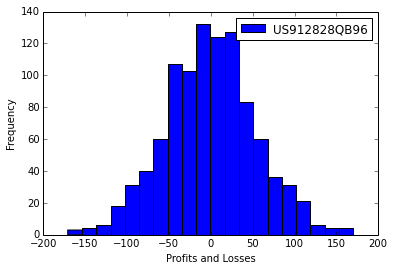
\includegraphics[max size={\textwidth}{\textheight}]{Market Risk Calculation_files/Market Risk Calculation_76_1.png}
    \par
    \end{center}
    
            \end{InvisibleVerbatim}
            
        
    


    % Make sure that atleast 4 lines are below the HR
    \needspace{4\baselineskip}

    
        \vspace{6pt}
        \makebox[0.1\linewidth]{\smaller\hfill\tt\color{nbframe-in-prompt}In\hspace{4pt}{[}36{]}:\hspace{4pt}}\\*
        \vspace{-2.65\baselineskip}
        \begin{ColorVerbatim}
            \vspace{-0.7\baselineskip}
            \begin{Verbatim}[commandchars=\\\{\}]
\PY{c}{\PYZsh{} Value\PYZhy{}at\PYZhy{}Risk for the Portfolio}
\PY{n}{plt}\PY{o}{.}\PY{n}{hist}\PY{p}{(}\PY{n}{port\PYZus{}pl}\PY{o}{.}\PY{n}{sum}\PY{p}{(}\PY{n}{axis}\PY{o}{=}\PY{l+m+mi}{1}\PY{p}{)}\PY{p}{,} \PY{l+m+mi}{20}\PY{p}{)}
\PY{n}{plt}\PY{o}{.}\PY{n}{ylabel}\PY{p}{(}\PY{l+s}{\PYZsq{}}\PY{l+s}{Frequency}\PY{l+s}{\PYZsq{}}\PY{p}{)}
\PY{n}{plt}\PY{o}{.}\PY{n}{xlabel}\PY{p}{(}\PY{l+s}{\PYZsq{}}\PY{l+s}{Profits and Losses}\PY{l+s}{\PYZsq{}}\PY{p}{)}
\PY{n}{plt}\PY{o}{.}\PY{n}{legend}\PY{p}{(}\PY{p}{[}\PY{l+s}{\PYZsq{}}\PY{l+s}{Portfolio}\PY{l+s}{\PYZsq{}}\PY{p}{]}\PY{p}{)}
\end{Verbatim}

            
                \vspace{-0.2\baselineskip}
            
        \end{ColorVerbatim}
    

    

        % If the first block is an image, minipage the image.  Else
        % request a certain amount of space for the input text.
        \needspace{4\baselineskip}
        
        

            % Add document contents.
            
                \makebox[0.1\linewidth]{\smaller\hfill\tt\color{nbframe-out-prompt}Out\hspace{4pt}{[}36{]}:\hspace{4pt}}\\*
                \vspace{-2.55\baselineskip}\begin{InvisibleVerbatim}
                \vspace{-0.5\baselineskip}
\begin{alltt}<matplotlib.legend.Legend at 0x11a672690>\end{alltt}

            \end{InvisibleVerbatim}
            
                \begin{InvisibleVerbatim}
                \vspace{-0.5\baselineskip}
    \begin{center}
    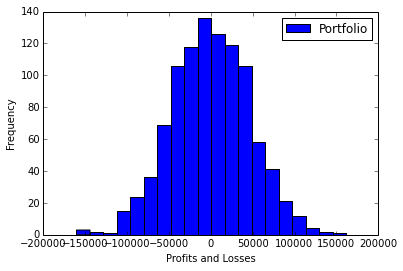
\includegraphics[max size={\textwidth}{\textheight}]{Market Risk Calculation_files/Market Risk Calculation_77_1.png}
    \par
    \end{center}
    
            \end{InvisibleVerbatim}
            
        
    
\part{Back testing}\section{For 2013}In order to measure the performance of this software, I did the
following analysis:

\begin{enumerate}
\def\labelenumi{\arabic{enumi}.}
\itemsep1pt\parskip0pt\parsep0pt
\item
  Created a Portfolio incluiding fixed-income securities and currency
  deposits according to the following table:
\end{enumerate}

Instrument type

Number of securities

weighting

US Treasury Bills

30

10.04

US Treasury Notes 1-5 years

150

38.65

US Treasury Notes 5-10 years

130

21.12

US Agencies 1-3 years

60

2.63

CA Govt. Notes 0-3 years

20

1.79

Euro (EUR)

1

11.54

Sterling Pound (GBP)

1

14.22

\begin{enumerate}
\def\labelenumi{\arabic{enumi}.}
\setcounter{enumi}{1}
\item
  Rebalancing the portfolio once each month
\item
  Calculate the daily market value for the portfolio and obtain the real
  profit and losses with observed market prices (full valuation, no
  factor-based valuation).
\item
  Calculate the daily Value at Risk for the aggregated portfolio and for
  each separated subportfolio specified in the table above.
\item
  Calculation from Jan 01, 2013 to Dec 31, 2013
\end{enumerate}\subsubsection{CAUTION!!! This code take several hours to be finished!!!}

    % Make sure that atleast 4 lines are below the HR
    \needspace{4\baselineskip}

    
        \vspace{6pt}
        \makebox[0.1\linewidth]{\smaller\hfill\tt\color{nbframe-in-prompt}In\hspace{4pt}{[}19{]}:\hspace{4pt}}\\*
        \vspace{-2.65\baselineskip}
        \begin{ColorVerbatim}
            \vspace{-0.7\baselineskip}
            \begin{Verbatim}[commandchars=\\\{\}]
\PY{n}{start} \PY{o}{=} \PY{n}{datetime}\PY{p}{(}\PY{l+m+mi}{2013}\PY{p}{,} \PY{l+m+mi}{12}\PY{p}{,} \PY{l+m+mi}{4}\PY{p}{)}
\PY{n}{end} \PY{o}{=} \PY{n}{datetime}\PY{p}{(}\PY{l+m+mi}{2013}\PY{p}{,} \PY{l+m+mi}{12}\PY{p}{,} \PY{l+m+mi}{31}\PY{p}{)}

\PY{n}{var\PYZus{}lever} \PY{o}{=} \PY{l+m+mi}{95}

\PY{n}{port\PYZus{}var\PYZus{}backtest} \PY{o}{=} \PY{p}{\PYZob{}}\PY{p}{\PYZcb{}}
\PY{n}{port\PYZus{}mtm\PYZus{}backtest} \PY{o}{=} \PY{p}{\PYZob{}}\PY{p}{\PYZcb{}}

\PY{k}{for} \PY{n}{calc\PYZus{}date} \PY{o+ow}{in} \PY{n}{pd}\PY{o}{.}\PY{n}{bdate\PYZus{}range}\PY{p}{(}\PY{n}{start}\PY{p}{,}\PY{n}{end}\PY{p}{)}\PY{p}{:}
    \PY{k}{if} \PY{n}{calc\PYZus{}date} \PY{o+ow}{in} \PY{n}{risk\PYZus{}factors\PYZus{}hist}\PY{o}{.}\PY{n}{index}\PY{p}{:}
        \PY{n}{port\PYZus{}file} \PY{o}{=} \PY{l+s}{\PYZsq{}}\PY{l+s}{port\PYZus{}}\PY{l+s}{\PYZsq{}} \PY{o}{+} \PY{n+nb}{str}\PY{p}{(}\PY{n}{calc\PYZus{}date}\PY{o}{.}\PY{n}{year}\PY{p}{)} \PY{o}{+} \PY{l+s}{\PYZsq{}}\PY{l+s}{\PYZhy{}}\PY{l+s}{\PYZsq{}} \PY{o}{+} \PY{n+nb}{str}\PY{p}{(}\PY{n}{calc\PYZus{}date}\PY{o}{.}\PY{n}{month}\PY{p}{)}\PY{o}{.}\PY{n}{zfill}\PY{p}{(}\PY{l+m+mi}{2}\PY{p}{)} \PY{o}{+} \PY{l+s}{\PYZsq{}}\PY{l+s}{.csv}\PY{l+s}{\PYZsq{}}
        \PY{n}{port} \PY{o}{=} \PY{n}{pd}\PY{o}{.}\PY{n}{read\PYZus{}csv}\PY{p}{(} \PY{n}{data\PYZus{}dir} \PY{o}{+} \PY{n}{port\PYZus{}file} \PY{p}{,} \PY{n}{na\PYZus{}values}\PY{o}{=}\PY{p}{[}\PY{l+s}{\PYZsq{}}\PY{l+s}{\PYZsq{}}\PY{p}{,}\PY{l+s}{\PYZsq{}}\PY{l+s}{NA}\PY{l+s}{\PYZsq{}}\PY{p}{,}\PY{l+s}{\PYZsq{}}\PY{l+s}{na}\PY{l+s}{\PYZsq{}}\PY{p}{,}\PY{l+s}{\PYZsq{}}\PY{l+s}{NaN}\PY{l+s}{\PYZsq{}}\PY{p}{,}\PY{l+s}{\PYZsq{}}\PY{l+s}{NULL}\PY{l+s}{\PYZsq{}}\PY{p}{]} \PY{p}{)}
        \PY{n}{port} \PY{o}{=} \PY{n}{pd}\PY{o}{.}\PY{n}{Series}\PY{p}{(}\PY{n}{port}\PY{o}{.}\PY{n}{position}\PY{o}{.}\PY{n}{values}\PY{p}{,}\PY{n}{index}\PY{o}{=}\PY{n}{port}\PY{o}{.}\PY{n}{id\PYZus{}instr}\PY{p}{)}
        
        \PY{k}{print} \PY{n}{calc\PYZus{}date}
        \PY{n}{risk\PYZus{}factors\PYZus{}sim} \PY{o}{=} \PY{n}{simulate\PYZus{}risk\PYZus{}factors}\PY{p}{(} \PY{n}{n\PYZus{}sim}\PY{o}{=}\PY{l+m+mi}{1000}\PY{p}{,}
                                                 \PY{n}{calc\PYZus{}date}\PY{o}{=}\PY{n}{calc\PYZus{}date}\PY{p}{,}
                                                 \PY{n}{risk\PYZus{}factors\PYZus{}hist}\PY{o}{=}\PY{n}{risk\PYZus{}factors\PYZus{}hist}\PY{p}{,}
                                                 \PY{n}{cur\PYZus{}flip}\PY{o}{=}\PY{n}{cur\PYZus{}flip}\PY{p}{,} \PY{n}{decay}\PY{o}{=}\PY{l+m+mf}{0.96}\PY{p}{,} \PY{n}{seed}\PY{o}{=}\PY{l+m+mi}{0} \PY{p}{)}
        \PY{n}{port\PYZus{}mtm\PYZus{}base} \PY{o}{=} \PY{n}{port\PYZus{}valuation}\PY{p}{(}\PY{n}{risk\PYZus{}factors}\PY{o}{=}\PY{n}{risk\PYZus{}factors\PYZus{}hist}\PY{o}{.}\PY{n}{ix}\PY{p}{[}\PY{n}{calc\PYZus{}date}\PY{p}{,}\PY{p}{]}\PY{p}{,}
                                       \PY{n}{port}\PY{o}{=}\PY{n}{port}\PY{p}{,}
                                       \PY{n}{instr\PYZus{}info}\PY{o}{=}\PY{n}{instr\PYZus{}info}\PY{p}{,}
                                       \PY{n}{cshf\PYZus{}info}\PY{o}{=}\PY{n}{cshf\PYZus{}info} \PY{p}{)}
        \PY{n}{port\PYZus{}mtm\PYZus{}sim} \PY{o}{=} \PY{n}{risk\PYZus{}factors\PYZus{}sim}\PY{o}{.}\PY{n}{apply}\PY{p}{(}\PY{n}{port\PYZus{}valuation}\PY{p}{,} \PY{n}{axis}\PY{o}{=}\PY{l+m+mi}{1}\PY{p}{,}
                                              \PY{n}{port}\PY{o}{=}\PY{n}{port}\PY{p}{,}
                                              \PY{n}{instr\PYZus{}info}\PY{o}{=}\PY{n}{instr\PYZus{}info}\PY{p}{,}
                                              \PY{n}{cshf\PYZus{}info}\PY{o}{=}\PY{n}{cshf\PYZus{}info} \PY{p}{)}
        \PY{n}{port\PYZus{}pl\PYZus{}sim} \PY{o}{=} \PY{n}{port\PYZus{}mtm\PYZus{}base} \PY{o}{\PYZhy{}} \PY{n}{port\PYZus{}mtm\PYZus{}sim}
        \PY{n}{port\PYZus{}mtm\PYZus{}backtest}\PY{p}{[}\PY{n}{calc\PYZus{}date}\PY{p}{]} \PY{o}{=} \PY{n}{port\PYZus{}mtm\PYZus{}base}\PY{o}{.}\PY{n}{sum}\PY{p}{(}\PY{p}{)}
        \PY{n}{port\PYZus{}var\PYZus{}backtest}\PY{p}{[}\PY{n}{calc\PYZus{}date}\PY{p}{]} \PY{o}{=} \PY{n}{np}\PY{o}{.}\PY{n}{percentile}\PY{p}{(} \PY{n}{port\PYZus{}pl\PYZus{}sim}\PY{o}{.}\PY{n}{sum}\PY{p}{(}\PY{n}{axis}\PY{o}{=}\PY{l+m+mi}{1}\PY{p}{)}\PY{p}{,} \PY{l+m+mi}{100}\PY{o}{\PYZhy{}}\PY{n}{var\PYZus{}lever} \PY{p}{)}
\end{Verbatim}

            
                \vspace{-0.2\baselineskip}
            
        \end{ColorVerbatim}
    

    

        % If the first block is an image, minipage the image.  Else
        % request a certain amount of space for the input text.
        \needspace{4\baselineskip}
        
        

            % Add document contents.
            
                \begin{InvisibleVerbatim}
                \vspace{-0.5\baselineskip}
\begin{alltt}2013-12-04 00:00:00
2013-12-05 00:00:00
2013-12-06 00:00:00
2013-12-09 00:00:00
2013-12-10 00:00:00
2013-12-11 00:00:00
2013-12-12 00:00:00
2013-12-13 00:00:00
2013-12-16 00:00:00
2013-12-17 00:00:00
2013-12-18 00:00:00
2013-12-19 00:00:00
2013-12-20 00:00:00
2013-12-23 00:00:00
2013-12-24 00:00:00
2013-12-26 00:00:00
2013-12-27 00:00:00
2013-12-30 00:00:00
2013-12-31 00:00:00
\end{alltt}

            \end{InvisibleVerbatim}
            
        
    


    % Make sure that atleast 4 lines are below the HR
    \needspace{4\baselineskip}

    
        \vspace{6pt}
        \makebox[0.1\linewidth]{\smaller\hfill\tt\color{nbframe-in-prompt}In\hspace{4pt}{[}29{]}:\hspace{4pt}}\\*
        \vspace{-2.65\baselineskip}
        \begin{ColorVerbatim}
            \vspace{-0.7\baselineskip}
            \begin{Verbatim}[commandchars=\\\{\}]
\PY{n}{port\PYZus{}mtm\PYZus{}backtest} \PY{o}{=} \PY{n}{pd}\PY{o}{.}\PY{n}{Series}\PY{p}{(}\PY{n}{port\PYZus{}mtm\PYZus{}backtest}\PY{p}{)}
\PY{n}{port\PYZus{}var\PYZus{}backtest} \PY{o}{=} \PY{n}{pd}\PY{o}{.}\PY{n}{Series}\PY{p}{(}\PY{n}{port\PYZus{}var\PYZus{}backtest}\PY{p}{)}

\PY{n}{port\PYZus{}mtm\PYZus{}backtest}\PY{o}{.}\PY{n}{to\PYZus{}csv}\PY{p}{(}\PY{n}{out\PYZus{}dir}\PY{o}{+}\PY{l+s}{\PYZsq{}}\PY{l+s}{backtesting\PYZus{}mtm.csv}\PY{l+s}{\PYZsq{}}\PY{p}{)}
\PY{n}{port\PYZus{}var\PYZus{}backtest}\PY{o}{.}\PY{n}{to\PYZus{}csv}\PY{p}{(}\PY{n}{out\PYZus{}dir}\PY{o}{+}\PY{l+s}{\PYZsq{}}\PY{l+s}{backtesting\PYZus{}var.csv}\PY{l+s}{\PYZsq{}}\PY{p}{)}
\end{Verbatim}

            
                \vspace{-0.2\baselineskip}
            
        \end{ColorVerbatim}
    


    % Make sure that atleast 4 lines are below the HR
    \needspace{4\baselineskip}

    
        \vspace{6pt}
        \makebox[0.1\linewidth]{\smaller\hfill\tt\color{nbframe-in-prompt}In\hspace{4pt}{[}38{]}:\hspace{4pt}}\\*
        \vspace{-2.65\baselineskip}
        \begin{ColorVerbatim}
            \vspace{-0.7\baselineskip}
            \begin{Verbatim}[commandchars=\\\{\}]
\PY{n}{port\PYZus{}mtm\PYZus{}backtest} \PY{o}{=} \PY{n}{pd}\PY{o}{.}\PY{n}{read\PYZus{}csv}\PY{p}{(} \PY{n}{out\PYZus{}dir}\PY{o}{+}\PY{l+s}{\PYZsq{}}\PY{l+s}{backtesting\PYZus{}mtm.csv}\PY{l+s}{\PYZsq{}} \PY{p}{,} \PY{n}{na\PYZus{}values}\PY{o}{=}\PY{p}{[}\PY{l+s}{\PYZsq{}}\PY{l+s}{\PYZsq{}}\PY{p}{,}\PY{l+s}{\PYZsq{}}\PY{l+s}{NA}\PY{l+s}{\PYZsq{}}\PY{p}{,}\PY{l+s}{\PYZsq{}}\PY{l+s}{na}\PY{l+s}{\PYZsq{}}\PY{p}{,}\PY{l+s}{\PYZsq{}}\PY{l+s}{NaN}\PY{l+s}{\PYZsq{}}\PY{p}{,}\PY{l+s}{\PYZsq{}}\PY{l+s}{NULL}\PY{l+s}{\PYZsq{}}\PY{p}{]} \PY{p}{,} \PY{n}{header}\PY{o}{=}\PY{l+m+mi}{0}\PY{p}{,} \PY{n}{names}\PY{o}{=}\PY{p}{[}\PY{l+s}{\PYZsq{}}\PY{l+s}{Date}\PY{l+s}{\PYZsq{}}\PY{p}{,}\PY{l+s}{\PYZsq{}}\PY{l+s}{mtm}\PY{l+s}{\PYZsq{}}\PY{p}{]}\PY{p}{)}
\PY{n}{port\PYZus{}var\PYZus{}backtest} \PY{o}{=} \PY{n}{pd}\PY{o}{.}\PY{n}{read\PYZus{}csv}\PY{p}{(} \PY{n}{out\PYZus{}dir}\PY{o}{+}\PY{l+s}{\PYZsq{}}\PY{l+s}{backtesting\PYZus{}var.csv}\PY{l+s}{\PYZsq{}} \PY{p}{,} \PY{n}{na\PYZus{}values}\PY{o}{=}\PY{p}{[}\PY{l+s}{\PYZsq{}}\PY{l+s}{\PYZsq{}}\PY{p}{,}\PY{l+s}{\PYZsq{}}\PY{l+s}{NA}\PY{l+s}{\PYZsq{}}\PY{p}{,}\PY{l+s}{\PYZsq{}}\PY{l+s}{na}\PY{l+s}{\PYZsq{}}\PY{p}{,}\PY{l+s}{\PYZsq{}}\PY{l+s}{NaN}\PY{l+s}{\PYZsq{}}\PY{p}{,}\PY{l+s}{\PYZsq{}}\PY{l+s}{NULL}\PY{l+s}{\PYZsq{}}\PY{p}{]} \PY{p}{,} \PY{n}{header}\PY{o}{=}\PY{l+m+mi}{0}\PY{p}{,} \PY{n}{names}\PY{o}{=}\PY{p}{[}\PY{l+s}{\PYZsq{}}\PY{l+s}{Date}\PY{l+s}{\PYZsq{}}\PY{p}{,}\PY{l+s}{\PYZsq{}}\PY{l+s}{var}\PY{l+s}{\PYZsq{}}\PY{p}{]}\PY{p}{)}

\PY{n}{port\PYZus{}mtm\PYZus{}backtest}\PY{p}{[}\PY{l+s}{\PYZsq{}}\PY{l+s}{Date}\PY{l+s}{\PYZsq{}}\PY{p}{]} \PY{o}{=} \PY{n}{pd}\PY{o}{.}\PY{n}{to\PYZus{}datetime}\PY{p}{(}\PY{n}{port\PYZus{}mtm\PYZus{}backtest}\PY{p}{[}\PY{l+s}{\PYZsq{}}\PY{l+s}{Date}\PY{l+s}{\PYZsq{}}\PY{p}{]}\PY{p}{)}
\PY{n}{port\PYZus{}var\PYZus{}backtest}\PY{p}{[}\PY{l+s}{\PYZsq{}}\PY{l+s}{Date}\PY{l+s}{\PYZsq{}}\PY{p}{]} \PY{o}{=} \PY{n}{pd}\PY{o}{.}\PY{n}{to\PYZus{}datetime}\PY{p}{(}\PY{n}{port\PYZus{}var\PYZus{}backtest}\PY{p}{[}\PY{l+s}{\PYZsq{}}\PY{l+s}{Date}\PY{l+s}{\PYZsq{}}\PY{p}{]}\PY{p}{)}

\PY{n}{port\PYZus{}mtm\PYZus{}backtest} \PY{o}{=} \PY{n}{port\PYZus{}mtm\PYZus{}backtest}\PY{o}{.}\PY{n}{set\PYZus{}index}\PY{p}{(}\PY{l+s}{\PYZsq{}}\PY{l+s}{Date}\PY{l+s}{\PYZsq{}}\PY{p}{)}\PY{p}{[}\PY{l+s}{\PYZsq{}}\PY{l+s}{mtm}\PY{l+s}{\PYZsq{}}\PY{p}{]}
\PY{n}{port\PYZus{}var\PYZus{}backtest} \PY{o}{=} \PY{n}{port\PYZus{}var\PYZus{}backtest}\PY{o}{.}\PY{n}{set\PYZus{}index}\PY{p}{(}\PY{l+s}{\PYZsq{}}\PY{l+s}{Date}\PY{l+s}{\PYZsq{}}\PY{p}{)}\PY{p}{[}\PY{l+s}{\PYZsq{}}\PY{l+s}{var}\PY{l+s}{\PYZsq{}}\PY{p}{]}

\PY{c}{\PYZsh{} Calculate observed profit and losses}
\PY{n}{port\PYZus{}pl\PYZus{}backtest} \PY{o}{=} \PY{n}{port\PYZus{}mtm\PYZus{}backtest} \PY{o}{\PYZhy{}} \PY{n}{port\PYZus{}mtm\PYZus{}backtest}\PY{o}{.}\PY{n}{shift}\PY{p}{(}\PY{l+m+mi}{1}\PY{p}{)}

\PY{c}{\PYZsh{} Eliminate profit and losses from first day in month}
\PY{c}{\PYZsh{} Rebalancing portfolio effect}

\PY{n}{port\PYZus{}pl\PYZus{}backtest} \PY{o}{=} \PY{n}{port\PYZus{}pl\PYZus{}backtest}\PY{o}{.}\PY{n}{drop}\PY{p}{(} \PY{n}{pd}\PY{o}{.}\PY{n}{to\PYZus{}datetime}\PY{p}{(} \PY{p}{[} \PY{l+s}{\PYZsq{}}\PY{l+s}{2013\PYZhy{}02\PYZhy{}01}\PY{l+s}{\PYZsq{}}\PY{p}{,} \PY{l+s}{\PYZsq{}}\PY{l+s}{2013\PYZhy{}03\PYZhy{}01}\PY{l+s}{\PYZsq{}}\PY{p}{,}
                                                           \PY{l+s}{\PYZsq{}}\PY{l+s}{2013\PYZhy{}04\PYZhy{}01}\PY{l+s}{\PYZsq{}}\PY{p}{,} \PY{l+s}{\PYZsq{}}\PY{l+s}{2013\PYZhy{}05\PYZhy{}01}\PY{l+s}{\PYZsq{}}\PY{p}{,} \PY{l+s}{\PYZsq{}}\PY{l+s}{2013\PYZhy{}06\PYZhy{}03}\PY{l+s}{\PYZsq{}}\PY{p}{,}
                                                           \PY{l+s}{\PYZsq{}}\PY{l+s}{2013\PYZhy{}07\PYZhy{}01}\PY{l+s}{\PYZsq{}}\PY{p}{,} \PY{l+s}{\PYZsq{}}\PY{l+s}{2013\PYZhy{}08\PYZhy{}01}\PY{l+s}{\PYZsq{}}\PY{p}{,} \PY{l+s}{\PYZsq{}}\PY{l+s}{2013\PYZhy{}09\PYZhy{}03}\PY{l+s}{\PYZsq{}}\PY{p}{,}
                                                           \PY{l+s}{\PYZsq{}}\PY{l+s}{2013\PYZhy{}10\PYZhy{}01}\PY{l+s}{\PYZsq{}}\PY{p}{,} \PY{l+s}{\PYZsq{}}\PY{l+s}{2013\PYZhy{}11\PYZhy{}01}\PY{l+s}{\PYZsq{}}\PY{p}{,} \PY{l+s}{\PYZsq{}}\PY{l+s}{2013\PYZhy{}12\PYZhy{}02}\PY{l+s}{\PYZsq{}}\PY{p}{]} \PY{p}{)} \PY{p}{)}
\PY{n}{port\PYZus{}pl\PYZus{}backtest} \PY{o}{=} \PY{n}{port\PYZus{}pl\PYZus{}backtest}\PY{o}{.}\PY{n}{dropna}\PY{p}{(}\PY{p}{)}
\PY{c}{\PYZsh{} print port\PYZus{}var\PYZus{}backtest}
\end{Verbatim}

            
                \vspace{-0.2\baselineskip}
            
        \end{ColorVerbatim}
    


    % Make sure that atleast 4 lines are below the HR
    \needspace{4\baselineskip}

    
        \vspace{6pt}
        \makebox[0.1\linewidth]{\smaller\hfill\tt\color{nbframe-in-prompt}In\hspace{4pt}{[}43{]}:\hspace{4pt}}\\*
        \vspace{-2.65\baselineskip}
        \begin{ColorVerbatim}
            \vspace{-0.7\baselineskip}
            \begin{Verbatim}[commandchars=\\\{\}]
\PY{n}{plt}\PY{o}{.}\PY{n}{plot}\PY{p}{(}\PY{n}{port\PYZus{}pl\PYZus{}backtest}\PY{o}{.}\PY{n}{index}\PY{p}{,} \PY{n}{port\PYZus{}pl\PYZus{}backtest}\PY{o}{.}\PY{n}{values}\PY{o}{/}\PY{l+m+mi}{1000}\PY{p}{,}
         \PY{n}{port\PYZus{}var\PYZus{}backtest}\PY{o}{.}\PY{n}{index}\PY{p}{,} \PY{n}{port\PYZus{}var\PYZus{}backtest}\PY{o}{.}\PY{n}{values}\PY{o}{/}\PY{l+m+mi}{1000} \PY{p}{)}
\PY{n}{plt}\PY{o}{.}\PY{n}{ylabel}\PY{p}{(}\PY{l+s}{\PYZsq{}}\PY{l+s}{Thousands of USD}\PY{l+s}{\PYZsq{}}\PY{p}{)}
\PY{n}{plt}\PY{o}{.}\PY{n}{xlabel}\PY{p}{(}\PY{l+s}{\PYZsq{}}\PY{l+s}{Date}\PY{l+s}{\PYZsq{}}\PY{p}{)}
\PY{n}{plt}\PY{o}{.}\PY{n}{legend}\PY{p}{(}\PY{p}{[}\PY{l+s}{\PYZsq{}}\PY{l+s}{profit and losses}\PY{l+s}{\PYZsq{}}\PY{p}{,}\PY{l+s}{\PYZsq{}}\PY{l+s}{Value at Risk}\PY{l+s}{\PYZsq{}}\PY{p}{]}\PY{p}{)}
\end{Verbatim}

            
                \vspace{-0.2\baselineskip}
            
        \end{ColorVerbatim}
    

    

        % If the first block is an image, minipage the image.  Else
        % request a certain amount of space for the input text.
        \needspace{4\baselineskip}
        
        

            % Add document contents.
            
                \makebox[0.1\linewidth]{\smaller\hfill\tt\color{nbframe-out-prompt}Out\hspace{4pt}{[}43{]}:\hspace{4pt}}\\*
                \vspace{-2.55\baselineskip}\begin{InvisibleVerbatim}
                \vspace{-0.5\baselineskip}
\begin{alltt}<matplotlib.legend.Legend at 0x11a86bc10>\end{alltt}

            \end{InvisibleVerbatim}
            
                \begin{InvisibleVerbatim}
                \vspace{-0.5\baselineskip}
    \begin{center}
    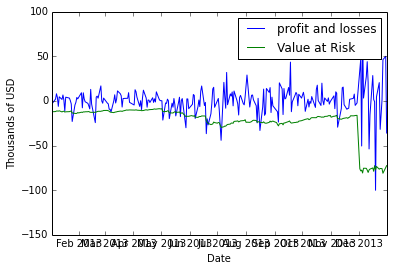
\includegraphics[max size={\textwidth}{\textheight}]{Market Risk Calculation_files/Market Risk Calculation_85_1.png}
    \par
    \end{center}
    
            \end{InvisibleVerbatim}
            
        
    
The results from this Backtesting exercise for evaluating the historical
performance of the 95\% confidence Value-at-Risk shows that only about
6\% of the observations fall below the estimated VaR.

This is a positive result, because it means that the metodology for
estimating the maximum loss in 95\% of the observed market scenarios is
being acurate.\part{Testing Suite}I realized that the fundamental parts in my code that are subject to
errors and have to be tested in order to ensure a proper output are the
following:

\begin{enumerate}
\def\labelenumi{\arabic{enumi}.}
\itemsep1pt\parskip0pt\parsep0pt
\item
  All the instruments defined in the portfolio are contained in the
  cashflows databases
\item
  Zero-coupon rates are being correctly calculated from yield to
  maturity values.
\item
  Valuation of a given instrument with a known set of rates is correct.
\end{enumerate}\section{Test 1: Portfolio cashflows are known}

    % Make sure that atleast 4 lines are below the HR
    \needspace{4\baselineskip}

    
        \vspace{6pt}
        \makebox[0.1\linewidth]{\smaller\hfill\tt\color{nbframe-in-prompt}In\hspace{4pt}{[}10{]}:\hspace{4pt}}\\*
        \vspace{-2.65\baselineskip}
        \begin{ColorVerbatim}
            \vspace{-0.7\baselineskip}
            \begin{Verbatim}[commandchars=\\\{\}]
\PY{o}{\PYZpc{}\PYZpc{}}\PY{k}{file} \PY{n}{test\PYZus{}01\PYZus{}instr\PYZus{}cshf}\PY{o}{.}\PY{n}{py}

\PY{k+kn}{import} \PY{n+nn}{numpy} \PY{k+kn}{as} \PY{n+nn}{np}
\PY{k+kn}{import} \PY{n+nn}{pandas} \PY{k+kn}{as} \PY{n+nn}{pd}
\PY{k+kn}{import} \PY{n+nn}{matplotlib.pyplot} \PY{k+kn}{as} \PY{n+nn}{plt}
\PY{k+kn}{import} \PY{n+nn}{urllib}
\PY{k+kn}{import} \PY{n+nn}{zipfile}

\PY{k+kn}{from} \PY{n+nn}{lxml} \PY{k+kn}{import} \PY{n}{etree}
\PY{k+kn}{from} \PY{n+nn}{scipy.interpolate} \PY{k+kn}{import} \PY{n}{interp1d}
\PY{k+kn}{from} \PY{n+nn}{datetime} \PY{k+kn}{import} \PY{n}{datetime}\PY{p}{,} \PY{n}{timedelta}
\PY{k+kn}{from} \PY{n+nn}{matplotlib.backends.backend\PYZus{}pdf} \PY{k+kn}{import} \PY{n}{PdfPages}

\PY{c}{\PYZsh{} Data directory \PYZsh{}}
\PY{n}{data\PYZus{}dir} \PY{o}{=} \PY{l+s}{\PYZsq{}}\PY{l+s}{/Users/Chris/Documents/26 UC Berkeley/03 Courses/STAT 222/stat\PYZus{}222\PYZus{}chris\PYZus{}carmona/data/}\PY{l+s}{\PYZsq{}}
\PY{n}{out\PYZus{}dir} \PY{o}{=} \PY{l+s}{\PYZsq{}}\PY{l+s}{/Users/Chris/Documents/26 UC Berkeley/03 Courses/STAT 222/stat\PYZus{}222\PYZus{}chris\PYZus{}carmona/output/}\PY{l+s}{\PYZsq{}}

\PY{c}{\PYZsh{} Portfolio file \PYZsh{}}
\PY{n}{port\PYZus{}file} \PY{o}{=} \PY{l+s}{\PYZsq{}}\PY{l+s}{port\PYZus{}2013\PYZhy{}12.csv}\PY{l+s}{\PYZsq{}}

\PY{c}{\PYZsh{} Portfolio \PYZsh{}}
\PY{n}{port} \PY{o}{=} \PY{n}{pd}\PY{o}{.}\PY{n}{read\PYZus{}csv}\PY{p}{(} \PY{n}{data\PYZus{}dir} \PY{o}{+} \PY{n}{port\PYZus{}file} \PY{p}{,} \PY{n}{na\PYZus{}values}\PY{o}{=}\PY{p}{[}\PY{l+s}{\PYZsq{}}\PY{l+s}{\PYZsq{}}\PY{p}{,}\PY{l+s}{\PYZsq{}}\PY{l+s}{NA}\PY{l+s}{\PYZsq{}}\PY{p}{,}\PY{l+s}{\PYZsq{}}\PY{l+s}{na}\PY{l+s}{\PYZsq{}}\PY{p}{,}\PY{l+s}{\PYZsq{}}\PY{l+s}{NaN}\PY{l+s}{\PYZsq{}}\PY{p}{,}\PY{l+s}{\PYZsq{}}\PY{l+s}{NULL}\PY{l+s}{\PYZsq{}}\PY{p}{]} \PY{p}{)}

\PY{n}{port} \PY{o}{=} \PY{n}{pd}\PY{o}{.}\PY{n}{Series}\PY{p}{(}\PY{n}{port}\PY{o}{.}\PY{n}{position}\PY{o}{.}\PY{n}{values}\PY{p}{,}\PY{n}{index}\PY{o}{=}\PY{n}{port}\PY{o}{.}\PY{n}{id\PYZus{}instr}\PY{p}{)}

\PY{c}{\PYZsh{} fixed\PYZhy{}income instruments cashflows \PYZsh{}}
\PY{n}{cshf\PYZus{}info\PYZus{}file} \PY{o}{=} \PY{l+s}{\PYZsq{}}\PY{l+s}{instr\PYZus{}cashflows.csv}\PY{l+s}{\PYZsq{}}
\PY{n}{cshf\PYZus{}info} \PY{o}{=} \PY{n}{pd}\PY{o}{.}\PY{n}{read\PYZus{}csv}\PY{p}{(} \PY{n}{data\PYZus{}dir} \PY{o}{+} \PY{n}{cshf\PYZus{}info\PYZus{}file} \PY{p}{,} \PY{n}{na\PYZus{}values}\PY{o}{=}\PY{p}{[}\PY{l+s}{\PYZsq{}}\PY{l+s}{\PYZsq{}}\PY{p}{,}\PY{l+s}{\PYZsq{}}\PY{l+s}{NA}\PY{l+s}{\PYZsq{}}\PY{p}{,}\PY{l+s}{\PYZsq{}}\PY{l+s}{na}\PY{l+s}{\PYZsq{}}\PY{p}{,}\PY{l+s}{\PYZsq{}}\PY{l+s}{NaN}\PY{l+s}{\PYZsq{}}\PY{p}{,}\PY{l+s}{\PYZsq{}}\PY{l+s}{NULL}\PY{l+s}{\PYZsq{}}\PY{p}{]} \PY{p}{)}
\PY{n}{cshf\PYZus{}info}\PY{p}{[}\PY{l+s}{\PYZsq{}}\PY{l+s}{Date}\PY{l+s}{\PYZsq{}}\PY{p}{]} \PY{o}{=} \PY{n}{pd}\PY{o}{.}\PY{n}{to\PYZus{}datetime}\PY{p}{(}\PY{n}{cshf\PYZus{}info}\PY{p}{[}\PY{l+s}{\PYZsq{}}\PY{l+s}{Date}\PY{l+s}{\PYZsq{}}\PY{p}{]}\PY{p}{)}
\PY{n}{cshf\PYZus{}info} \PY{o}{=} \PY{n}{cshf\PYZus{}info}\PY{o}{.}\PY{n}{groupby}\PY{p}{(}\PY{p}{[}\PY{l+s}{\PYZsq{}}\PY{l+s}{id\PYZus{}instr}\PY{l+s}{\PYZsq{}}\PY{p}{,}\PY{l+s}{\PYZsq{}}\PY{l+s}{Date}\PY{l+s}{\PYZsq{}}\PY{p}{]}\PY{p}{)}\PY{p}{[}\PY{l+s}{\PYZsq{}}\PY{l+s}{value}\PY{l+s}{\PYZsq{}}\PY{p}{]}\PY{o}{.}\PY{n}{sum}\PY{p}{(}\PY{p}{)}

\PY{k}{def} \PY{n+nf}{test\PYZus{}1}\PY{p}{(}\PY{p}{)}\PY{p}{:}

    \PY{n}{instr\PYZus{}name\PYZus{}len} \PY{o}{=} \PY{n}{np}\PY{o}{.}\PY{n}{array}\PY{p}{(} \PY{p}{[} \PY{n+nb}{len}\PY{p}{(}\PY{n}{i}\PY{p}{)} \PY{k}{for} \PY{n}{i} \PY{o+ow}{in}  \PY{n}{port}\PY{o}{.}\PY{n}{index}\PY{o}{.}\PY{n}{values} \PY{p}{]} \PY{p}{)}
    \PY{n}{instr\PYZus{}port} \PY{o}{=} \PY{n}{port}\PY{o}{.}\PY{n}{index}\PY{o}{.}\PY{n}{values}\PY{p}{[} \PY{n}{instr\PYZus{}name\PYZus{}len} \PY{o}{==} \PY{l+m+mi}{12} \PY{p}{]}
    
    \PY{n}{instr\PYZus{}port\PYZus{}defined} \PY{o}{=} \PY{p}{[} \PY{p}{(}\PY{n}{i} \PY{o+ow}{in} \PY{n}{cshf\PYZus{}info}\PY{o}{.}\PY{n}{unstack}\PY{p}{(}\PY{p}{)}\PY{o}{.}\PY{n}{index}\PY{o}{.}\PY{n}{values}\PY{p}{)} \PY{k}{for} \PY{n}{i} \PY{o+ow}{in} \PY{n}{instr\PYZus{}port} \PY{p}{]}
    
    \PY{n}{result} \PY{o}{=} \PY{n+nb}{all}\PY{p}{(}\PY{n}{instr\PYZus{}port\PYZus{}defined}\PY{p}{)} 
    \PY{k}{print} \PY{l+s}{\PYZsq{}}\PY{l+s}{Checking all instruments cashflows defined:}\PY{l+s}{\PYZsq{}}\PY{p}{,} \PY{n}{result}
    \PY{k}{assert} \PY{n}{result} \PY{o}{==} \PY{n+nb+bp}{True}

\PY{n}{test\PYZus{}1}\PY{p}{(}\PY{p}{)}
\end{Verbatim}

            
                \vspace{-0.2\baselineskip}
            
        \end{ColorVerbatim}
    

    

        % If the first block is an image, minipage the image.  Else
        % request a certain amount of space for the input text.
        \needspace{4\baselineskip}
        
        

            % Add document contents.
            
                \begin{InvisibleVerbatim}
                \vspace{-0.5\baselineskip}
\begin{alltt}Writing test\_01\_instr\_cshf.py
\end{alltt}

            \end{InvisibleVerbatim}
            
        
    
\section{Test 2: Zero-coupon calculation}

    % Make sure that atleast 4 lines are below the HR
    \needspace{4\baselineskip}

    
        \vspace{6pt}
        \makebox[0.1\linewidth]{\smaller\hfill\tt\color{nbframe-in-prompt}In\hspace{4pt}{[}11{]}:\hspace{4pt}}\\*
        \vspace{-2.65\baselineskip}
        \begin{ColorVerbatim}
            \vspace{-0.7\baselineskip}
            \begin{Verbatim}[commandchars=\\\{\}]
\PY{o}{\PYZpc{}\PYZpc{}}\PY{k}{file} \PY{n}{test\PYZus{}02\PYZus{}rates}\PY{o}{.}\PY{n}{py}

\PY{k+kn}{import} \PY{n+nn}{numpy} \PY{k+kn}{as} \PY{n+nn}{np}
\PY{k+kn}{import} \PY{n+nn}{pandas} \PY{k+kn}{as} \PY{n+nn}{pd}
\PY{k+kn}{import} \PY{n+nn}{matplotlib.pyplot} \PY{k+kn}{as} \PY{n+nn}{plt}
\PY{k+kn}{import} \PY{n+nn}{urllib}
\PY{k+kn}{import} \PY{n+nn}{zipfile}

\PY{k+kn}{from} \PY{n+nn}{lxml} \PY{k+kn}{import} \PY{n}{etree}
\PY{k+kn}{from} \PY{n+nn}{scipy.interpolate} \PY{k+kn}{import} \PY{n}{interp1d}
\PY{k+kn}{from} \PY{n+nn}{datetime} \PY{k+kn}{import} \PY{n}{datetime}\PY{p}{,} \PY{n}{timedelta}
\PY{k+kn}{from} \PY{n+nn}{matplotlib.backends.backend\PYZus{}pdf} \PY{k+kn}{import} \PY{n}{PdfPages}

\PY{c}{\PYZsh{} Data directory \PYZsh{}}
\PY{n}{data\PYZus{}dir} \PY{o}{=} \PY{l+s}{\PYZsq{}}\PY{l+s}{/Users/Chris/Documents/26 UC Berkeley/03 Courses/STAT 222/stat\PYZus{}222\PYZus{}chris\PYZus{}carmona/data/}\PY{l+s}{\PYZsq{}}
\PY{n}{out\PYZus{}dir} \PY{o}{=} \PY{l+s}{\PYZsq{}}\PY{l+s}{/Users/Chris/Documents/26 UC Berkeley/03 Courses/STAT 222/stat\PYZus{}222\PYZus{}chris\PYZus{}carmona/output/}\PY{l+s}{\PYZsq{}}

\PY{c}{\PYZsh{} Portfolio file \PYZsh{}}
\PY{n}{port\PYZus{}file} \PY{o}{=} \PY{l+s}{\PYZsq{}}\PY{l+s}{port\PYZus{}2013\PYZhy{}12.csv}\PY{l+s}{\PYZsq{}}

\PY{c}{\PYZsh{} Portfolio \PYZsh{}}
\PY{n}{port} \PY{o}{=} \PY{n}{pd}\PY{o}{.}\PY{n}{read\PYZus{}csv}\PY{p}{(} \PY{n}{data\PYZus{}dir} \PY{o}{+} \PY{n}{port\PYZus{}file} \PY{p}{,} \PY{n}{na\PYZus{}values}\PY{o}{=}\PY{p}{[}\PY{l+s}{\PYZsq{}}\PY{l+s}{\PYZsq{}}\PY{p}{,}\PY{l+s}{\PYZsq{}}\PY{l+s}{NA}\PY{l+s}{\PYZsq{}}\PY{p}{,}\PY{l+s}{\PYZsq{}}\PY{l+s}{na}\PY{l+s}{\PYZsq{}}\PY{p}{,}\PY{l+s}{\PYZsq{}}\PY{l+s}{NaN}\PY{l+s}{\PYZsq{}}\PY{p}{,}\PY{l+s}{\PYZsq{}}\PY{l+s}{NULL}\PY{l+s}{\PYZsq{}}\PY{p}{]} \PY{p}{)}

\PY{n}{port} \PY{o}{=} \PY{n}{pd}\PY{o}{.}\PY{n}{Series}\PY{p}{(}\PY{n}{port}\PY{o}{.}\PY{n}{position}\PY{o}{.}\PY{n}{values}\PY{p}{,}\PY{n}{index}\PY{o}{=}\PY{n}{port}\PY{o}{.}\PY{n}{id\PYZus{}instr}\PY{p}{)}

\PY{c}{\PYZsh{} fixed\PYZhy{}income instruments cashflows \PYZsh{}}
\PY{n}{cshf\PYZus{}info\PYZus{}file} \PY{o}{=} \PY{l+s}{\PYZsq{}}\PY{l+s}{instr\PYZus{}cashflows.csv}\PY{l+s}{\PYZsq{}}
\PY{n}{cshf\PYZus{}info} \PY{o}{=} \PY{n}{pd}\PY{o}{.}\PY{n}{read\PYZus{}csv}\PY{p}{(} \PY{n}{data\PYZus{}dir} \PY{o}{+} \PY{n}{cshf\PYZus{}info\PYZus{}file} \PY{p}{,} \PY{n}{na\PYZus{}values}\PY{o}{=}\PY{p}{[}\PY{l+s}{\PYZsq{}}\PY{l+s}{\PYZsq{}}\PY{p}{,}\PY{l+s}{\PYZsq{}}\PY{l+s}{NA}\PY{l+s}{\PYZsq{}}\PY{p}{,}\PY{l+s}{\PYZsq{}}\PY{l+s}{na}\PY{l+s}{\PYZsq{}}\PY{p}{,}\PY{l+s}{\PYZsq{}}\PY{l+s}{NaN}\PY{l+s}{\PYZsq{}}\PY{p}{,}\PY{l+s}{\PYZsq{}}\PY{l+s}{NULL}\PY{l+s}{\PYZsq{}}\PY{p}{]} \PY{p}{)}
\PY{n}{cshf\PYZus{}info}\PY{p}{[}\PY{l+s}{\PYZsq{}}\PY{l+s}{Date}\PY{l+s}{\PYZsq{}}\PY{p}{]} \PY{o}{=} \PY{n}{pd}\PY{o}{.}\PY{n}{to\PYZus{}datetime}\PY{p}{(}\PY{n}{cshf\PYZus{}info}\PY{p}{[}\PY{l+s}{\PYZsq{}}\PY{l+s}{Date}\PY{l+s}{\PYZsq{}}\PY{p}{]}\PY{p}{)}
\PY{n}{cshf\PYZus{}info} \PY{o}{=} \PY{n}{cshf\PYZus{}info}\PY{o}{.}\PY{n}{groupby}\PY{p}{(}\PY{p}{[}\PY{l+s}{\PYZsq{}}\PY{l+s}{id\PYZus{}instr}\PY{l+s}{\PYZsq{}}\PY{p}{,}\PY{l+s}{\PYZsq{}}\PY{l+s}{Date}\PY{l+s}{\PYZsq{}}\PY{p}{]}\PY{p}{)}\PY{p}{[}\PY{l+s}{\PYZsq{}}\PY{l+s}{value}\PY{l+s}{\PYZsq{}}\PY{p}{]}\PY{o}{.}\PY{n}{sum}\PY{p}{(}\PY{p}{)}

\PY{k}{def} \PY{n+nf}{zero\PYZus{}from\PYZus{}yield\PYZus{}bootstrap}\PY{p}{(} \PY{n}{ytm\PYZus{}curve} \PY{p}{,} \PY{n}{nodes} \PY{p}{)}\PY{p}{:}

    \PY{n}{nodes\PYZus{}old} \PY{o}{=} \PY{n}{nodes}\PY{o}{.}\PY{n}{copy}\PY{p}{(}\PY{p}{)}
    \PY{n}{nodes} \PY{o}{=} \PY{n}{np}\PY{o}{.}\PY{n}{append}\PY{p}{(}\PY{l+m+mi}{0}\PY{p}{,}\PY{n}{nodes}\PY{p}{)}
    \PY{n}{ytm\PYZus{}curve} \PY{o}{=} \PY{n}{np}\PY{o}{.}\PY{n}{append}\PY{p}{(}\PY{l+m+mi}{0}\PY{p}{,}\PY{n}{ytm\PYZus{}curve}\PY{p}{)}
    
    \PY{n}{nodes\PYZus{}new} \PY{o}{=} \PY{n}{np}\PY{o}{.}\PY{n}{arange}\PY{p}{(}\PY{l+m+mi}{0}\PY{p}{,}\PY{n+nb}{max}\PY{p}{(}\PY{n}{nodes}\PY{p}{)}\PY{o}{+}\PY{l+m+mf}{0.5}\PY{p}{,}\PY{l+m+mf}{0.5}\PY{p}{)}
    \PY{n}{nodes\PYZus{}new} \PY{o}{=} \PY{n}{np}\PY{o}{.}\PY{n}{append}\PY{p}{(}\PY{n}{nodes}\PY{p}{,}\PY{n}{nodes\PYZus{}new}\PY{p}{)}
    \PY{n}{nodes\PYZus{}new} \PY{o}{=} \PY{n}{np}\PY{o}{.}\PY{n}{sort}\PY{p}{(}\PY{n}{nodes\PYZus{}new}\PY{p}{)}
    \PY{n}{nodes\PYZus{}new} \PY{o}{=} \PY{n}{np}\PY{o}{.}\PY{n}{unique}\PY{p}{(}\PY{n}{nodes\PYZus{}new}\PY{p}{)}
        
    \PY{n}{f} \PY{o}{=} \PY{n}{interp1d}\PY{p}{(}\PY{n}{nodes}\PY{p}{,} \PY{n}{ytm\PYZus{}curve}\PY{p}{,} \PY{n}{kind}\PY{o}{=}\PY{l+s}{\PYZsq{}}\PY{l+s}{linear}\PY{l+s}{\PYZsq{}}\PY{p}{)}
    \PY{n}{ytm\PYZus{}new} \PY{o}{=} \PY{n}{f}\PY{p}{(}\PY{n}{nodes\PYZus{}new}\PY{p}{)}
    \PY{n}{ytm\PYZus{}new}\PY{p}{[}\PY{l+m+mi}{0}\PY{p}{]}\PY{o}{=}\PY{l+m+mi}{0}
    
    \PY{n}{ytm\PYZus{}new} \PY{o}{=} \PY{n}{pd}\PY{o}{.}\PY{n}{Series}\PY{p}{(}\PY{n}{ytm\PYZus{}new}\PY{p}{,}\PY{n}{index}\PY{o}{=}\PY{n}{nodes\PYZus{}new}\PY{p}{)}
    \PY{n}{zero\PYZus{}new} \PY{o}{=} \PY{n}{np}\PY{o}{.}\PY{n}{zeros\PYZus{}like}\PY{p}{(}\PY{n}{ytm\PYZus{}new}\PY{p}{)}
    
    \PY{n}{nodes\PYZus{}coupon} \PY{o}{=} \PY{n}{np}\PY{o}{.}\PY{n}{in1d}\PY{p}{(}\PY{n}{nodes\PYZus{}new}\PY{p}{,}\PY{n}{np}\PY{o}{.}\PY{n}{arange}\PY{p}{(}\PY{l+m+mi}{0}\PY{p}{,}\PY{n+nb}{max}\PY{p}{(}\PY{n}{nodes}\PY{p}{)}\PY{p}{,}\PY{l+m+mf}{0.5}\PY{p}{)}\PY{o}{+}\PY{l+m+mf}{0.5}\PY{p}{)}
    
    \PY{k}{for} \PY{n}{node\PYZus{}i} \PY{o+ow}{in} \PY{n}{nodes\PYZus{}new}\PY{p}{[}\PY{n}{nodes\PYZus{}coupon}\PY{o}{==}\PY{n+nb+bp}{False}\PY{p}{]}\PY{p}{:}
        \PY{n}{zero\PYZus{}new}\PY{p}{[}\PY{n}{node\PYZus{}i}\PY{p}{]} \PY{o}{=} \PY{p}{(}\PY{l+m+mi}{1}\PY{o}{+}\PY{n}{ytm\PYZus{}new}\PY{p}{[}\PY{n}{node\PYZus{}i}\PY{p}{]}\PY{o}{*}\PY{n}{node\PYZus{}i}\PY{p}{)} \PY{o}{*}\PY{o}{*} \PY{p}{(}\PY{l+m+mi}{1}\PY{o}{/}\PY{n}{node\PYZus{}i}\PY{p}{)}\PY{o}{\PYZhy{}}\PY{l+m+mi}{1}
    \PY{n}{zero\PYZus{}new}\PY{p}{[}\PY{l+m+mi}{0}\PY{p}{]} \PY{o}{=} \PY{l+m+mi}{0}
    
    
    \PY{k}{for} \PY{n}{node\PYZus{}i} \PY{o+ow}{in} \PY{n}{nodes\PYZus{}new}\PY{p}{[}\PY{n}{nodes\PYZus{}coupon}\PY{p}{]}\PY{p}{:}
        \PY{n}{cpn\PYZus{}i} \PY{o}{=} \PY{n}{ytm\PYZus{}new}\PY{p}{[}\PY{n}{node\PYZus{}i}\PY{p}{]}\PY{o}{/}\PY{l+m+mi}{2}
        \PY{n}{zero\PYZus{}new}\PY{p}{[}\PY{n}{node\PYZus{}i}\PY{p}{]} \PY{o}{=} \PY{o}{\PYZhy{}} \PY{n}{np}\PY{o}{.}\PY{n}{log}\PY{p}{(} \PY{p}{(}\PY{l+m+mi}{1} \PY{o}{\PYZhy{}} \PY{n}{cpn\PYZus{}i} \PY{o}{*} \PY{n}{np}\PY{o}{.}\PY{n}{exp}\PY{p}{(}\PY{o}{\PYZhy{}}\PY{n}{nodes\PYZus{}new}\PY{p}{[} \PY{n}{nodes\PYZus{}new}\PY{o}{\PYZlt{}}\PY{n}{node\PYZus{}i} \PY{o}{*} \PY{n}{nodes\PYZus{}coupon} \PY{p}{]} \PY{o}{*} \PY{n}{zero\PYZus{}new}\PY{p}{[} \PY{n}{nodes\PYZus{}new}\PY{o}{\PYZlt{}}\PY{n}{node\PYZus{}i} \PY{o}{*} \PY{n}{nodes\PYZus{}coupon} \PY{p}{]}\PY{p}{)}\PY{o}{.}\PY{n}{sum}\PY{p}{(}\PY{p}{)}\PY{p}{)}\PY{o}{/}\PY{p}{(}\PY{l+m+mi}{1}\PY{o}{+}\PY{n}{cpn\PYZus{}i}\PY{p}{)} \PY{p}{)} \PY{o}{*} \PY{p}{(}\PY{l+m+mi}{1}\PY{o}{/}\PY{n}{node\PYZus{}i}\PY{p}{)}

        
    \PY{k}{return} \PY{n}{zero\PYZus{}new}\PY{p}{[}\PY{n}{np}\PY{o}{.}\PY{n}{in1d}\PY{p}{(}\PY{n}{nodes\PYZus{}new}\PY{p}{,}\PY{n}{nodes\PYZus{}old}\PY{p}{)}\PY{p}{]}\PY{o}{.}\PY{n}{values}

\PY{k}{def} \PY{n+nf}{test\PYZus{}2}\PY{p}{(}\PY{p}{)}\PY{p}{:}
    \PY{n}{nodes} \PY{o}{=} \PY{n}{np}\PY{o}{.}\PY{n}{array}\PY{p}{(}\PY{n+nb}{range}\PY{p}{(}\PY{l+m+mi}{1}\PY{p}{,}\PY{l+m+mi}{31}\PY{p}{)}\PY{p}{,}\PY{n}{dtype}\PY{o}{=}\PY{n}{np}\PY{o}{.}\PY{n}{float64}\PY{p}{)}
    \PY{n}{ytm\PYZus{}curve\PYZus{}test} \PY{o}{=} \PY{n}{pd}\PY{o}{.}\PY{n}{Series}\PY{p}{(} \PY{n}{np}\PY{o}{.}\PY{n}{zeros\PYZus{}like}\PY{p}{(}\PY{n}{nodes}\PY{p}{)}\PY{o}{+}\PY{l+m+mf}{0.05} \PY{p}{,} \PY{n}{index}\PY{o}{=}\PY{n}{nodes}\PY{p}{)}
    \PY{n}{zero\PYZus{}curve\PYZus{}test} \PY{o}{=} \PY{n}{zero\PYZus{}from\PYZus{}yield\PYZus{}bootstrap}\PY{p}{(} \PY{n}{ytm\PYZus{}curve}\PY{o}{=}\PY{n}{ytm\PYZus{}curve\PYZus{}test}\PY{o}{.}\PY{n}{values} \PY{p}{,} \PY{n}{nodes}\PY{o}{=}\PY{n}{nodes} \PY{p}{)}
    \PY{n}{zero\PYZus{}curve\PYZus{}test} \PY{o}{=} \PY{n}{np}\PY{o}{.}\PY{n}{array}\PY{p}{(} \PY{p}{[} \PY{n+nb}{round}\PY{p}{(}\PY{n}{rate}\PY{p}{,} \PY{l+m+mi}{2}\PY{p}{)} \PY{k}{for} \PY{n}{rate} \PY{o+ow}{in} \PY{n}{zero\PYZus{}curve\PYZus{}test} \PY{p}{]}\PY{p}{,}\PY{n}{dtype}\PY{o}{=}\PY{n}{np}\PY{o}{.}\PY{n}{float64}\PY{p}{)}
    \PY{n}{result} \PY{o}{=} \PY{n+nb}{all}\PY{p}{(} \PY{n}{ytm\PYZus{}curve\PYZus{}test} \PY{o}{==} \PY{n}{zero\PYZus{}curve\PYZus{}test} \PY{p}{)}
    
    \PY{k}{print} \PY{l+s}{\PYZsq{}}\PY{l+s}{Checking zero rates:}\PY{l+s}{\PYZsq{}}\PY{p}{,} \PY{n}{result}
    \PY{k}{assert} \PY{n}{result} \PY{o}{==} \PY{n+nb+bp}{True}

\PY{n}{test\PYZus{}2}\PY{p}{(}\PY{p}{)}
\end{Verbatim}

            
                \vspace{-0.2\baselineskip}
            
        \end{ColorVerbatim}
    

    

        % If the first block is an image, minipage the image.  Else
        % request a certain amount of space for the input text.
        \needspace{4\baselineskip}
        
        

            % Add document contents.
            
                \begin{InvisibleVerbatim}
                \vspace{-0.5\baselineskip}
\begin{alltt}Writing test\_02\_rates.py
\end{alltt}

            \end{InvisibleVerbatim}
            
        
    
\section{Test 3-4: Instrument valuation}

    % Make sure that atleast 4 lines are below the HR
    \needspace{4\baselineskip}

    
        \vspace{6pt}
        \makebox[0.1\linewidth]{\smaller\hfill\tt\color{nbframe-in-prompt}In\hspace{4pt}{[}12{]}:\hspace{4pt}}\\*
        \vspace{-2.65\baselineskip}
        \begin{ColorVerbatim}
            \vspace{-0.7\baselineskip}
            \begin{Verbatim}[commandchars=\\\{\}]
\PY{o}{\PYZpc{}\PYZpc{}}\PY{k}{file} \PY{n}{test\PYZus{}03\PYZus{}valuation}\PY{o}{.}\PY{n}{py}

\PY{k+kn}{import} \PY{n+nn}{numpy} \PY{k+kn}{as} \PY{n+nn}{np}
\PY{k+kn}{import} \PY{n+nn}{pandas} \PY{k+kn}{as} \PY{n+nn}{pd}
\PY{k+kn}{import} \PY{n+nn}{matplotlib.pyplot} \PY{k+kn}{as} \PY{n+nn}{plt}
\PY{k+kn}{import} \PY{n+nn}{urllib}
\PY{k+kn}{import} \PY{n+nn}{zipfile}

\PY{k+kn}{from} \PY{n+nn}{lxml} \PY{k+kn}{import} \PY{n}{etree}
\PY{k+kn}{from} \PY{n+nn}{scipy.interpolate} \PY{k+kn}{import} \PY{n}{interp1d}
\PY{k+kn}{from} \PY{n+nn}{datetime} \PY{k+kn}{import} \PY{n}{datetime}\PY{p}{,} \PY{n}{timedelta}
\PY{k+kn}{from} \PY{n+nn}{matplotlib.backends.backend\PYZus{}pdf} \PY{k+kn}{import} \PY{n}{PdfPages}

\PY{c}{\PYZsh{} Data directory \PYZsh{}}
\PY{n}{data\PYZus{}dir} \PY{o}{=} \PY{l+s}{\PYZsq{}}\PY{l+s}{/Users/Chris/Documents/26 UC Berkeley/03 Courses/STAT 222/stat\PYZus{}222\PYZus{}chris\PYZus{}carmona/data/}\PY{l+s}{\PYZsq{}}
\PY{n}{out\PYZus{}dir} \PY{o}{=} \PY{l+s}{\PYZsq{}}\PY{l+s}{/Users/Chris/Documents/26 UC Berkeley/03 Courses/STAT 222/stat\PYZus{}222\PYZus{}chris\PYZus{}carmona/output/}\PY{l+s}{\PYZsq{}}

\PY{c}{\PYZsh{} Portfolio file \PYZsh{}}
\PY{n}{port\PYZus{}file} \PY{o}{=} \PY{l+s}{\PYZsq{}}\PY{l+s}{port\PYZus{}2013\PYZhy{}12.csv}\PY{l+s}{\PYZsq{}}

\PY{c}{\PYZsh{} Portfolio \PYZsh{}}
\PY{n}{port} \PY{o}{=} \PY{n}{pd}\PY{o}{.}\PY{n}{read\PYZus{}csv}\PY{p}{(} \PY{n}{data\PYZus{}dir} \PY{o}{+} \PY{n}{port\PYZus{}file} \PY{p}{,} \PY{n}{na\PYZus{}values}\PY{o}{=}\PY{p}{[}\PY{l+s}{\PYZsq{}}\PY{l+s}{\PYZsq{}}\PY{p}{,}\PY{l+s}{\PYZsq{}}\PY{l+s}{NA}\PY{l+s}{\PYZsq{}}\PY{p}{,}\PY{l+s}{\PYZsq{}}\PY{l+s}{na}\PY{l+s}{\PYZsq{}}\PY{p}{,}\PY{l+s}{\PYZsq{}}\PY{l+s}{NaN}\PY{l+s}{\PYZsq{}}\PY{p}{,}\PY{l+s}{\PYZsq{}}\PY{l+s}{NULL}\PY{l+s}{\PYZsq{}}\PY{p}{]} \PY{p}{)}

\PY{n}{port} \PY{o}{=} \PY{n}{pd}\PY{o}{.}\PY{n}{Series}\PY{p}{(}\PY{n}{port}\PY{o}{.}\PY{n}{position}\PY{o}{.}\PY{n}{values}\PY{p}{,}\PY{n}{index}\PY{o}{=}\PY{n}{port}\PY{o}{.}\PY{n}{id\PYZus{}instr}\PY{p}{)}

\PY{c}{\PYZsh{} fixed\PYZhy{}income instruments cashflows \PYZsh{}}
\PY{n}{cshf\PYZus{}info\PYZus{}file} \PY{o}{=} \PY{l+s}{\PYZsq{}}\PY{l+s}{instr\PYZus{}cashflows.csv}\PY{l+s}{\PYZsq{}}
\PY{n}{cshf\PYZus{}info} \PY{o}{=} \PY{n}{pd}\PY{o}{.}\PY{n}{read\PYZus{}csv}\PY{p}{(} \PY{n}{data\PYZus{}dir} \PY{o}{+} \PY{n}{cshf\PYZus{}info\PYZus{}file} \PY{p}{,} \PY{n}{na\PYZus{}values}\PY{o}{=}\PY{p}{[}\PY{l+s}{\PYZsq{}}\PY{l+s}{\PYZsq{}}\PY{p}{,}\PY{l+s}{\PYZsq{}}\PY{l+s}{NA}\PY{l+s}{\PYZsq{}}\PY{p}{,}\PY{l+s}{\PYZsq{}}\PY{l+s}{na}\PY{l+s}{\PYZsq{}}\PY{p}{,}\PY{l+s}{\PYZsq{}}\PY{l+s}{NaN}\PY{l+s}{\PYZsq{}}\PY{p}{,}\PY{l+s}{\PYZsq{}}\PY{l+s}{NULL}\PY{l+s}{\PYZsq{}}\PY{p}{]} \PY{p}{)}
\PY{n}{cshf\PYZus{}info}\PY{p}{[}\PY{l+s}{\PYZsq{}}\PY{l+s}{Date}\PY{l+s}{\PYZsq{}}\PY{p}{]} \PY{o}{=} \PY{n}{pd}\PY{o}{.}\PY{n}{to\PYZus{}datetime}\PY{p}{(}\PY{n}{cshf\PYZus{}info}\PY{p}{[}\PY{l+s}{\PYZsq{}}\PY{l+s}{Date}\PY{l+s}{\PYZsq{}}\PY{p}{]}\PY{p}{)}
\PY{n}{cshf\PYZus{}info} \PY{o}{=} \PY{n}{cshf\PYZus{}info}\PY{o}{.}\PY{n}{groupby}\PY{p}{(}\PY{p}{[}\PY{l+s}{\PYZsq{}}\PY{l+s}{id\PYZus{}instr}\PY{l+s}{\PYZsq{}}\PY{p}{,}\PY{l+s}{\PYZsq{}}\PY{l+s}{Date}\PY{l+s}{\PYZsq{}}\PY{p}{]}\PY{p}{)}\PY{p}{[}\PY{l+s}{\PYZsq{}}\PY{l+s}{value}\PY{l+s}{\PYZsq{}}\PY{p}{]}\PY{o}{.}\PY{n}{sum}\PY{p}{(}\PY{p}{)}

\PY{c}{\PYZsh{} instruments description \PYZsh{}}
\PY{n}{instr\PYZus{}info\PYZus{}file} \PY{o}{=} \PY{l+s}{\PYZsq{}}\PY{l+s}{instr\PYZus{}description.csv}\PY{l+s}{\PYZsq{}}
\PY{n}{instr\PYZus{}info} \PY{o}{=} \PY{n}{pd}\PY{o}{.}\PY{n}{read\PYZus{}csv}\PY{p}{(} \PY{n}{data\PYZus{}dir} \PY{o}{+} \PY{n}{instr\PYZus{}info\PYZus{}file} \PY{p}{,} \PY{n}{na\PYZus{}values}\PY{o}{=}\PY{p}{[}\PY{l+s}{\PYZsq{}}\PY{l+s}{\PYZsq{}}\PY{p}{,}\PY{l+s}{\PYZsq{}}\PY{l+s}{NA}\PY{l+s}{\PYZsq{}}\PY{p}{,}\PY{l+s}{\PYZsq{}}\PY{l+s}{na}\PY{l+s}{\PYZsq{}}\PY{p}{,}\PY{l+s}{\PYZsq{}}\PY{l+s}{NaN}\PY{l+s}{\PYZsq{}}\PY{p}{,}\PY{l+s}{\PYZsq{}}\PY{l+s}{NULL}\PY{l+s}{\PYZsq{}}\PY{p}{]} \PY{p}{)}

\PY{n}{currencies} \PY{o}{=} \PY{p}{[}\PY{l+s}{\PYZsq{}}\PY{l+s}{AUD}\PY{l+s}{\PYZsq{}}\PY{p}{,} \PY{l+s}{\PYZsq{}}\PY{l+s}{CAD}\PY{l+s}{\PYZsq{}}\PY{p}{,} \PY{l+s}{\PYZsq{}}\PY{l+s}{CHF}\PY{l+s}{\PYZsq{}}\PY{p}{,} \PY{l+s}{\PYZsq{}}\PY{l+s}{CLP}\PY{l+s}{\PYZsq{}}\PY{p}{,} \PY{l+s}{\PYZsq{}}\PY{l+s}{EUR}\PY{l+s}{\PYZsq{}}\PY{p}{,} \PY{l+s}{\PYZsq{}}\PY{l+s}{GBP}\PY{l+s}{\PYZsq{}}\PY{p}{,} \PY{l+s}{\PYZsq{}}\PY{l+s}{JPY}\PY{l+s}{\PYZsq{}}\PY{p}{,} \PY{l+s}{\PYZsq{}}\PY{l+s}{NOK}\PY{l+s}{\PYZsq{}}\PY{p}{,} \PY{l+s}{\PYZsq{}}\PY{l+s}{NZD}\PY{l+s}{\PYZsq{}}\PY{p}{,} \PY{l+s}{\PYZsq{}}\PY{l+s}{SEK}\PY{l+s}{\PYZsq{}}\PY{p}{,} \PY{l+s}{\PYZsq{}}\PY{l+s}{SGD}\PY{l+s}{\PYZsq{}}\PY{p}{]}
\PY{c}{\PYZsh{} Flip all currencies to dollars per curency}
\PY{n}{cur\PYZus{}usd} \PY{o}{=} \PY{p}{[}\PY{l+s}{\PYZsq{}}\PY{l+s}{AUD}\PY{l+s}{\PYZsq{}}\PY{p}{,} \PY{l+s}{\PYZsq{}}\PY{l+s}{EUR}\PY{l+s}{\PYZsq{}}\PY{p}{,} \PY{l+s}{\PYZsq{}}\PY{l+s}{GBP}\PY{l+s}{\PYZsq{}}\PY{p}{,} \PY{l+s}{\PYZsq{}}\PY{l+s}{NZD}\PY{l+s}{\PYZsq{}}\PY{p}{]}
\PY{n}{cur\PYZus{}flip} \PY{o}{=} \PY{n+nb}{list}\PY{p}{(}\PY{n+nb}{set}\PY{p}{(}\PY{n}{currencies}\PY{p}{)}\PY{o}{.}\PY{n}{difference}\PY{p}{(}\PY{n+nb}{set}\PY{p}{(}\PY{n}{cur\PYZus{}usd}\PY{p}{)}\PY{p}{)}\PY{p}{)}


\PY{n}{nodes} \PY{o}{=} \PY{n}{np}\PY{o}{.}\PY{n}{array}\PY{p}{(}\PY{p}{[}\PY{l+m+mi}{1}\PY{p}{,}\PY{l+m+mi}{3}\PY{p}{,}\PY{l+m+mi}{6}\PY{p}{]}\PY{p}{,}\PY{n}{dtype}\PY{o}{=}\PY{n}{np}\PY{o}{.}\PY{n}{float64}\PY{p}{)}
\PY{n}{nodes} \PY{o}{=} \PY{n}{nodes}\PY{o}{/}\PY{l+m+mi}{12}
\PY{n}{nodes} \PY{o}{=} \PY{n}{np}\PY{o}{.}\PY{n}{append}\PY{p}{(}\PY{n}{nodes}\PY{p}{,} \PY{n}{np}\PY{o}{.}\PY{n}{array}\PY{p}{(}\PY{p}{[}\PY{l+m+mi}{1}\PY{p}{,}\PY{l+m+mi}{2}\PY{p}{,}\PY{l+m+mi}{3}\PY{p}{,}\PY{l+m+mi}{5}\PY{p}{,}\PY{l+m+mi}{7}\PY{p}{,}\PY{l+m+mi}{10}\PY{p}{,}\PY{l+m+mi}{20}\PY{p}{,}\PY{l+m+mi}{30}\PY{p}{]}\PY{p}{,}\PY{n}{dtype}\PY{o}{=}\PY{n}{np}\PY{o}{.}\PY{n}{float64}\PY{p}{)} \PY{p}{)}
\PY{n}{nodes\PYZus{}names} \PY{o}{=} \PY{p}{[}\PY{l+s}{\PYZsq{}}\PY{l+s}{GOVT\PYZus{}USD\PYZus{}USA\PYZus{}1m}\PY{l+s}{\PYZsq{}}\PY{p}{,}\PY{l+s}{\PYZsq{}}\PY{l+s}{GOVT\PYZus{}USD\PYZus{}USA\PYZus{}3m}\PY{l+s}{\PYZsq{}}\PY{p}{,}\PY{l+s}{\PYZsq{}}\PY{l+s}{GOVT\PYZus{}USD\PYZus{}USA\PYZus{}6m}\PY{l+s}{\PYZsq{}}\PY{p}{,}
               \PY{l+s}{\PYZsq{}}\PY{l+s}{GOVT\PYZus{}USD\PYZus{}USA\PYZus{}1y}\PY{l+s}{\PYZsq{}}\PY{p}{,}\PY{l+s}{\PYZsq{}}\PY{l+s}{GOVT\PYZus{}USD\PYZus{}USA\PYZus{}2y}\PY{l+s}{\PYZsq{}}\PY{p}{,}\PY{l+s}{\PYZsq{}}\PY{l+s}{GOVT\PYZus{}USD\PYZus{}USA\PYZus{}3y}\PY{l+s}{\PYZsq{}}\PY{p}{,}
               \PY{l+s}{\PYZsq{}}\PY{l+s}{GOVT\PYZus{}USD\PYZus{}USA\PYZus{}5y}\PY{l+s}{\PYZsq{}}\PY{p}{,}\PY{l+s}{\PYZsq{}}\PY{l+s}{GOVT\PYZus{}USD\PYZus{}USA\PYZus{}7y}\PY{l+s}{\PYZsq{}}\PY{p}{,}\PY{l+s}{\PYZsq{}}\PY{l+s}{GOVT\PYZus{}USD\PYZus{}USA\PYZus{}10y}\PY{l+s}{\PYZsq{}}\PY{p}{,}
               \PY{l+s}{\PYZsq{}}\PY{l+s}{GOVT\PYZus{}USD\PYZus{}USA\PYZus{}20y}\PY{l+s}{\PYZsq{}}\PY{p}{,}\PY{l+s}{\PYZsq{}}\PY{l+s}{GOVT\PYZus{}USD\PYZus{}USA\PYZus{}30y}\PY{l+s}{\PYZsq{}}\PY{p}{]}

\PY{k}{def} \PY{n+nf}{port\PYZus{}valuation}\PY{p}{(} \PY{n}{port}\PY{p}{,} \PY{n}{calc\PYZus{}date}\PY{p}{,} \PY{n}{risk\PYZus{}factors}\PY{p}{,} \PY{n}{instr\PYZus{}info}\PY{p}{,} \PY{n}{cshf\PYZus{}info}\PY{p}{)}\PY{p}{:}
    \PY{c}{\PYZsh{} Cash flows for bonds}
    \PY{n}{bonds\PYZus{}cshf} \PY{o}{=} \PY{n}{cshf\PYZus{}info}\PY{o}{.}\PY{n}{ix}\PY{p}{[} \PY{n}{port}\PY{o}{.}\PY{n}{index}\PY{o}{.}\PY{n}{values} \PY{p}{]}\PY{o}{.}\PY{n}{unstack}\PY{p}{(}\PY{l+s}{\PYZsq{}}\PY{l+s}{id\PYZus{}instr}\PY{l+s}{\PYZsq{}}\PY{p}{)}
    \PY{n}{bonds\PYZus{}cshf} \PY{o}{=} \PY{n}{bonds\PYZus{}cshf}\PY{p}{[}\PY{n}{bonds\PYZus{}cshf}\PY{o}{.}\PY{n}{index}\PY{o}{\PYZgt{}}\PY{o}{=}\PY{n}{calc\PYZus{}date}\PY{p}{]}
    \PY{n}{bonds\PYZus{}cshf} \PY{o}{=} \PY{n}{bonds\PYZus{}cshf}\PY{o}{/}\PY{l+m+mi}{1000000}
    \PY{n}{bonds\PYZus{}cshf} \PY{o}{=} \PY{n}{bonds\PYZus{}cshf} \PY{o}{*} \PY{n}{port}\PY{p}{[}\PY{n}{bonds\PYZus{}cshf}\PY{o}{.}\PY{n}{columns}\PY{p}{]}
    
    \PY{c}{\PYZsh{} Cash flows for currencies}
    \PY{n}{ccy\PYZus{}cshf} \PY{o}{=} \PY{n}{port}\PY{p}{[}\PY{n}{currencies}\PY{p}{]}\PY{o}{.}\PY{n}{dropna}\PY{p}{(}\PY{p}{)}
    \PY{n}{ccy\PYZus{}cshf} \PY{o}{=} \PY{n}{pd}\PY{o}{.}\PY{n}{DataFrame}\PY{p}{(} \PY{n}{ccy\PYZus{}cshf}\PY{o}{.}\PY{n}{values}\PY{p}{,} \PY{n}{index}\PY{o}{=}\PY{n}{ccy\PYZus{}cshf}\PY{o}{.}\PY{n}{index}\PY{p}{,} \PY{n}{columns}\PY{o}{=}\PY{p}{[}\PY{n}{calc\PYZus{}date}\PY{p}{]} \PY{p}{)}\PY{o}{.}\PY{n}{T}
    \PY{k}{if} \PY{l+s}{\PYZsq{}}\PY{l+s}{USD}\PY{l+s}{\PYZsq{}} \PY{o+ow}{in} \PY{n}{port}\PY{o}{.}\PY{n}{index}\PY{p}{:}
        \PY{n}{ccy\PYZus{}cshf}\PY{p}{[}\PY{l+s}{\PYZsq{}}\PY{l+s}{USD}\PY{l+s}{\PYZsq{}}\PY{p}{]} \PY{o}{=} \PY{n}{port}\PY{p}{[}\PY{l+s}{\PYZsq{}}\PY{l+s}{USD}\PY{l+s}{\PYZsq{}}\PY{p}{]}
    
    \PY{c}{\PYZsh{} cashflows for all the portfolio}
    \PY{n}{port\PYZus{}cshf} \PY{o}{=} \PY{n}{pd}\PY{o}{.}\PY{n}{merge}\PY{p}{(} \PY{n}{ccy\PYZus{}cshf}\PY{p}{,} \PY{n}{bonds\PYZus{}cshf}\PY{p}{,} \PY{n}{left\PYZus{}index}\PY{o}{=}\PY{n+nb+bp}{True}\PY{p}{,} \PY{n}{right\PYZus{}index}\PY{o}{=}\PY{n+nb+bp}{True}\PY{p}{,} \PY{n}{how}\PY{o}{=}\PY{l+s}{\PYZsq{}}\PY{l+s}{outer}\PY{l+s}{\PYZsq{}} \PY{p}{)}
    \PY{n}{port\PYZus{}cshf}\PY{o}{.}\PY{n}{dropna}\PY{p}{(} \PY{n}{how}\PY{o}{=}\PY{l+s}{\PYZsq{}}\PY{l+s}{all}\PY{l+s}{\PYZsq{}} \PY{p}{)}
    
    \PY{c}{\PYZsh{} Discount factors calculation}
    \PY{n}{discount} \PY{o}{=} \PY{n}{pd}\PY{o}{.}\PY{n}{Series}\PY{p}{(} \PY{n}{np}\PY{o}{.}\PY{n}{array}\PY{p}{(}\PY{n}{risk\PYZus{}factors}\PY{p}{[}\PY{n}{nodes\PYZus{}names}\PY{p}{]}\PY{o}{.}\PY{n}{values}\PY{p}{)} \PY{p}{,}
                         \PY{n}{index}\PY{o}{=}\PY{p}{[} \PY{n}{calc\PYZus{}date} \PY{o}{+} \PY{n}{pd}\PY{o}{.}\PY{n}{DateOffset}\PY{p}{(}\PY{n}{days}\PY{o}{=}\PY{n}{x}\PY{o}{*}\PY{l+m+mi}{365}\PY{p}{)} \PY{k}{for} \PY{n}{x} \PY{o+ow}{in} \PY{n}{nodes} \PY{p}{]} \PY{p}{)}
    \PY{n}{discount} \PY{o}{=} \PY{n}{np}\PY{o}{.}\PY{n}{exp}\PY{p}{(}\PY{o}{\PYZhy{}}\PY{n}{discount} \PY{o}{*} \PY{n}{nodes}\PY{p}{)}
    \PY{n}{discount} \PY{o}{=} \PY{n}{discount}\PY{o}{.}\PY{n}{set\PYZus{}value}\PY{p}{(}\PY{n}{calc\PYZus{}date}\PY{p}{,} \PY{l+m+mi}{1}\PY{p}{)}
    \PY{n}{discount} \PY{o}{=} \PY{n}{discount}\PY{o}{.}\PY{n}{reindex}\PY{p}{(} \PY{n}{index}\PY{o}{=} \PY{n}{discount}\PY{o}{.}\PY{n}{index}\PY{o}{.}\PY{n}{append}\PY{p}{(}\PY{n}{port\PYZus{}cshf}\PY{o}{.}\PY{n}{index}\PY{p}{)}\PY{o}{.}\PY{n}{unique}\PY{p}{(}\PY{p}{)} \PY{p}{)}
    \PY{n}{discount} \PY{o}{=} \PY{n}{discount}\PY{o}{.}\PY{n}{sort\PYZus{}index}\PY{p}{(}\PY{p}{)}
    \PY{n}{discount} \PY{o}{=} \PY{n}{discount}\PY{o}{.}\PY{n}{interpolate}\PY{p}{(}\PY{n}{method}\PY{o}{=}\PY{l+s}{\PYZdq{}}\PY{l+s}{time}\PY{l+s}{\PYZdq{}}\PY{p}{)}
    \PY{n}{discount} \PY{o}{=} \PY{n}{discount}\PY{o}{.}\PY{n}{reindex}\PY{p}{(} \PY{n}{index}\PY{o}{=}\PY{n}{port\PYZus{}cshf}\PY{o}{.}\PY{n}{index}\PY{p}{)}
    
    \PY{c}{\PYZsh{} present value}
    \PY{n}{port\PYZus{}cshf\PYZus{}pv} \PY{o}{=} \PY{n}{discount} \PY{o}{*} \PY{n}{port\PYZus{}cshf}
    
    \PY{c}{\PYZsh{} present value in USD}
    \PY{n}{ccy\PYZus{}instr} \PY{o}{=} \PY{n}{instr\PYZus{}info}\PY{o}{.}\PY{n}{ix}\PY{p}{[} \PY{n}{instr\PYZus{}info}\PY{o}{.}\PY{n}{id\PYZus{}instr}\PY{o}{.}\PY{n}{isin}\PY{p}{(}\PY{n}{port}\PY{o}{.}\PY{n}{index}\PY{p}{)}\PY{p}{,} \PY{p}{[}\PY{l+s}{\PYZsq{}}\PY{l+s}{id\PYZus{}instr}\PY{l+s}{\PYZsq{}}\PY{p}{,}\PY{l+s}{\PYZsq{}}\PY{l+s}{currency}\PY{l+s}{\PYZsq{}}\PY{p}{]}\PY{p}{]}
    \PY{n}{ccy\PYZus{}instr} \PY{o}{=} \PY{n}{ccy\PYZus{}instr}\PY{o}{.}\PY{n}{set\PYZus{}index}\PY{p}{(}\PY{l+s}{\PYZsq{}}\PY{l+s}{id\PYZus{}instr}\PY{l+s}{\PYZsq{}}\PY{p}{)}\PY{o}{.}\PY{n}{currency}
    
    \PY{c}{\PYZsh{}print port\PYZus{}cshf\PYZus{}pv.ix[:1,\PYZdq{}JPY\PYZdq{}]}
    
    \PY{k}{for} \PY{n}{ccy} \PY{o+ow}{in} \PY{n}{ccy\PYZus{}instr}\PY{p}{[} \PY{n}{ccy\PYZus{}instr} \PY{o}{!=} \PY{l+s}{\PYZsq{}}\PY{l+s}{USD}\PY{l+s}{\PYZsq{}} \PY{p}{]}\PY{o}{.}\PY{n}{unique}\PY{p}{(}\PY{p}{)}\PY{p}{:}
        \PY{n}{instr\PYZus{}ccy} \PY{o}{=} \PY{n}{ccy\PYZus{}instr}\PY{p}{[}\PY{n}{ccy\PYZus{}instr} \PY{o}{==} \PY{n}{ccy}\PY{p}{]}\PY{o}{.}\PY{n}{index}\PY{o}{.}\PY{n}{values}
        \PY{k}{if} \PY{n}{ccy} \PY{o+ow}{in} \PY{n}{cur\PYZus{}flip}\PY{p}{:}
            \PY{n}{port\PYZus{}cshf\PYZus{}pv}\PY{p}{[}\PY{n}{instr\PYZus{}ccy}\PY{p}{]} \PY{o}{=} \PY{n}{port\PYZus{}cshf\PYZus{}pv}\PY{p}{[}\PY{n}{instr\PYZus{}ccy}\PY{p}{]} \PY{o}{/} \PY{n}{risk\PYZus{}factors}\PY{p}{[}\PY{n}{ccy}\PY{p}{]}
        \PY{k}{else}\PY{p}{:}
            \PY{n}{port\PYZus{}cshf\PYZus{}pv}\PY{p}{[}\PY{n}{instr\PYZus{}ccy}\PY{p}{]} \PY{o}{=} \PY{n}{port\PYZus{}cshf\PYZus{}pv}\PY{p}{[}\PY{n}{instr\PYZus{}ccy}\PY{p}{]} \PY{o}{*} \PY{n}{risk\PYZus{}factors}\PY{p}{[}\PY{n}{ccy}\PY{p}{]}
    
    \PY{c}{\PYZsh{}print port\PYZus{}cshf\PYZus{}pv.ix[:1,\PYZdq{}JPY\PYZdq{}]}
    \PY{n}{port\PYZus{}mtm\PYZus{}value} \PY{o}{=} \PY{n}{port\PYZus{}cshf\PYZus{}pv}\PY{o}{.}\PY{n}{sum}\PY{p}{(}\PY{n}{axis}\PY{o}{=}\PY{l+m+mi}{0}\PY{p}{)}\PY{p}{[}\PY{n}{port}\PY{o}{.}\PY{n}{index}\PY{p}{]}
    \PY{k}{return} \PY{n}{port\PYZus{}mtm\PYZus{}value}

\PY{k}{def} \PY{n+nf}{test\PYZus{}3}\PY{p}{(}\PY{p}{)}\PY{p}{:}
    \PY{n}{risk\PYZus{}factors\PYZus{}test} \PY{o}{=} \PY{n}{pd}\PY{o}{.}\PY{n}{Series}\PY{p}{(} \PY{p}{[}\PY{l+m+mf}{1.5}\PY{p}{]}\PY{o}{*}\PY{n+nb}{len}\PY{p}{(}\PY{n}{currencies}\PY{p}{)} \PY{p}{,}
                                  \PY{n}{index}\PY{o}{=}\PY{n}{currencies}\PY{p}{)}
    \PY{n}{port\PYZus{}test} \PY{o}{=} \PY{n}{pd}\PY{o}{.}\PY{n}{Series}\PY{p}{(} \PY{p}{[}\PY{l+m+mi}{1000}\PY{p}{]}\PY{o}{*}\PY{n+nb}{len}\PY{p}{(}\PY{n}{currencies}\PY{p}{)} \PY{p}{,}
                                  \PY{n}{index}\PY{o}{=}\PY{n}{currencies}\PY{p}{)}
    
    \PY{n}{port\PYZus{}mtm\PYZus{}base} \PY{o}{=} \PY{n}{port\PYZus{}valuation}\PY{p}{(}\PY{n}{port}\PY{o}{=}\PY{n}{port\PYZus{}test}\PY{p}{,}
                                   \PY{n}{calc\PYZus{}date}\PY{o}{=}\PY{n}{datetime}\PY{o}{.}\PY{n}{strptime}\PY{p}{(}\PY{l+s}{\PYZsq{}}\PY{l+s}{2013\PYZhy{}12\PYZhy{}30}\PY{l+s}{\PYZsq{}}\PY{p}{,}\PY{l+s}{\PYZsq{}}\PY{l+s}{\PYZpc{}}\PY{l+s}{Y\PYZhy{}}\PY{l+s}{\PYZpc{}}\PY{l+s}{m\PYZhy{}}\PY{l+s+si}{\PYZpc{}d}\PY{l+s}{\PYZsq{}}\PY{p}{)}\PY{p}{,}
                                   \PY{n}{risk\PYZus{}factors}\PY{o}{=}\PY{n}{risk\PYZus{}factors\PYZus{}test}\PY{p}{,}
                                   \PY{n}{instr\PYZus{}info}\PY{o}{=}\PY{n}{instr\PYZus{}info}\PY{p}{,}
                                   \PY{n}{cshf\PYZus{}info}\PY{o}{=}\PY{n}{cshf\PYZus{}info} \PY{p}{)}
    \PY{n}{result} \PY{o}{=} \PY{n+nb}{all}\PY{p}{(}\PY{n}{port\PYZus{}mtm\PYZus{}base}\PY{p}{[}\PY{n}{cur\PYZus{}flip}\PY{p}{]} \PY{o}{==} \PY{l+m+mi}{1000}\PY{o}{/}\PY{l+m+mf}{1.5}\PY{p}{)} \PY{o+ow}{and} \PY{n+nb}{all}\PY{p}{(}\PY{n}{port\PYZus{}mtm\PYZus{}base}\PY{p}{[}\PY{n}{cur\PYZus{}usd}\PY{p}{]} \PY{o}{==} \PY{l+m+mi}{1000}\PY{o}{*}\PY{l+m+mf}{1.5}\PY{p}{)}
    
    \PY{k}{print} \PY{l+s}{\PYZsq{}}\PY{l+s}{Checking currency valuation:}\PY{l+s}{\PYZsq{}}\PY{p}{,} \PY{n}{result}
    \PY{k}{assert} \PY{n}{result} \PY{o}{==} \PY{n+nb+bp}{True}


\PY{k}{def} \PY{n+nf}{test\PYZus{}4}\PY{p}{(}\PY{p}{)}\PY{p}{:}
    \PY{n}{risk\PYZus{}factors\PYZus{}test} \PY{o}{=} \PY{n}{pd}\PY{o}{.}\PY{n}{Series}\PY{p}{(} \PY{n}{nodes} \PY{o}{*} \PY{l+m+mf}{0.05} \PY{p}{,}
                                  \PY{n}{index}\PY{o}{=}\PY{n}{nodes\PYZus{}names}\PY{p}{)}
    \PY{n}{port\PYZus{}test} \PY{o}{=} \PY{n}{pd}\PY{o}{.}\PY{n}{Series}\PY{p}{(} \PY{p}{[}\PY{l+m+mi}{1000}\PY{p}{]} \PY{p}{,}
                                  \PY{n}{index}\PY{o}{=}\PY{p}{[}\PY{l+s}{\PYZsq{}}\PY{l+s}{US912796BU23}\PY{l+s}{\PYZsq{}}\PY{p}{,}\PY{l+s}{\PYZsq{}}\PY{l+s}{US912796BV06}\PY{l+s}{\PYZsq{}}\PY{p}{]}\PY{p}{)}
    
    \PY{n}{port\PYZus{}mtm\PYZus{}base} \PY{o}{=} \PY{n}{port\PYZus{}valuation}\PY{p}{(}\PY{n}{port}\PY{o}{=}\PY{n}{port\PYZus{}test}\PY{p}{,}
                                   \PY{n}{calc\PYZus{}date}\PY{o}{=}\PY{n}{datetime}\PY{o}{.}\PY{n}{strptime}\PY{p}{(}\PY{l+s}{\PYZsq{}}\PY{l+s}{2013\PYZhy{}12\PYZhy{}30}\PY{l+s}{\PYZsq{}}\PY{p}{,}\PY{l+s}{\PYZsq{}}\PY{l+s}{\PYZpc{}}\PY{l+s}{Y\PYZhy{}}\PY{l+s}{\PYZpc{}}\PY{l+s}{m\PYZhy{}}\PY{l+s+si}{\PYZpc{}d}\PY{l+s}{\PYZsq{}}\PY{p}{)}\PY{p}{,}
                                   \PY{n}{risk\PYZus{}factors}\PY{o}{=}\PY{n}{risk\PYZus{}factors\PYZus{}test}\PY{p}{,}
                                   \PY{n}{instr\PYZus{}info}\PY{o}{=}\PY{n}{instr\PYZus{}info}\PY{p}{,}
                                   \PY{n}{cshf\PYZus{}info}\PY{o}{=}\PY{n}{cshf\PYZus{}info} \PY{p}{)}
    
    \PY{n}{result} \PY{o}{=} \PY{n+nb}{all}\PY{p}{(} \PY{n}{np}\PY{o}{.}\PY{n}{array}\PY{p}{(} \PY{p}{[}\PY{n+nb}{round}\PY{p}{(}\PY{n}{i}\PY{p}{,}\PY{l+m+mi}{4}\PY{p}{)} \PY{k}{for} \PY{n}{i} \PY{o+ow}{in} \PY{n}{port\PYZus{}mtm\PYZus{}base}\PY{p}{]} \PY{p}{)} \PY{o}{==}  \PY{n}{np}\PY{o}{.}\PY{n}{array}\PY{p}{(} \PY{p}{[}\PY{l+m+mf}{999.8060}\PY{p}{,} \PY{l+m+mf}{999.7261}\PY{p}{]} \PY{p}{)} \PY{p}{)}
    \PY{k}{print} \PY{l+s}{\PYZsq{}}\PY{l+s}{Checking Bonds valuation:}\PY{l+s}{\PYZsq{}}\PY{p}{,} \PY{n}{result}
    \PY{k}{assert} \PY{n}{result} \PY{o}{==} \PY{n+nb+bp}{True}
\end{Verbatim}

            
                \vspace{-0.2\baselineskip}
            
        \end{ColorVerbatim}
    

    

        % If the first block is an image, minipage the image.  Else
        % request a certain amount of space for the input text.
        \needspace{4\baselineskip}
        
        

            % Add document contents.
            
                \begin{InvisibleVerbatim}
                \vspace{-0.5\baselineskip}
\begin{alltt}Writing test\_03\_valuation.py
\end{alltt}

            \end{InvisibleVerbatim}
            
        
    
\section{Running the tests}

    % Make sure that atleast 4 lines are below the HR
    \needspace{4\baselineskip}

    
        \vspace{6pt}
        \makebox[0.1\linewidth]{\smaller\hfill\tt\color{nbframe-in-prompt}In\hspace{4pt}{[}13{]}:\hspace{4pt}}\\*
        \vspace{-2.65\baselineskip}
        \begin{ColorVerbatim}
            \vspace{-0.7\baselineskip}
            \begin{Verbatim}[commandchars=\\\{\}]
\PY{o}{!}nosetests \PYZhy{}v test\PYZus{}01\PYZus{}instr\PYZus{}cshf.py
\end{Verbatim}

            
                \vspace{-0.2\baselineskip}
            
        \end{ColorVerbatim}
    

    

        % If the first block is an image, minipage the image.  Else
        % request a certain amount of space for the input text.
        \needspace{4\baselineskip}
        
        

            % Add document contents.
            
                \begin{InvisibleVerbatim}
                \vspace{-0.5\baselineskip}
\begin{alltt}test\_01\_instr\_cshf.test\_1 \ldots ok

----------------------------------------------------------------------
Ran 1 test in 4.465s

OK
\end{alltt}

            \end{InvisibleVerbatim}
            
        
    


    % Make sure that atleast 4 lines are below the HR
    \needspace{4\baselineskip}

    
        \vspace{6pt}
        \makebox[0.1\linewidth]{\smaller\hfill\tt\color{nbframe-in-prompt}In\hspace{4pt}{[}14{]}:\hspace{4pt}}\\*
        \vspace{-2.65\baselineskip}
        \begin{ColorVerbatim}
            \vspace{-0.7\baselineskip}
            \begin{Verbatim}[commandchars=\\\{\}]
\PY{o}{!}nosetests \PYZhy{}v test\PYZus{}02\PYZus{}rates.py
\end{Verbatim}

            
                \vspace{-0.2\baselineskip}
            
        \end{ColorVerbatim}
    

    

        % If the first block is an image, minipage the image.  Else
        % request a certain amount of space for the input text.
        \needspace{4\baselineskip}
        
        

            % Add document contents.
            
                \begin{InvisibleVerbatim}
                \vspace{-0.5\baselineskip}
\begin{alltt}test\_02\_rates.test\_2 \ldots ok

----------------------------------------------------------------------
Ran 1 test in 0.016s

OK
\end{alltt}

            \end{InvisibleVerbatim}
            
        
    


    % Make sure that atleast 4 lines are below the HR
    \needspace{4\baselineskip}

    
        \vspace{6pt}
        \makebox[0.1\linewidth]{\smaller\hfill\tt\color{nbframe-in-prompt}In\hspace{4pt}{[}15{]}:\hspace{4pt}}\\*
        \vspace{-2.65\baselineskip}
        \begin{ColorVerbatim}
            \vspace{-0.7\baselineskip}
            \begin{Verbatim}[commandchars=\\\{\}]
\PY{o}{!}nosetests \PYZhy{}v test\PYZus{}03\PYZus{}valuation.py
\end{Verbatim}

            
                \vspace{-0.2\baselineskip}
            
        \end{ColorVerbatim}
    

    

        % If the first block is an image, minipage the image.  Else
        % request a certain amount of space for the input text.
        \needspace{4\baselineskip}
        
        

            % Add document contents.
            
                \begin{InvisibleVerbatim}
                \vspace{-0.5\baselineskip}
\begin{alltt}test\_03\_valuation.test\_3 \ldots //anaconda/lib/python2.7/site-
packages/pandas/core/frame.py:3879: FutureWarning: TimeSeries
broadcasting along DataFrame index by default is deprecated. Please
use DataFrame.<op> to explicitly broadcast arithmetic operations along
the index
  FutureWarning)
ok
test\_03\_valuation.test\_4 \ldots ok

----------------------------------------------------------------------
Ran 2 tests in 0.060s

OK
\end{alltt}

            \end{InvisibleVerbatim}
            
        
    


    % Make sure that atleast 4 lines are below the HR
    \needspace{4\baselineskip}

    
        \vspace{6pt}
        \makebox[0.1\linewidth]{\smaller\hfill\tt\color{nbframe-in-prompt}In\hspace{4pt}{[}{]}:\hspace{4pt}}\\*
        \vspace{-2.65\baselineskip}
        \begin{ColorVerbatim}
            \vspace{-0.7\baselineskip}
            \begin{Verbatim}[commandchars=\\\{\}]

\end{Verbatim}

            
                \vspace{0.3\baselineskip}
            
        \end{ColorVerbatim}
    

        

        \renewcommand{\indexname}{Index}
        \printindex

    % End of document
    \end{document}


